\documentclass[hyperref,UTF8]{ctexbook}
\usepackage[dvipdfmx]{graphicx}
\usepackage{gbt7714}
\usepackage{float}
\usepackage{ragged2e}
\usepackage{braket}
\usepackage{amsthm}
\usepackage{amssymb}
\usepackage{amsmath}
\usepackage{mathrsfs}
\usepackage{enumerate}
\usepackage{enumitem}
\usepackage{wrapfig}
\usepackage{xypic}
\usepackage{tikz}
\usetikzlibrary{arrows.meta}
\usepackage{booktabs}
\usepackage[a4paper,left=3.18cm,right=3.18cm,top=2.54cm,bottom=2.54cm]{geometry}
\usepackage{tabularx}
\usepackage{array}
\usepackage{caption}
\usepackage{hyperref}
\usepackage{unicode}
\hypersetup{hypertex=true,
            colorlinks=true,
            linkcolor=red,
            anchorcolor=blue,
            citecolor=red}
%\newcommand{\upcite}[1]{\textsuperscript{\textsuperscript{\cite{#1}}}}
\newtheorem{eg}{例}[chapter]
\newtheorem{theorem}{定理}[chapter]
\newtheorem{problem}{习题}[chapter]
\newtheorem*{exercise}{练习}
\newtheorem{lemma}[theorem]{引理}
\newtheorem{corollary}[theorem]{推论}
\renewcommand{\qedsymbol}{$\blacksquare$}
%\setmainfont{song}
\title{现代数学物理教程\\群,希尔伯特空间和微分几何}
\author{Peter Szekeres\\limbo137译}
\date{}
\begin{document}
\maketitle
\tableofcontents
\chapter{集合和结构}
\section{集合和逻辑}
(填充)
\section{子集,集合的交和并}
(填充)
\subsection{交和并}
(填充)
\section{笛卡尔积和关系}
(填充)
\subsection{有序对和笛卡尔积}
(填充)
\subsection{关系}
(填充)
\subsection{等价关系}
(填充)
\subsection{序关系和偏序集合}
(填充)
\section{映射}
(填充)
\subsection{单射,满射和双射}
(填充)
\section{无限集}
(填充)
\subsection{可数集}(填充)
\subsection{不可数集}(填充)
\subsection{连续统和选择公理}(填充)
\section{结构}(填充)
\subsection{代数结构}(填充)
\subsection{几何结构}(填充)
\subsection{动力系统}(填充)
\section{范畴论}(填充)
\chapter{群}
现代代数学的基石是\textbf{群(group)}的概念。群是最简单的代数结构之一,但它具有丰富而有趣的理论,并且几乎嵌套于数学中所有出现的代数结构之中 。此外,群对我们理解数学物理中的一些基本概念,尤其是与对称性(symmetry)相关的那些概念,具有重要意义 。

群的概念起源于埃瓦里斯特·伽罗瓦(Evariste Galois, 1811--1832)和尼尔斯·亨里克·阿贝尔(Niels Henrik Abel, 1802--1829)关于通过根式解代数方程的研究。后者的名字被用来命名一类特殊的群,称为\textbf{阿贝尔群(abelian group)},其满足\textbf{交换律(commutative law)}。在更近的时代,埃米·诺特(Emmy Noether, 1888--1935)发现,从\textbf{作用原理(action principle)}中得到的方程组的每一类对称群都会对应于守恒量。例如,\textbf{能量(energy)}、\textbf{动量(momentum)}和\textbf{角动量(angular momentum)}分别来源于\textbf{时间平移(time translations)}、\textbf{空间平移(spatial translations)}和\textbf{旋转(rotations)}的对称性。在初等粒子物理中,还有更多与奇异群(如 $\mathrm{SU}(3)$)相关的守恒定律,这些群的研究推动了新粒子的发现。本章将介绍群论的基本思想以及群在物理背景中的一些应用实例。
\section{群论的元素}\label{sec:2.1}
集合 $G$上任意一对 $g,h\in G$,都存在 $gh\in G$称为其\textbf{乘积}(product),满足
\begin{enumerate}[label=(Gp\arabic*),ref=Gp\arabic*]
    \item \label{gp:1}
    \textbf{结合律}(associative law): 对全体 $g,h,k\in G$有$g(hk)=(gh)k$  
    \item \label{gp:2}
    存在\textbf{恒等元}(identity element): $e\in G$,使得对全体\(g\in G\)
    \[eg=ge=g\]
    \item \label{gp:3}
    每个群元 $g\in G$有\textbf{逆}(inverse) $g^{-1}\in G$ 使得\[g^{-1}g=gg^{-1}=e\] 
\end{enumerate}
这样的集合称为\textbf{群}(group)

对任意两个元素都存在乘积,且乘积在群内,这个性质称为\textbf{封闭性}(closure property)

类似的,可证明每个$g\in G$ 都有唯一逆 $g^{-1}$且 $(gh)^{-1}=h^{-1}g^{-1}$ 
\\
如果群元可交换,即\[gh=hg\]总成立,则称群是\textbf{阿贝尔的}(abelian),如果群乘法写成加法的形式,那我们默认其是阿贝尔的, $g$ 的逆是$-g$ 

集合 $H\subseteq G$满足:
\begin{enumerate}
    \item[(a)] $h,k\in H\Rightarrow hk\in H$ 
    \item[(b)] $e\in H$ 
    \item[(c)] $h\in H,h^{-1}\in H$ 
\end{enumerate} 
$H$称为 $G$的子群,无需结合律(Gp1),因为结合律自动继承下来了 
\begin{eg}
    以加法为组成法则的整数 $\mathbb{Z}$ 组成一个群,称为整数加法群。严格地说,这个群应该写成 $(\mathbb{Z},+)$,但 "加法 "一词隐含了组成法则。其特征元素是整数 0,任何整数 n 的逆元是-n。偶数整数 $\{0, \pm 2, \pm 4,...\} $ 构成了整数加法群的一个子群。
\end{eg} 
\begin{eg}
    全体实数和加法形成一个群,称为实数加法群(additive group of reals). $e=0$,$x$的逆是 $-x$ ,整数加法群和有理数加法群显然都是 $\mathbb{R}$的子群 。有理数 $\mathbb{Q}$ 关于加法是封闭的,也构成可加实数 $\mathbb{R}$的一个子群,因为数 0 是有理数,如果 $p /q$ 是有理数,那么 $-p /q$ 也是有理数。
\end{eg}
\begin{eg}
    非零实数$\dot{\mathbb{R}}=\mathbb{R}-\{0\}$形成一个群,称作实数乘法群(multiplication group of reals),群乘法是普通乘法,恒等元$e=1$。$x$ 的逆是 $x^{-1}=1 /x$。0 除外,因为它没有倒数。
    类似的,$\mathbb{\dot{Q}}$也是$\mathbb{\dot{R}}$的子群
    $\mathbb{C}$上同样有加法群,$\mathbb{\dot{C}}$上同样有乘法群
\end{eg}
\begin{exercise}
    证明非零有理数 $\mathbb{Q}$ 构成了 $\mathbb{R}$ 的乘法子群。
\end{exercise}
\begin{exercise}
    证明复数 $\mathbb{C}$ 构成一个关于加法的群,并且 $\mathbb{C}=\mathbb{C}-\{0\}$ 是一个关于复数乘法的群。
\end{exercise}
\begin{exercise}
    下面哪些集合构成加法群:(i) 有理数,(ii) 无理数,(iii) 模为 1 的复数?就乘法而言,它们哪个是一个群?
\end{exercise}

由有限个元素组成的群 $G$ 称为有限群。$G$中元素的个数称为其阶,用$|G|$表示。
\begin{eg}
    让 $k$ 是任意自然数,$\mathbb{Z}_k=\{[0],[1],\ldots,[k-1]\}$ 是例 1.3 中定义的模为 $k$ 的整数,模为 $k$ 的加法为合成律

$$
[a]+[b]=[a+b] .
$$
$\mathbb{Z}_k$ 被称为模 $k$ 的加法群。它是一个有限的群,其阶数为 $k$,写作 $\left|\mathbb{Z}_k\right|=k$。将 $\mathbb{Z}_k$ 中的元素写成 $0,1, \ldots, k-1$ 无歧义,而 $[a+b]$ 通常用 $a+b \bmod k$ 来表示。
\end{eg}
\begin{exercise}
    证明模 $k$ 加法的定义不受余数类 $[a]$ 和 $[b]$ 的选择影响。
\end{exercise}
\begin{eg}
 如果一个群 $G$ 有一个元素 $a$,使得它的幂 $\left\{a, a^2, a^3, \ldots\right\}$ 遍历其所有元素,则称 $G$ 为循环群,而 $a$ 称为群的生成元。如果 $G$ 是一个有限的循环群,$a$ 是一个生成元,那么存在一个正整数 $m$,使得 $a^m=e$。如果 $m$ 是最小的这样的整数,那么对于任意 $g \in G$,都可以唯一地写成 $g=a^i$,其中 $1 \leq i \leq m$,因为如果 $g=a^i=a^j$,且 $1 \leq i<j \leq m$,则有矛盾 $a^{j-i}=e$,而 $1 \leq(j-i)<m$。在这种情况下,群被表示为 $C_m$,其阶数为 $\left|C_m\right|=m$。模 $k$ 的加法群是一个阶数为 $k$ 的循环群,但在这种情况下,$a^n$ 的表示方式被替换为
$$
n a=\underbrace{a+a+\cdots+a}_{n} \bmod k .
$$ 
\end{eg}
\begin{eg}
    设 $p>2$ 为任意质数。非零模 $p$ 的整数形成一个阶数为 $p-1$ 的群,其乘法模 $p$ 为

$$
[a][b]=[ab]\equiv ab\mod p,
$$
表示为 $G_p$。单位元显然是余数类 $[1]$,但要证明存在逆元,需要用到数论中的以下结果:如果p和q是相对素数,那么就存在整数k和m使得$k p+m q=1$。由于p是一个素数,如果$[q] \neq[0]$,那么q与p是相对素的,并且对于某些k和m:
$$
\begin{pmatrix}
[m][q]=[1]-[k][p]=[1] .
\end{pmatrix}
$$
因此$[q]$有逆元$[q]^{-1}=[m]$。
\end{eg} 
对于小规模的有限群,组合定律可以以乘法表的形式显示,其中$(i, j)$项指定第i个元素和第j个元素的乘积。例如,这是$G_7$的乘法表:

\begin{tabular}{l|llllll}
$G_7$ & 1 & 2 & 3 & 4 & 5 & 6 \\
\hline 1 & 1 & 2 & 3 & 4 & 5 & 6 \\
2 & 2 & 4 & 6 & 1 & 3 & 5 \\
3 & 3 & 6 & 2 & 5 & 1 & 4 \\
4 & 4 & 1 & 5 & 2 & 6 & 3 \\
5 & 5 & 3 & 1 & 6 & 4 & 2 \\
6 & 6 & 5 & 4 & 3 & 2 & 1
\end{tabular}
\section{变换和排列群}
上述例子中的所有群都是非交换群。非交换群最常见的例子是一类叫做变换群的群。我们回顾第 1.4 节,集合 $X$ 的变换是一个一一对应且到的映射 $g:X\to X$。映射 g 有一个反映射 $g^{-1}:X\to X$,使得 $g^{1}\circ g=g\circ g^{-1}=\mathrm{id}_X$ 让两个变换 g 和 $h$ 的乘积定义为它们的函数组合 $gh=g\circ h$
$$
(gh)(x)=g\circ h(x)=g(h(x)).
$$
$X$的所有变换集合构成一个群,用Transf(X)表示:
\begin{enumerate}
 \item[] 封闭性:如果g和$h$是$X$的变换,那么$gh$ 也是;
 \item[] 结合律{:}\:$f(gh)=(fg)h${;}
 \item[] 恒等元{: }$e= \mathrm{id}_X\in $Transf$( X) ; $
 \item[] 自反性: 如果 $g$ 是 $X$ 上的一个变换,那么 $g^{-1} $也是
\end{enumerate}
封闭性源于这样一个事实:两个变换(可逆映射)的组合会产生另一个可逆映射,因为$(f\circ g)^{-1}=g^{-1}\circ f^{-1}$ 。结合律自动适用于映射的复合,而恒等映射和逆映射是显而易见的。$X$ 的变换群是指 Transf($X$)的任何子群。

如果$X$是一个势为$n$的有限集,那么$X$的变换称为$X$元素的置换。$X=\{1,2,\dots,n\}$的排列群称为阶数为$n$的对称群,记为$S_n$。$S_n$ 的任何子群都称为置换群。$n$元素上的一个置换 $\pi$ 可以用置换符号来表示

\[\pi=\begin{pmatrix}1&2&\dots&n\\a_1&a_2&\dots&a_n\end{pmatrix}\]
其中$a_1=\pi(1),a_2=\pi(2)$, 等等. 同样的置换也可以写成
$$
\pi=\left(\begin{array}{llll}
b_1 & b_2 & \ldots & b_n \\
c_1 & c_2 & \ldots & c_n
\end{array}\right)
$$
其中$b_1, b_2, \ldots,b_n$是按任意顺序排列的数字$1,2, \ldots,n$,$c_1=\pi\left(b_1\right), c_2=$ $\pi\left(b_2\right), \ldots,c_n=\pi\left(b_n\right)$。例如,将四元素集合中的元素 2 和 4 互换的置换 $\pi$ 可以有几种写法、
$$
\pi=\left(\begin{array}{llll}
1 & 2 & 3 & 4 \\
1 & 4 & 3 & 2
\end{array}\right)=\left(\begin{array}{llll}
2 & 3 & 1 & 4 \\
4 & 3 & 1 & 2
\end{array}\right)=\left(\begin{array}{llll}
4 & 1 & 2 & 3 \\
2 & 1 & 4 & 3
\end{array}\right), \text { etc. }
$$
就置换符号而言,如果
$$
\sigma=\left(\begin{array}{cccc}
1 & 2 & \ldots & n \\
a_1 & a_2 & \ldots & a_n
\end{array}\right) \quad \text { and } \pi=\left(\begin{array}{cccc}
a_1 & a_2 & \ldots & a_n \\
b_1 & b_2 & \ldots & b_n
\end{array}\right)
$$
那么它们的乘积就是排列 $\pi \sigma=\pi \circ \sigma$
$$
\pi \sigma=\left(\begin{array}{cccc}
1 & 2 & \ldots & n \\
b_1 & b_2 & \ldots & b_n
\end{array}\right) .
$$
请注意,这种乘积涉及先进行$\sigma$后进行$\pi$的置换,这与它们的书写顺序相反;在这一点上可以有不同的约定。由于乘积是函数复合,因此结合律是有保证的。恒等置换为
$$
\mathrm{id}_n=\left(\begin{array}{llll}
1 & 2 & \ldots & n \\
1 & 2 & \ldots & n
\end{array}\right),
$$
而任何置换的逆定理都由下式给出
$$
\pi^{-1}=\left(\begin{array}{cccc}
1 & 2 & \ldots & n \\
a_1 & a_2 & \ldots & a_n
\end{array}\right)^{-1}=\left(\begin{array}{cccc}
a_1 & a_2 & \ldots & a_n \\
1 & 2 & \ldots & n
\end{array}\right) .
$$

对称群 $S_n$ 是一个阶数为 $n!$ 的有限群,即 $n$ 对象可被置换的方式总数。一般来说,它不是阿贝尔的。例如,在 $S_3$ 中
$$
\left(\begin{array}{lll}
1 & 2 & 3 \\
1 & 3 & 2
\end{array}\right)\left(\begin{array}{lll}
1 & 2 & 3 \\
2 & 1 & 3
\end{array}\right)=\left(\begin{array}{lll}
2 & 1 & 3 \\
3 & 1 & 2
\end{array}\right)\left(\begin{array}{lll}
1 & 2 & 3 \\
2 & 1 & 3
\end{array}\right)=\left(\begin{array}{lll}
1 & 2 & 3 \\
3 & 1 & 2
\end{array}\right)
$$
而
$$
\left(\begin{array}{lll}
1 & 2 & 3 \\
2 & 1 & 3
\end{array}\right)\left(\begin{array}{lll}
1 & 2 & 3 \\
1 & 3 & 2
\end{array}\right)=\left(\begin{array}{lll}
1 & 3 & 2 \\
2 & 3 & 1
\end{array}\right)\left(\begin{array}{lll}
1 & 2 & 3 \\
1 & 3 & 2
\end{array}\right)=\left(\begin{array}{lll}
1 & 2 & 3 \\
2 & 3 & 1
\end{array}\right) .
$$

一种更简洁的排列符号是循环符号。从任意一个要被置换的元素开始,例如 $a_1$。让 $a_2$ 成为对 $a_1$ 应用 $\pi$ 变化的结果,让 $a_3$ 成为对 $a_2$ 应用 $\pi$ 变化的结果,等等。最终,第一个元素 $a_1$ 必须再次出现,比如 $a_{m+1}=a_1$。这就定义了一个循环,写成 $\left(a_1 a_2\ldots a_m\right)$。如果 $m=n$,那么 $\pi$ 就被称为循环排列。如果 $m<n$ 那么取任何一个没有出现在由 $a_1$ 产生的循环中的元素 $b_1$,并在 $\pi$ 下创建一个由 $b_1$ 的连续图像组成的新循环 $\left(b_1 b_2\ldots b_m\right)$。继续下去,直到耗尽所有元素 $1, 2,\dots, n$。置换 \(\pi\)可以写成其循环的 的乘积;例如
$$
\begin{pmatrix}1&2&3&4&5&6&7\\4&5&3&7&2&1&6\end{pmatrix}=(1\:4\:7\:6)(2\:5)(3).
$$

请注意,选择循环中的哪个元素作为第一个成员并不重要,因此,$( 1476) = ( 7614) $和$( 25) = ( 52) $

像 (3) 这样长度为 l 的循环仅仅表示置换 $\pi$ 使元素 3 保持不变。如果我们从符号中完全忽略这样的 l 循环,写成

$$
(1476)(2\:5)(3)=(1\:4\:7\:6)(2\:5).
$$
没有共同元素的循环,书写顺序也无关紧要

$$
(14\:7\:6)(25)=(25)(1\:4\:7\:6).
$$

按照从右到左的顺序,根据循环对每个元素的影响,可以很容易地得到排列组合的乘积。例如
$$
(137)(542)(12)(3467)(146)=(1654)(23)(7)
$$

从$1\to4\to6,6\to1\to2\to5,5\to4,4\to6\to7\to1$,等等。
\begin{exercise}
     用循环符号表示$\{1,2,3\}$上的每个排列组合,并写出$S_{3}$的$6\times6$乘法表。
\end{exercise}
长度为 2 的循环称为交换。每个循环都可以写成交换的乘积
$$
(a_{1}\:a_{2}\:a_{3}\ldots\:a_{n})=(a_{2}\:a_{3})(a_{3}\:a_{4})\ldots(a_{n-1}\:a_{n})(a_{n}\:a_{1}),
$$

由于每个排列 $\pi$ 都是循环的乘积,所以它又是交换的乘积。作为交换积的置换表示一般不是唯一的,但所需的交换次数要么总是奇数,要么总是偶数。为了证明这一点,请考虑同次多项式
\begin{align*}
    f(x_1,x_2,\dots,x_n)&=\prod_{l<j}(x_i-x_j)\\
    &=(x_1-x_2)(x_1-x_3)\dots(x_1-x_n)(x_2-x_3)\dots(x_{n-1}-x_n).
\end{align*}
如果任意一对变量$x_i$和$x_{j}$互换,那么对于所有的$k\neq i,j$来说,因子$(x_i-x_i)$的符号发生变化,因子$(x_i-x_k)$与$(x_j-x_k)$互换。当 $k<i<j$ 或 $i<j<k$ 时,后一过程中两个因子的符号都不会改变,而当 $i<k<j$ 时,每个因子的符号都会改变,但这两个因子的乘积总体上也不会改变符号。$x_i$和$x_j$互换的净结果是多项式$f(x_1,x_2,\ldots,x_n)$的符号改变。因此,根据 $f$ 是保持不变还是改变了符号,可以把置换称为偶数或奇数。在第一种情况下,它们可以写成偶数,而在第二种情况下,它们可以写成奇数。

因此,根据$f$是否保持不变或改变其符号,排列可以被称为偶(even)排列或奇(odd)排列。 在第一种情况下,它们可以写成偶数,而且只能写成偶数交换,而在第二种情况下,它们只能写成奇数。 这种品质称为排列的奇偶性,而量

$$
(-1)^\pi=\begin{cases}+1&\text{if $\pi$ is even},\\-1&\text{if $\pi$ is odd},\end{cases}
$$

称为排列的符号。 有时它被表示为符号$\pi$。
 \begin{exercise}证明
$$
(-1)^{\pi\sigma}=(-1)^{\sigma\pi}=(-1)^{\pi}(-1)^{\sigma}.
$$
\end{exercise}
\begin{eg}
在欧几里得平面上考虑一个四个角被标记为1,2,3,4的正方形。 正方形的对称群由四个旋转(顺时针旋转$0^{\circ }, 90^{\circ }, 180^{\circ }$和$270^{\circ }) , $分别表示为$R_0,R_1,R_2$和$R_3$,以及关于四个轴(见图\ref{fig:21})的反射$S_{1},\:S_{2},\:S_{3}$和$S_{4}$组成。

这个群不是可交换的,因为,$R_1S_1=S_4\neq S_1R_1=S_3$ —— 请记住,在任何此类乘积中,最右边的操作都是最先执行的!进行这些计算的一个好方法是将每种变换都视为顶点的排列; 例如,在循环符号$R_1=(1234),\:R_2=(13)(24),\:S_1=(14)(23),\:S_3=(13)$等等,因此正方形的对称群是对称群$S_{4}$的阶数为8的子群。
\end{eg}
\begin{figure}
    \centering
    \begin{tikzpicture}
        \draw (0, 0) rectangle (4, 4) ;
        \node[left] at (0,0) {4};
        \node[right] at (4,0) {3};
        \node[right] at (4,4) {2};
        \node[left] at (0,4) {1};
        \draw (-0.7, 2) -- (4.7, 2) node[right] {$S_1$};
        \draw (2, -0.7) -- (2, 4.7)node[above] {$S_2$};
        \draw (-1, -1) -- (5, 5)node[above right] {$S_3$};
        \draw (-1, 5) -- (5, -1)node[below right] {$S_4$};
      \end{tikzpicture}
      \caption{正方形的对称群}
\end{figure}\label{fig:21}

\begin{exercise}
练习:证明整个群可以通过重复应用$R_{1}$和$S_{1}$来生成。
\end{exercise}
\begin{eg}
    一个$S_n$重要的子群是所有偶排列的集合,即$(-1)^{\pi}=1$,被称为交替群(alternating group),记作$A_n$。闭包性质,即两个偶排列的乘积总是偶排列,可以直接由式(2.1)得出。此外,标识排列id$_\mathrm{z}$显然是偶排列,而偶排列$\pi$的逆也必定是偶排列,因为
    \begin{equation}(-1)^{\pi\sigma}=(-1)^{\sigma\pi}=(-1)^{\pi}(-1)^{\sigma}.
    \end{equation}
   因此$A_n$是$S_n$的一个子群,阶数是$n!/2.$ 
\end{eg}
  
\begin{eg}
    设$\pi$是$1,2,\ldots,n$的任意排列,由于$n$个物体共有$n$!种排列,连续迭代$\pi^2,\pi^3,\ldots$最终会得到重复,即$\pi^k=\pi^l$,从而$\pi^{l-k}=\mathrm{id}_n$。满足$\pi^m=\mathrm{id}_n$的最小$m$被称为排列$\pi$的阶数(order of the permutation)。任何长度为$k$的周期显然有阶$k$,而由于任何排列都可以写成周期的乘积,排列的阶就是它的周期的最小公倍数。例如,(123)(45)的阶是3和2的最小公倍数,即6。元素$\{\mathrm{id}_n,\pi,\pi^2,\ldots,\pi^{m-1}=\pi^{-1}\}$形成$S_n$的子群,称为由$\pi$生成的子群。它显然是一个循环群。
\end{eg}
 
\section{矩阵群}
\subsection{线性变换}
$\mathbb{R}^{n}$是 $n\times 1$实列向量空间
\[\vec{x}=\begin{pmatrix}
    x_1\\x_2\\x_3\\\vdots\\x_n
\end{pmatrix}\]  
\subsection{矩阵群}
全体$n\times n$非奇异方阵组成一个群,记作 $GL(n,\mathbb{R})$ 原因在于行列式乘积法
\[\det(AB)=det(A)det(B)\] 
利用这一点可证明非奇异方阵可以组成一个群,满足封闭性,结合律以及可逆

在复数情况也可以做类似的讨论,记作$GL(n,\mathbb{C})$,与上面的实数情况并称为\textbf{n阶一般线性群}(general linear group of order n),其子群即群乘法为矩阵乘法的,统称为\textbf{矩阵群}(matrix groups)
\begin{eg}
    $n$阶的特殊线性群(special liner group)或称幺模群(unimodular group)记作$SL(n,\mathbb{R})$
\end{eg}
\section{同态和同构}
\subsection{同态}
两个群$G$和$G'$,映射$\varphi : G \rightarrow G'$保持群乘法,$$
\varphi(a b)=\varphi(a) \varphi(b)
$$
则称这个映射是同态 (homomorphism)
\begin{theorem}
    在同态映射下$G$的单位元映射到$G'$的单位元,任意元素之逆映为像元素之逆
\end{theorem}
\begin{proof}
    对于任意$g\in G$,
    $$
    \varphi(g)=\varphi(ge)=\varphi(g)\varphi(e).
    $$
    将上式两边同时乘以$(\varphi(g))^{-1}$可得到所需的结果。
    $$e'=e'\varphi(e)=\varphi(e)$$
    如果$g\in G$,则$\varphi(g^{-1})\varphi(g)=\varphi(g^{-1}g)=\varphi(e)=e^{\prime}$。因此$\varphi(g^{-1})=(\varphi(g))^{-1}$,满足要求。
     
\end{proof}
\begin{exercise}
    若 $\varphi: G\to G^{\prime}$ 是一个同态,证明像集
\begin{equation}\label{eq:2.13}
    \operatorname{im}(\varphi)=\varphi(G)=\{g'\in G'\mid g'=\varphi(g),\:g\in G\}        
\end{equation}
    是 $G^{\prime}$ 的子群。
\end{exercise}
\begin{eg}
    对任意实数$x\in \mathbb{R}$整数部分(integral part)记成$[x]$,小数部分(fractional part)写成$(x)=x-[x]$,显然$0 \leqslant(x)<1$\\
    在$[0,1]$区间上定义模\(1\)加法$$
    a+b \bmod 1=(a+b)
    $$
    这个群是阿贝尔的,称为实数模\(1\)群,\(a\)的逆元是\(1-a\),\(0\)的逆元是\(0\),\\
    映射$\varphi_{1}: \mathbb{R} \rightarrow [0,1]$,$\varphi_{1}(x)=(x)$保模\(1\)加法,即$((x)+(y))=(x+y)$\\
    类似的,$C(z)=\theta$,其中$z=|z| e^{i \theta}$,$0 \leqslant \theta<2 \pi$称为圆映射或相位映射\\
    是与复数的乘法群同态的,模$2\pi$加法群与上例类似
\end{eg}
\begin{eg}
    令$\operatorname{sign}:  S_{n} \rightarrow\{+1,-1\}$是分配给每个排列宇称的映射
    $$\operatorname{sign}(\pi)=(-1)^{\pi}=\begin{cases}
+1, & \text {若\(\pi\)为偶} \\
-1, & \text {若\(\pi\)为奇}
\end{cases}
$$
从\ref{sec:2.1}$\operatorname{sign}$是从到实数乘法群的同态$$
\operatorname{sign}(\pi \sigma)=\operatorname{sign}(\pi) \operatorname{sign}(\sigma)
$$
求行列式的映射$
\operatorname{det}: G L(n, \mathbb{R}) \rightarrow \dot{\mathbb{R}}
$也是一个同态
\end{eg}
\subsection{同构}
同构(isomorphism)是一一到上的同态映射,$G$和$G'$若存在同构映射,则称这两个群同构(isomorphic),记作$G \cong G^{\prime}$,这两个群在群性质上基本相同。

同构映射的逆映射和复合也都是同构的,这表明同构是一种等价关系,所以自然的我们有等价类,所以以后我们在指一个群时,往往指的是其等价类

群论是对同构群等价类的研究,通常,挑出一个等价的特殊代表是好事
\begin{theorem}[Cayley]
    任意$n$阶有限群都同构于排列群

    证明:对于每一个$g\in G$,定义映射$L_{g} : G\to G$为左乘以g,

    $$
    L_{g}(x)=gx\quad\mathrm{where}\quad x\in G.
    $$
    
    由于
    
    $$
    gx=gx^{\prime}\Longrightarrow x=x^{\prime}\quad\mathrm{and}\quad x=L_{g}(g^{-1}x)\quad\mathrm{for~all~}x\in G.
    $$
    
    因此,这个映射是一一对应和可逆的。$L_g$ 因此排列 $G=\{g_1=e,g_2,\ldots,g_n\}$ 的元素,并且可以被认为是$S_n$中的一个成员。它有属性 $L_g\circ L_h=L_{gh}$,因为
    
    $$
    L_{g}\circ L_{h}(x)=g(hx)=(gh)x=L_{gh}(x),\quad\forall x\in G.
    $$
    
    因此,由 $\varphi(g)=L_g$ 定义的映射 $\varphi:G\to S_n$ 是一个同态,
    
    $$
    \varphi(g)\varphi(h)=L_{g}\circ L_{h}=L_{gh}=\varphi(gh).
    $$
    
    此外,$\varphi$ 是一一对应的,因为如果 $\varphi(g)=\varphi(h)$ 那么 $g=L_g(e)=L_h(e)=h$ 。因此,$G$ 与 $\varphi(G)\subseteq S_{n}$ 的子群是同构的。
\end{theorem}
抽象上看两个群可能并没有什么不同,但同一群的不同“具体”版本可能有不同的应用,研究线性变换群或矩阵群的“具体”的理论称为群表示论。
\subsection{自同构和共轭类}
\textbf{自同构}(automorphism)指同构于自身的映射$\varphi: G \rightarrow G$

最平凡的例子:$\mathrm{id}_{G}: G \rightarrow G$(单位元)

自同构的复合还是自同构,逆亦然(封闭性)(逆元)

于是一个群的全体自同构映射也是一个群,记作$\operatorname{Aut}(G)$

对于任意的$g\in G$,映射$C_g:G\rightarrow G $定义成
\begin{equation}\label{eq:2.14}
    C_{g}(a)=g a g^{-1}
\end{equation}
成为由$g$导出的共轭(Conjugation),这个映射是同态的,因为$$
C_{g}(a b)=g a b g^{-1}=g a g^{-1} g b g^{-1}=C_{g}(a) C_{g}(b)
$$
$C_{g^{-1}}$是其逆,故$C_g$是$G$中的一个自同构,由$G$中的某些元素$g$导出的同构称为\textbf{内自同构}(inner automorphisms)

$C_{g h}=C_{g} \circ C_{h}$仍然成立,因为对任意$a\in G$
$$
C_{g} h(a)=g h a(g h)^{-1}=g h a h^{-1} g^{-1}=C_{g}\left(C_{h}(a)\right)
$$
所以映射 $\psi: G \rightarrow \operatorname{Aut}(G)$,定义成$\psi: G \rightarrow \operatorname{Aut}(G)$,也是同构的,这些内自同构,也就是 $\psi$  下 $G$  的像,组成一个 $\operatorname{Aut}(G)$的子群,两个子群\(H\)和\(H'\)通过 $G$的内自同构互相变换
$$
H^{\prime}=g H g^{-1}=\left\{g h g^{-1} \mid h \in H\right\}
$$
共轭也也在\(G\)上诱导出个等价关系:$a \equiv b$当且仅当存在\(g\in G\) 使 $b=C_{g}(a)$,(反身、对称和传递性都保持)遵循这种等价关系的等价类称为\textbf{共轭类}(conjugacy classes)

元素$a$的共轭类记作 $C_a$,包含恒等元的共轭类总是单子集\(\{e\}\),

\begin{exercise}
    阿贝尔群的共轭类什么?\marginpar[right]{单子集(译者注)}
\end{exercise}
\begin{eg}
    对于矩阵群,矩阵$A$和\(B\)如果依靠一个相似变换
    \[B=SAS^{-1}\]彼此联系,那么他们就在同一个共轭类中,两个相似的矩阵拥有相同的行列式,迹,和本征值
    \begin{enumerate}
        \item $$
        \operatorname{det} \mathbf{B}=\operatorname{det} \mathbf{S} \operatorname{det} \mathbf{A}(\operatorname{det} \mathbf{S})^{-1}=\operatorname{det} \mathbf{A}
        $$
        \item 由于\begin{equation}\label{eq:2.15}
            \operatorname{tr} (AB)=\operatorname{tr} (BA)
        \end{equation}
        所以$$
        \operatorname{tr} B=\operatorname{tr}\left(S A S^{-1}\right)=\operatorname{tr}\left(S^{-1} S A\right)=\operatorname{tr}(I A)=\operatorname{tr} A
        $$
        \item $$
        A\mathbf{v}=\lambda \mathbf{v} \Longrightarrow B(S \mathbf{v})=SAS^{-1} S \mathbf{v}=SA \mathbf{v}=\lambda S\mathbf{v}
        $$
    \end{enumerate}
\end{eg}
\begin{eg}
    易证,排列群\(S_3\)的共轭类是(用循环符号)
    \begin{enumerate}
        \item $\{e\}$
        \item $\{(12),(13),(23)\}$
        \item $\{(123),(132)\} $
    \end{enumerate}
    共轭类由具有相同循环结构的排列组成,是排列群的一个一般特征。
\end{eg}
\section{正规子群和商群}
\subsection{陪集}
对于一个群\(G\)的任意一对子集\(A\)和\(B\),定义\(AB\)是集合
$$A B=\{a b \mid a \in A,b \in B\}$$
如果\(H\)是\(G\)的子群那么\(HH=H\)

如果$H$是$G$的一个子群,那么$HH=H$。当$A$是一个单子集时,假设$A=\{a\}$,我们通常将$aB$写成 $\{a\}B$。如果$H$是$G$的一个子群,那么每个$a H$(其中$a \in G$)的子集称为$H$的\textbf{(左)陪集}(coset)。给定子群$H$的两个陪集要么相同,要么不相交。因为,假设存在元素$g \in aH \cap bH$

$$g=a h_{1}=b h_{2} \quad\left(h_{1}, h_{2} \in H\right)$$

对于任何$h \in H$,我们有

$$
a h=b h_{2} h_{1}^{-1} h \in b H \text {, }
$$

因此$a H \subseteq b H$。同样,可以证明$b H \subseteq a H$,因此$a H \cap b H=\emptyset$或$a H=b H$。由于$g=ge$且$e \in H$,所有$g \in G$都属于$gH$陪集。因此,$H$的陪集构成覆盖整个$G$的不相交子集族。还有另一种方法来证明这种分割属性。在$G$上定义的关系$a \equiv b$

$$
a \equiv b \quad \text { iff } \quad b^{-1} a \in H
$$

是一种等价关系,因为它是(i)反射,$a^{-1} a=e \in H$; (ii)对称,$a^{-1} b=$ $\left(b^{-1} a\right)^{-1} \in H$如果$b^{-1} a \in H$; 和(iii)传递,$a^{-1} b \in H, b^{-1} c \in H$ 诱导出 $a^{-1} c=a^{-1} b b^{-1} c \in H$。由此定义的等价类正是子群$H$的左陪集,因为$b \equiv a$当且仅当$b \in a H$。

\begin{theorem}[拉格朗日Lagrange]\label{thm:lagrange}
    如果$G$是一个有限群,那么每个子群$H$的阶数都是$n$的一个约数
\end{theorem}
    \begin{proof}
    每个余类$gH$与$H$之间存在一一对应关系,因为如果$gh_1=gh_2$,那么$h_1=g^{-1}gh_2=h_2$。因此,每个余类$gH$必须有完全相同的$|H|$个元素,由于余类划分了群$G$,因此$n$是$|H|$的倍数。
\end{proof}
    
    \begin{corollary}
        任意元素的阶是$|G|$的约数。
    \end{corollary}
    
    \begin{proof}
        设$g$是$G$的任意元素,$m$是它的阶。根据例2.5,$\left\{g, g^{2}, \ldots, g^{m}=e\right\}$这些元素彼此不相等,构成了阶数为$m$的循环子群。根据Lagrange定理,$m$整除群$G$的阶$|G|$。
    \end{proof}
    
    \begin{exercise}
        如果$G$的阶$p$是质数,所有的子群都是平凡的——它们要么是单位子群$\{e\}$,要么就是$G$本身
    \end{exercise}
\subsection{正规子群}
子群 $H$ 的右余集 $H g$ 与左余集的定义完全类似。虽然一般来说右余弦和左余弦之间没有明显的关系,但有一类重要的子群它们是重合的。如果符合以下条件,则称为群 $G$ 的正规子群(normal subgroup) $N$

$$
g N g^{-1}=N, \quad \forall g \in G
$$

这类子群是内自同构不变的;它们有时也被称为不变子群或自共轭子群。正规子群的关键特征在于左右陪集是相同的。
$$
g N=g N g^{-1} g=N g, \quad \forall g \in G
$$

这个论证可能会给人一种误解,即 $N$ 的每个元素都与 $G$ 的每个元素相乘,但它实际上证明了,对于 $N$ 中的每个 $n$ 和 $G$ 中的每个 $g$,都存在一个 $N$ 中的 $n^{\prime}$ 元素,使得 $g n=n^{\prime} g$。一般来说,我们没有理由认为$n^{\prime}=n$。

对于任何群$G$,平凡子群$\{e\}$和$G$总是正规的。如果一个群只有这些平凡子群以外没有其他正规子群
\begin{eg}
    群$G$的中心$Z$被定义为与$G$的所有元素都相互满足交换律的元素集合
    $$
Z=\{z \in G \mid z g=g z \text {对于全体 } g \in G\}
$$

这个集合构成了$G$的子群,因为三个基本要求都成立:

封闭性:如果$z, z^{\prime} \in Z$,那么$z z^{\prime} \in Z$,因为

$$
\left(z z^{\prime}\right) g=z\left(z^{\prime} g\right)=z\left(g z^{\prime}\right)=(z g) z^{\prime}=(g z) z^{\prime}=g\left(z z^{\prime}\right) \text {. }
$$

单位元:$e \in Z$,因为对于所有$g \in G$,$e g=g e=g$。

逆元:如果$z \in Z$,那么$z^{-1} \in Z$,因为

$$
z^{-1} g=z^{-1} g e=z^{-1} g z z^{-1}=z^{-1} z g z^{-1}=g z^{-1}
$$

由于对于所有$g \in G$,$g Z=Z g$,这个子群显是正规的
\end{eg}
\subsection{商群}
当我们将子群$H$的左陪集相乘时,例如
$$
g H g^{\prime} H=\left\{g h g^{\prime} h^{\prime} \mid h, h^{\prime} \in H\right\},
$$
一般来说,结果不是另一个陪集。另一方面,正规子群$N$的陪集的乘积总是另一个陪集,
$$
g N g^{\prime} N=g g^{\prime} N N=\left(g g^{\prime}\right) N,
$$
并且满足结合律,

$$
\left(g N g^{\prime} N\right) g^{\prime \prime} N=\left(g g^{\prime} g^{\prime \prime}\right) N=g N\left(g^{\prime} N g^{\prime \prime} N\right)
$$
此外,陪集$e N=N$扮演着一个单位元的角色,而每个陪集都有一个逆元 $(g N)^{-1}=g^{-1} N$。因此,正规子群$N$的陪集形成一个群,称为由$G$除以$N$的商群,表示为$G / N$。
\begin{eg}
    偶数整数$2 \mathbb{Z}$形成了整数和群$\mathbb{Z}$的正规子群,因为这是一个阿贝尔群。因子群$\mathbb{Z} / 2 \mathbb{Z}$只有两个陪集$[0]=0+2 \mathbb{Z}$和$[1]=1+2 \mathbb{Z}$,并且同取模2的加法群 $\mathbb{Z}_{2}$  同构(参见例2.4)。
\end{eg}

\subsection{同态的核}
设$\varphi: G \rightarrow G^{\prime}$是两个群$G$和$G^{\prime}$之间的同态,$\varphi$的核(kernel),用$\operatorname{ker}(\varphi)$表示,是$G$中那些映射到$G^{\prime}$中单位元$e^{\prime}$的元素的子集,

$$
\operatorname{ker}(\varphi)=\varphi^{-1}\left(e^{\prime}\right)=\left\{k \in G \mid \varphi(k)=e^{\prime}\right\}
$$

任何同态$\varphi$的核$K=\operatorname{ker}(\varphi)$都是$G$的子群:

封闭性:如果$k_{1}$和$k_{2}$属于$K$,那么$k_{1} k_{2}$也属于$K$,因为

$$
\varphi\left(k_{1} k_{2}\right)=\varphi\left(k_{1}\right) \varphi\left(k_{2}\right)=e^{\prime} e^{\prime}=e^{\prime} .
$$

单位元:$e \in K$,因为$\varphi(e)=e^{\prime}$

逆元:如果$k \in K$,那么$k^{-1} \in K$, for

$$
\varphi\left(k^{-1}\right)=(\varphi(k))^{-1}=\left(e^{\prime}\right)^{-1}=e^{\prime} .
$$

此外,由于对于所有$k \in K$和$g \in G$,$$\varphi\left(g k g^{-1}\right)=\varphi(g) \varphi(k) \varphi\left(g^{-1}\right)=\varphi(g) e^{\prime}(\varphi(g))^{-1}=e^{\prime}$$,因此K是一个正规子群。接下来的定理将证明这个结果的逆也成立,即每个正规子群都是某个同态的核。
\begin{theorem}
    设G为一个群。则以下两个性质成立:

\begin{enumerate}
  \item 如果$N$是$G$的一个正规子群,那么就有一个同态映射$\mu: G \rightarrow G / N$。

  \item 如果$\varphi: G \rightarrow G^{\prime}$是一个同态映射,那么因子群$G / \operatorname{ker}(\varphi)$和式(2.13)定义的像子群$\operatorname{im}(\varphi) \subseteq G^{\prime}$是同构的。

\end{enumerate}

$$
\operatorname{im}(\varphi) \cong G / \operatorname{ker}(\varphi)
$$
\end{theorem}
\begin{proof}
    \begin{enumerate}

\item 映射$\mu: G \rightarrow G / N$ 定义为 $\mu(g)=g N$ 是一个同构,因为
$$
\mu(g) \mu(h)=g N h N=g h N N=g h N=\mu(g h) \text {. }
$$

\item 设 $K=\operatorname{ker}(\varphi)$ 和 $H^{\prime}=\operatorname{im}(\varphi)$。在每个陪集$g K$上,映射$\varphi$都是常数,因为

$$
k \in K \quad \Longrightarrow \quad \varphi(g k)=\varphi(g) \varphi(k)=\varphi(g) e^{\prime}=\varphi(g)
$$

因此,我们只需要设

$$
\psi(g K)=\varphi(g)
$$

这种映射$\varphi$定义了映射$\psi: G / K \rightarrow H^{\prime}$,该映射是一个同构,因为

$$
\psi(g K h K)=\psi(g h K)=\varphi(g h)=\varphi(g) \varphi(h)=\psi(g K) \psi(h K)
$$

此外,$\psi$是一对一的,因为

$$
\begin{aligned}
\psi(g K)=\psi(h K) & \Longrightarrow \varphi(g)=\varphi(h) \\
& \Longrightarrow \varphi\left(g h^{-1}\right)=\varphi(g)(\varphi(h))^{-1}=e^{\prime} \\
& \Longrightarrow g h^{-1} \in K \\
& \Longrightarrow g \in h K .
\end{aligned}
$$

由于像集$H^{\prime}$中的每个元素$h^{\prime}$都是以$h^{\prime}=\varphi(g)=\psi(g K)$的形式出现的,因此映射$\psi$是群$G / K$和$H^{\prime}$之间的一个同构。
\end{enumerate}
\end{proof}
\begin{eg}
设$G$和$H$分别为两个具有恒等元$e_{G}$和$e_{H}$的群。可以在笛卡尔积$G \times H$上定义一个合成律,即

$$
(g, h)\left(g^{\prime}, h^{\prime}\right)=\left(g g^{\prime}, h h^{\prime}\right)
$$

这个乘积显然满足结合律,并且具有恒等元$\left(e_{G}, e_{H}\right)$。此外,每个元素都有唯一的逆元$(g, h)^{-1}=\left(g^{-1}, h^{-1}\right)$。因此,由于这个组合律,$G \times H$是一个称为$G$和$H$的直积的群。显然,群$G$与子群$\left(G, e_{H}\right)=\left\{\left(g, e_{H}\right) \mid g \in G\right\}$是同构的。后者是一个正规子群,因为

$$
(a, b)\left(G, e_{H}\right)\left(a^{-1}, b^{-1}\right)=\left(a G a^{-1}, b e_{H} b^{-1}\right)=\left(G, e_{H}\right)
$$

通常将元素$\left(G, e_{H}\right)$的子群与群$G$认为是相同的。类似地,$H$被认为与正规子群$\left(e_{G}, H\right)$等同。
\end{eg}
\section{群作用}\label{sec:2.6}
一个群$G$在集合$X$上的左作用是$G$到变换群$\operatorname{Transf}(X)$的同态:
$$
\varphi: G \rightarrow \operatorname{Transf}(X)
$$
通常将$\varphi(g)(x)$简写为$g x$,这样可以将$g h x$简写成$(g h) x$,因为
$$
(g h) x=\varphi(g h)(x)=\varphi(g) \varphi(h)(x)=\varphi(g)(h x)=g(h x) .
$$
群$G$在$\mathbb{R}^{n}$上的左作用$\phi$,其所有像都是线性变换,它是一个单射:
$$
\phi: G \rightarrow G L(n, \mathbb{R})
$$
它被称为wei$G$的\textbf{$n$维表示(n-dimensional representation)}。类似地,同态$\phi: G \rightarrow$ $G L(n, \mathbb{C})$被称为$G$的\textbf{复$n$维表示(complex n-dimensional representation)}。

\textbf{反同态(anti-homomorphism)}是定义为具有性质的映射$\rho: G \rightarrow \operatorname{Transf}(X)$:
$$
\rho(g h)=\rho(h) \rho(g)
$$
它可以产生右作用$x g=\rho(g)(x)$,这个表达式与写成$x g h$代替$x(g h)=(x g) h$是一致的。
\begin{exercise}
    如果$\varphi: G \rightarrow H$是一个同态,证明由$\rho(g)=\varphi\left(g^{-1}\right)$定义的映射$\rho: G \rightarrow H$是一个反同态。 

\end{exercise}
设G有一个左作用在X上,点x的\textbf{轨道}(orbit)$G x$是可以通过这个作用从x到达的所有点的集合: 
$$
G x=\{g x \mid g \in G\} \text {. }
$$ 

如果整个X都是某个点X的轨道,我们就说G对X的作用是\textbf{遍历的(transitive)}: 
$$
\exists x \in X \quad \text {使得} \quad X=G x
$$ 

在这种情况下,任何一对元素$y, z \in X$都可以通过群元素的作用连接起来,因为如果$y=g x$和$z=h x$,那么$z=g^{\prime} y$,其中$g^{\prime}=h g^{-1}$。因此,对于所有$y \in X$,$X=G y$。 

如果$x$是X的任意一点,定义x的\textbf{各向同性群(isotropy group)}为: 
$$
G_{x}=\{g\mid g x=x\}
$$ 

如果$g x=x \Longrightarrow g=\mathrm{id}_{X}$,那么G对X的作用就被称为自由的。 在这种情况下,各向同性群是平凡的,$G_{x}=\left\{\operatorname{id}_{X}\right\}$,对于每一点$x \in X$。 
\begin{exercise}
    证明$G_{x}$形成G的子群。
\end{exercise}

如果$x \in X$和$h, h^{\prime} \in G$,那么: 
$$
h x=h^{\prime} x \Longrightarrow h^{-1} h^{\prime} \in G_{x} \Longrightarrow h^{\prime} \in h G_{x}
$$ 

如果G是一个有限群,我们用$|S|$表示任何子集S中的点的数量。 由于$h G_{x}$是子群$G_{x}$的左陪集,而且根据Lagrange定理\ref{thm:lagrange}的证明,所有的陪集都有相同数量的元素,因此必须有正好$\left|G_{x}\right|$个群元素将x映射到其轨道$G x$的任何点$y$。 因此
\begin{equation} \label{eq:2.16}  
    |G|=|G x|\left|G_{x}\right| 
\end{equation}
\begin{eg}
2阶循环群$\mathbb{Z}_{2}=\{e, a\}$,其中$a^{2}=e$,对实数$\mathbb{R}$施加作用:
$$
e x=x, \quad a x=-x
$$

任意一点$x \neq 0$的陪集为$\mathbb{Z}_{2} x=\{x,-x\}$,而$\mathbb{Z}_{2} 0=\{0\}$。这一作用不是遍历的。原点的各向同性群是整个$\mathbb{Z}_{2}$,而其它任何点的各向同性群都是$\{e\}$。分别对于$x=0$和$x \neq 0$的情形分别检验 (2.16) 很简单。
\end{eg}
\begin{eg}
    实数加法群$\mathbb{R}$ 对复平面$\mathbb{C}$施行作用:
$$
\theta: z \mapsto z e^{i \theta}
$$
任意$z \neq 0$的轨道是围绕0为圆心、半径为$r=|z|$的圆。该作用不是遍历的,因为不同半径的圆是互不相交的。任意$z \neq 0$的各向同性群是形如$\theta=2 \pi n$ 的实数,其中$n \in \mathbb{Z}$。因此,对于$z \neq 0$的各向同性群$\mathbb{R}_{z}$与加法群$\mathbb{Z}$同构。另一方面,$z=0$的各向同性群是$\mathbb{R}$的全部元素。
\end{eg}
\begin{eg}
 一个群$G$通过左乘变换来作用于自身:
$$
g: h \mapsto L_{g} h=g h
$$
由于任何元素$g^{\prime}$都可以通过左乘变换从另一个$g$到达,因此这种作用显然是遍历的:
$$
g^{\prime}=L_{g^{\prime} g^{-1}} g
$$
任何子群$H \subseteq G$也会通过左乘变换来作用于$G$。在这种作用下,任何群元素$g$的轨道是包含$g$的右陪集$H g$。类似地,在$H$对$G$定义的右乘变换$R_{h}: g \mapsto g h$的作用下,轨道是左陪集$g H$。一般情况下,这些作用并不遍历。
\end{eg}
\begin{eg}
由元素$g$所定义的共轭过程,如式(\ref{eq:2.14})所示,是群$G$对其自身的左作用,因为映射$g \mapsto C_{g}$是一个同态,

$$
C_{g h} a=(g h) a(g h)^{-1}=g h a h^{-1} g^{-1}=C_{g} C_{h} a
$$

其中我们写$C_{g} a$ 代表$C_{g}(a)$。共轭作用的轨道正是共轭类。由式(\ref{eq:2.16})可知,如果$G$是一个有限群,那么任何共轭类中的元素数量,作为$G$作用的轨道,是群$|G|$的阶数的因数。

如果$G$在集$X$上有一个左作用,并且$x$和$y$是$X$中处于同一轨道的任意一对点,即$y=h x$,其中$h \in G$,那么它们的各向同性群是彼此共轭的,


\begin{equation}
    G_{y}=G_{h x}=h G_{x} h^{-1}
\end{equation}

因为,设$g \in G_{y}$,即$g y=y$。由于$y=h x$,因此应用$h^{-1}$得到$h^{-1} g h x=x$。因此$h^{-1} g h \in G_{x}$,或者等价地$g \in h G_{x} h^{-1}$。反之,即$h G_{x} h^{-1} \subseteq G_{y}$,是直接的:对于任何$g \in h G_{x} h^{-1}$,我们有

$$
g y=g h x=h g^{\prime} h^{-1} h x \quad \text { 其中 } \quad g^{\prime} \in G_{x},
$$

因此$g y=h x=y$和$g \in G_{y}$。因此,$x$和$y$的各向同性群是同构的,因为它们是彼此共轭的,并且是由内部自同构关联的。如果$G$对$X$的作用是遍历的,那么任意一对点$x$和$y$的各向同性群是彼此同构的。
\end{eg}
\begin{exercise}
    在什么情况下,元素 $g$ 对群 $G$ 的共轭作用是遍历的?
\end{exercise}

\section{对称群}
对于物理学家来说,对群的真正兴趣在于它们与相关空间或某些重要函数(如拉格朗日)的对称性之间的联系。在此,空间 $X$ 的概念将从最广义的角度来理解,指的是具有 "结构 "的集合 $X$,如第 1.6 节所述。这类空间的定义可能涉及代数和几何结构的组合,但关键是它们的定义总是涉及空间上某些函数的指定。例如,代数结构(如群)需要组成法则,即定义在底层集合的笛卡尔积上的函数。几何结构(如拓扑学)通常涉及对$X$子集的选择--这也可以定义为对$X$幂集的特征函数。就目前而言,让我们简单地把空间看作是一个集合 $X$ 连同一个或多个函数 $F: X \rightarrow Y$ 到定义在其上的另一个集合 $Y$。这个概念足够概括 "空间 "的基本概念。

如果$F$是$X$上的$Y$值函数,我们说变换$g: X \rightarrow X$保持$F$不变,如果

$$
F(x)=F(g x) \quad \text { for all } x \in X
$$

其中,正如第\ref{sec:2.6}节中所述,我们用$g x \equiv g(x)$表示左作用。
\begin{theorem}\label{thm:2.6}
    对于$X$上的所有使$F$不变的变换组成一个群。
\end{theorem}
\begin{proof}
    老三样:

封闭性:如果$g$和$h$使$F$不变,则对于所有$x \in X$,$F(x)=F(h x)$,对于所有$y \in X$,$F(y)=F(g y)$。因此$g h \equiv g \circ h$也使$F$不变,因为$F(g h x)=F(g(h x))=F(h x)=$ $F(x)$。

恒等元:很明显,$F(x)=F\left(\operatorname{id}_{X}(x)\right)$; 也就是说,$\mathrm{id}_{X}$使$F$不变。

逆元:如果$g$是一个变换,那么存在一个逆变换$g^{-1}$,使$g g^{-1}=\mathrm{id}_{X}$。如果$g$使$F$不变,那么$g^{-1}$也使$F$不变,因为

$$
F\left(g^{-1} x\right)=F\left(g\left(g^{-1} x\right)\right)=F(x) .
$$
\end{proof}
将上述定理推广到任意集合$\mathcal{F}$上的函数是一件很简单的事情。保持所有函数$F \in \mathcal{F}$不变的变换群将被称为$\mathcal{F}$的不变群或对称群。以下是数学物理学中一些重要的对称群例子。
\begin{eg}
    旋转群$SO(3)$。正如例2.11中所述,让$\mathbb{R}^3$是所有$3 \times 1$列向量的集合

$$
\mathbf{r}=\left(\begin{array}{l}
x \\
y \\
z
\end{array}\right) \quad  x, y, z \in \mathbb{R}
$$

考虑$\mathbb{R}^3$上所有线性变换$\mathbf{r} \mapsto \mathbf{r}^{\prime}=\mathrm{A} \mathbf{r}$,其中$\mathrm{A}$是一个$3 \times 3$矩阵,它将点到原点的距离$r=|\mathbf{r}|=\sqrt{x^{2}+y^{2}+z^{2}}$保持不变。由于$r^2=\mathbf{r}^T \mathbf{r}$,我们有

$$
r^{\prime 2}=\mathbf{r}^{\prime T} \mathbf{r}^{\prime}=\mathbf{r}^{T} \mathrm{~A}^{T} \mathrm{~A} \mathbf{r}=r^{2}=\mathbf{r}^{T} \mathbf{r}
$$

这对于任意矢量$\mathbf{r}$都成立,当且仅当$\mathrm{A}$是正交矩阵,$\mathrm{AA}^{T}=\mathrm{I}$。正如例2.11中所示,正交变换的行列式都为$\pm 1$ 。其中行列式为$+1$的叫做旋转,而行列式为$-1$的必须涉及一个平面上的反射;例如,变换$x^{\prime}=x, y^{\prime}=$ $y, z^{\prime}=-z$。
同样地,$O(n)$是$n$维距离函数的对称群,

$$
r=\sqrt{x_{1}^{2}+x_{2}^{2}+\cdots+x_{n}^{2}}
$$

其中行列式为正的则用$S O(n)$表示,称为$n$维空间的旋转群。我们假定这个群的变换都是线性变换,不会有任何损失,因为可以证明,任何使$r^{2}$保持不变的$\mathbb{R}^{n}$变换必须是线性的(参见第18章)。
\end{eg}

\begin{eg}
    欧氏群。欧氏空间 $\mathbb{E}^{3}$ 定义为笛卡尔空间$\mathbb{R}^{3}$,任意一对点之间的距离函数为:

$$
\Delta s^{2}=\left(\mathbf{r}_{2}-\mathbf{r}_{1}\right)^{2}=\Delta \mathbf{r}^{T} \Delta \mathbf{r}
$$
如果 $\mathrm{E}^3$ 的变换使得任意一对点之间的距离不变,那么这个变换就叫做欧几里得变换。至于旋转群,欧几里得变换  $\mathbf{r} \rightarrow \mathbf{r}^{\prime}$ 有

$$
\Delta \mathbf{r}^{\prime}=\mathrm{A} \Delta \mathbf{r}, \quad \mathrm{AA}^r=1
$$


对于任意一对点 $r_2-r_1=A\left(r_2-r_1\right)$,如果我们设置 $r_1=0$ 为原点,并且 $\sigma^{prime}=a$ ,那么 $r_2^{\prime}-a=A r_2$ 。由于 $r_2$ 是 $\mathbb{E}^3$ 中的任意一点,所以一般欧几里得变换的形式为



\begin{equation}
    \mathbf{r}^{\prime}=\mathrm{Ar}+\mathbf{a} \text { 其中 } \quad \mathbf{A}^T \mathbf{A}=\mathbf{I}, \mathbf{a}=\text { 常数. }
\end{equation}


这种形式的变换通常称为仿射(affine)变换或非齐次线性变换。
\end{eg}
\begin{exercise}
    直接检查这些变换是否形成一个群 -不要使用定理\ref{thm:2.6}。
\end{exercise}

欧几里得变换群称为欧几里得群,也可以写成矩阵群,方法是将 $r$ 替换为 $4 \times 1$ 列矩阵 $(x, y, z, 1)^T$,并写成

$$
\binom{r}{1}=\left(\begin{array}{cc}
A & \mathbf{a} \\
0^r & 1
\end{array}\right)\binom{\mathbf{r}}{1}=\binom{A \mathbf{r}+\mathbf{a}}{1} .
$$


这似乎是一个奇怪的技巧,但它的价值在于证明了欧几里得群与矩阵群同构--欧几里得变换在 $\mathbb{R}^3$ 上是仿射变换,而不是线性变换,因此不能写成 $3 \times 3$ 的矩阵。
\begin{eg}
    伽利略群 为了找到全体保证牛顿力学定律成立的时空变换的集合,我们效仿狭义相对论(见第\ref{chp:9}章),将事件定义为 $\mathrm{R}^4$ 的一个点,其特征为四个坐标 $(x,y,z,t)$。定义伽利略空间 $\mathrm{G}^4$ 为事件空间,其结构由三个元素组成:
    \begin{enumerate}
        \item 时间间隔 $\Delta r=t_2-t_1$
        \item 任何一对同时发生的事件(具有相同时间坐标的事件,$t_1=t_2$)之间的空间距离$\Delta s=\left|\mathbf{r}_2-\mathbf{r}_1\right|$ 。
        \item 惯性(自由)粒子的运动,又称直线运动(reetilinear motions)
        \begin{equation}\label{eq:2.19}
            \mathbf{r}(t)=\mathbf{u} t+\mathbf{r}_0 .
        \end{equation}        
        其中 $u$ 和 $r_0$ 是任意常向量。
    \end{enumerate}
    需要注意的是只有同时发生的事件之间的距离才是相关的。一个简单的例子就能说明这一点。考虑一列在两个车站 $A$ 和 $B$ 之间以均匀速度 v 运行的火车。在一个停留在 $A$ 的观察者的框架中,(非同时发生的)事件 $E_1=$ “火车离开 $A$” 和 $E_2=$ “火车到达 $B$” 之间的距离显然是 $d=vt$,其中 $t$ 是旅程的时间。然而,在火车自身的参考系中,它根本没有移动,这两个事件之间的距离为零!假设在旅程的开始和结束时没有加速度,那么这两个参照系都是同样有效的伽利略参照系。
\end{eg}

请注意,$\Delta r$ 是一个定义在 $\mathrm{G}^4 \times \mathrm{G}^4$ 的函数,而 $\Delta s$ 是关于由同时发生的成对事件组成的 $\mathrm{G}^4 \times \mathrm{G}^4$ 子集的函数、 $\left\{\left((\mathbf{r}, t),\left(\mathbf{r}^{\prime}, r^{\prime}\right)\right) \mid \Delta r=t^{\prime}-t=0\right)$. 我们把伽利略变换定义为 $\varphi: \mathrm{G}^4 \rightarrow \mathrm{G}^4$,它保留了三个给定的结构元素。所有伽利略变换的形式为


\begin{align}
& r^{\prime}=r+a \quad(a=\text {常数}) \label{eq:2.20} \\
& \mathbf{r}^{\prime}=\mathrm{Ar}-\mathrm{v} t+\mathrm{b} \quad\left(\mathrm{~A}^r \mathrm{~A}=\mathbf{I}, \mathbf{~v}, \mathbf{b}=\text {常数}\right) \label{eq:2.21}
\end{align}


\begin{proof}
    根据时间间隔方程 $t^{\prime}-0^{\prime}=t-0$,我们可以得到 (\ref{eq:2.20}),其中 $a=0^{\prime}$。通过与推导欧几里得变换相似的论证,可以得到性质 2 的不变性、
\begin{equation}\label{eq:2.22}
    \mathbf{r}^{\prime}=\mathbf{A}(t) \mathbf{r}+\mathbf{a}(t), \quad \mathbf{A}^T \mathbf{A}=1
\end{equation}

其中,$A(t)$ 是与时间相关的正交矩阵,$mathbf{a}(t)$ 是时间的任意矢量函数。这些变换允许旋转参照系和加速参照系,但由于过于笼统,无法保留牛顿定律。

性质 3 本质上是牛顿第一运动定律的不变性,或者等同于伽利略的惯性原理。考虑由式(\ref{eq:2.19})给出的匀速运动质点。在伽利略变换下,这个方程必须转化为$\mathbf{r}^{\prime}(t)=\mathbf{u}^{\prime} t+\mathbf{r}_0^{\prime}$ 形式的方程。根据变换定律(\ref{eq:2.22})

$$
\mathbf{u}^{\prime} t+\mathbf{r}_0^{\prime}=\mathbf{A}(t)\left(\mathbf{u} t+\mathbf{r}_0\right)+\mathbf{a}(t)
$$

对方程两边求两次时间导数,得出

$$
0=(\ddot{\mathbf{A}} t+2 \dot{A}) \mathbf{u}+\ddot{\mathbf{A}} \mathbf{r}_0+\ddot{\mathbf{a}}
$$


由于 $u$ 和 $\mathrm{r}_{0}$ 是任意常数矢量,因此可以得出

$$
0=\ddot{\mathbf{A}}, \quad 0=\ddot{\mathbf{A}} t+2 \dot{\mathbf{A}} \text { 且 } \quad 0=\ddot{\mathbf{a}}
$$


因此 $\ddot{A}=0$,所以 $A$ 是一个恒定的正交矩阵,并且对于某个恒定向量 v 和 b,$a=-v t+b$ 。
\end{proof}
\begin{exercise}
    将伽利略群展示为矩阵群,如同 (2.18) 中欧几里得群的做法。
\end{exercise}

\begin{eg}
    \textbf{洛伦兹群} 伽利略变换不保留原点处的光锥
$$
\Delta x^2+\Delta y^2+\Delta z^2=c^2 \Delta t^2 \quad\left(\Delta x=x_2-x_1 . \text { etc. }\right)
$$
实现这一重要特性的正确变换保留了\textbf{闵科夫斯基空间(Minkowski space)}的度量,
$$
\begin{aligned}
\Delta x^2 & =\Delta x^2+\Delta y^2+\Delta z^2-c^2 \Delta z^2 \\
& =\Delta \mathbf{x}^T \mathbf{G} \Delta \mathbf{x}
\end{aligned}
$$
其中
$$
\mathbf{x}=\left(\begin{array}{c}
x \\
y \\
z \\
c t
\end{array}\right) . \quad \Delta x=\left(\begin{array}{c}
\Delta x \\
\Delta y \\
\Delta z \\
c \Delta t
\end{array}\right) \text { 和 } \quad \mathbf{G}=\left[g_{\mu \nu}\right]=\left(\begin{array}{cccc}
1 & 0 & 0 & 0 \\
0 & 1 & 0 & 0 \\
0 & 0 & 1 & 0 \\
0 & 0 & 0 & -1
\end{array}\right)
$$
有关变换的形式必须是
$$
x^{\prime}=\mathbf{Lx}+\mathbf{a}
$$
而不变性法则 $\Delta r^{\prime 2}=\Delta s^2$ 意味着
$$
\Delta x^T G \Delta x^{\prime}=\Delta x^T L^T G L \Delta x=\Delta x^T G \Delta x
$$
由于这个等式对任意的 $\Delta x$ 都成立,所以 $4 \times 4$ 矩阵 $L$ 必须满足等式
$$
\mathbf{G}=\mathbf{L}^T \mathbf{G L} .
$$
具有 $\mathbf{a}=0$ 的线性变换称为\textbf{洛伦兹变换(Lorentz transformations)},而具有任意 $a$ 的一般变换称为\textbf{庞加莱变换(Poincare transformations)}。相应的群分别称为\textbf{洛伦兹群(Lorentz group)}和\textbf{庞加莱群(Poincare group)}。狭义相对论的精髓在于,所有的物理定律都是庞加莱不变的。
\end{eg}
Problems
Problem 2.20. The projective trunsformations of the line are defined by

$$
x^{\prime}=\frac{a x+b}{c x+d} \quad \text { where } a d-b c=1
$$


Show that projective transformations preserve the cross-tatio

$$
\frac{\left(x_1-x_2\right)\left(x_1-x_4\right)}{\left(x_1-x_2\right)\left(x_1-x_4\right)}
$$

between any four points $x_1, x_2, x_3$ and $x_4$. Is every analytic transformation that preserves the crossratio between any four points on the line necessarily a projective trinsformution? Do the projective trassformations form a group?
Problem 2.21 Show that a matrix U is unitury, satisfying Eq (2.12), if and only if it preserves the 'nerm'

$$
|x|^2=\sum_{i=1}^n z_i \sum_i
$$

defined on colume vectors $\left(z_1, z_2, \ldots, z_*\right)^7$ in $\mathrm{C}^*$. Verify that the set of $n \times n$ complex unitary matrices $U(n)$ forms a grow

Problem 2.22 Show that two rotations belong to the same conjugacy clases of the rotation group $S O(3)$ if and only if they have the same magnitude; that is, they have the same angle of rotation but possibly a different auis of rotation.
Problem 2.23 The general Galilean transformation

$$
r^{\prime}=t+a, \quad \mathrm{r}^{\prime}=\mathrm{Ar}-\mathrm{v} t+\mathrm{b} \quad \text { where } \quad \mathrm{A}^{\mathrm{V}} \mathrm{~A}=1
$$

may be denoted by the abstract symbol ( $a, \mathbf{v}, \mathbf{b}, \mathrm{~A}$ ). Show that the reselt of performing two Galilean transformations

$$
G_1=\left(a_2, v_1, b_1, A_1\right) \quad \text { and } \quad G_2=\left(a_2, v_2, b_2, A_3\right)
$$

in succession is

$$
G=G_2 G_1=(a, \mathbf{v}, \mathbf{b}, \mathrm{~A})
$$

where

$$
a_a=a_1+a_2 \quad \quad \mathbf{v}=A_i \mathbf{v}_1+\mathbf{v}_{2,} \quad \mathbf{b}=\mathbf{b}_2-a_1 \mathbf{v}_2+\mathrm{A}_2 \mathbf{b}_1 \quad \text { and } \quad \mathrm{A}=\mathrm{A}_3 \mathrm{~A}_3
$$


Show from this rule of composition that the Galilean transformatices form a group. In particular verify explicitly that the associative law holds.

Problem 2.24 (a) From the matrix relation defining a Lorentr transformation L.

$$
\mathrm{G}=\mathrm{L}^{\mathrm{T}} \mathrm{GL} .
$$

where $G$ is the $4 \times 4$ dizgonal matrix whose diagonal components are (1, 1. 1. -1); show that Lotentz transformations form a group.
(b) Denote the Puincare transformation

$$
\mathbf{x}^{\prime}=\mathrm{Lx}+\mathbf{a}
$$

by ( L, a), and sbow that two Poincare transformations $\left(\mathrm{L}_1, \mathrm{a}\right)$ and $\left(\mathrm{L}_2\right.$, b) performed in succession is equivalent to the Poincart transformation

$$
\left(\mathrm{L}_2 \mathrm{~L}_{\mathbf{1}}, \mathbf{b}+\mathrm{L}_2 \mathbf{a}\right)
$$

(c) From this law of composition show that the Poincare transformations form a group. As in the previous problem the associative law should be shown explicitly.

Problem 2.25 Let $V$ be an abelian group with law of composition + , and $G$ any group with a left actionon $V$, denoted asusual by $g: v \mapsto g v$. Assume further that this actice is a homomorphism of $V$.

$$
g(v+w)=g v+g w
$$

(a) Show that $G \times V^{\prime}$ is a group with respect to the law of componition

$$
(g, v)\left(g^{\prime}, v\right)=\left(g g^{\prime}, v+g v^{\prime}\right)
$$


This group is lnown as the semi-direct product of $G$ and $V$, and is denoted $G(9 V$.
(b) Stow that the elements of type $(g, 0)$ form a subgroup of $G$ sy that is isomorphic with $G$ and that $V$ is isomorphic with the subgroup ( $e, V$ ). Show that the later is a nomal subgroup,
(c) Sbow that every element of $G \otimes V$ has a uniçue decomposition of the form vg, where $g=(g, 0) \in G$ and $v=(e, v) \in V$.
Problem 2.26 The following provide examples of the concept of semi-direct product defined in Problem 225:
(a) Sbow that the Euclidean group is the semi-direct product of the rotation group $\operatorname{SO}(3, \mathrm{R})$ and $\mathrm{R}^{\prime}$, the space of column 3-vectors.
(b) Sbow that the Poincare groap is the semi-direct product of the Loventr group $O(3,1)$ and the abelian group of four-dimensional vectors $\mathbb{R}^4$ under vector additioe (see Problem 2.24).
(c) Display the Galilean group as the semi-direct product of two groops.

\begin{problem}\label{pro:2.27}
    The group \(A\) of affine transformations of the line consists of transformations of the form
\[
x' = ax + b, \quad a \neq 0.
\]
Show that these form a semi-direct product on \(\mathbb{R} \times \mathbb{R}\). Although the multiplicative group of reals \(\mathbb{R}^\times\) and the additive group \(\mathbb{R}\) are both abelian, demonstrate that their semi-direct product is not.

\end{problem}


\chapter{向量空间}(填充)
\section{环和域}(填充)
\section{向量空间}(填充)
\section{向量空间的同态}(填充)
\section{向量空间的子空间和商空间}(填充)
\subsection{互补子空间和商空间}(填充)
\subsection{线性映射的像和核}(填充)
\section{向量空间的基}(填充)
\subsection{集合张成的子空间}(填充)
\subsection{向量空间的基}(填充)
\subsection{线性算符的矩阵}(填充)
\subsection{基扩张定理}(填充)
\section{求和惯例和基变换}(填充)
\subsection{求和惯例}(填充)
\subsection{基变换}(填充)
\section{对偶空间}(填充)
\subsection{线性泛函}(填充)
\subsection{线性空间的对偶空间}(填充)
\subsection{对偶的对偶}(填充)
\subsection{余向量分量的变换法则}(填充)
\chapter{线性算符和矩阵}(填充)
\section{本征空间和特征方程}(填充)
\subsection{不变子空间}(填充)
\subsection{本征向量和本征值}(填充)
\subsection{特征方程}(填充)
\subsection{最小零化多项式}(填充)
\section{约当标准形}(填充)
\subsection{分块对角形}(填充)
\subsection{幂零算子}(填充)
\subsection{约当标准形}(填充)
\section{线性常微分方程}(填充)
\subsection{二维自洽体系}(填充)
\section{群表示论简介}
群的概念在物理学中最常出现的是通过它们在向量空间上的作用,称为表示。更具体地说,任意群$G$在向量空间$V$上的表示(representation)是一个从$G$到$V$上线性自同构群的同态映射$T$
$$T:G\rightarrow \mathrm{GL}(V)$$
对每个群元$g$都有$T(g):V\rightarrow V $使得
$$T(g)T(h)v=T(gh)v\quad\text{对所有}g,h\in G,v\in V$$
本质上,抽象群的表示是用向量空间上的线性变换给了群元素一个具体模型。若这个映射是一一的,则称表示是\textbf{忠实的(faithful)},即$\ker T=e$。虽然原则上V可以是实向量空间,也可以是复向量空间,但我们主要考虑复向量空间上的表示。若$V$是有限维的,其维数$n$称为群表示的\textbf{阶数(degree)},我们绝大多数情况下只考虑有限阶表示。
\begin{exercise}
    说明任何表示$T$都诱导了对$V$上的商群$G/ \ker T$的忠实表示。
\end{exercise}
两个表示$T_1:G\rightarrow V_1$,$T_2:G\rightarrow V_2$称为等价的(equivalent),记作$T_1\sim T_2$,如果存在向量空间同态$A:V_1\rightarrow V_2$使得
\begin{equation}
    T_2(g)A=AT_1(g)\quad\text{对所有}g\in G \label{eq:4.32}
\end{equation}
若$V_1=V_2=V$,则$T_2(g)=AT_1(g)A^{-1}$。对于有限维表示,表示$T_2$的矩阵由$T_1$矩阵的相似变换得到。在这种情况下,这两种表示本质上是相同的,因为它们只是变换了一组不同的基。

任何算子A,即使它是奇异的,满足等式(\ref{eq:4.32})则称为两种表示的\textbf{缠绕算子(intertwining operator)}。这件事情可以用交换图来描述
$$
\xymatrix{
  V_1 \ar[r]^A \ar[d]_{T_1(g)} &
  V_2 \ar[d]^{T_2(g)} \\
  V_1 \ar[r]_{A} &
  V_2
}$$
\subsection{不可约表示}
设$V$是一个空间,$W$是$V$的子空间,如果$W$在$G$的作用下保持不变,即对于任意$g \in G$,有$T(g) W \subseteq W$,则称$W$是$G$-不变的($G$-invariant)。

因为对于任意$w \in W$,都有$w=T(g)\left(T\left(g^{-1} w\right)\right)$,所以$T(g)$在$W$上是一个自同构,它提供了另一个表示$G$的表示,称为$G$的子表示,记作$T_W$ : $G \rightarrow G L(W)$。整个空间$V$和零子空间$\{0\}$显然对于任何表示$T$都是$G$-不变的。如果这是唯一的不变子空间,则该表示称为不可约的。

如果$W$是$T$在$V$上的不变子空间,那么在商空间$V / W$上就有一个表示,定义为:$$T_{V / W}(g)(v+W)=T(g) v+W \quad \text { for all } g \in G, v \in V .$$

练习:证明这个定义不依赖于来自余集$v+W$的代表的选择,并且它确实是一个表示。

设$V$是有限维的,$\operatorname{dim} V=n$,$W^{\prime} \cong V / W$是$W$的补子空间,使得$V=W \oplus W^{\prime}$。根据定理3.7和例子3.22,存在一个基,其中前$r=\operatorname{dim} W$个向量生成$W$,而剩下的$n-r$个向量生成$W^{\prime}$。相对于这样一个基,表示变换的矩阵将具有形式:$$\mathrm{T}(g)=\begin{pmatrix}
\mathrm{T}_W(g) & \mathrm{S}(g) \\
\mathrm{O} & \mathrm{T}_{W^{\prime}}(g)
\end{pmatrix}$$

子矩阵$\mathrm{T}_{W^{\prime}}(g)$在子空间$W^{\prime}$上形成一个表示,它与商空间表示等价,但$W^{\prime}$通常不是$G$-不变的,因为存在非块对角矩阵$\mathrm{G}$。如果$\mathrm{S}(\mathrm{g}) \neq \mathrm{O}$,那么仅凭$W$和$W^{\prime}$的子表示就无法恢复原始表示。

然而,如果补子空间$W^{\prime}$既是$G$-不变的,又是$W$的补子空间,事情就大有改善了。在这种情况下,在适应$W$和$W^{\prime}$的基中,表示变换的矩阵具有块对角形式:
$$\mathrm{T}(g)=\begin{pmatrix}
\mathrm{T}_W(g) & 0 \\
0 & \mathrm{~T}_{W^{\prime}}(g)
\end{pmatrix}$$
此时,该表示称为完全可约的。

例4.7 设$T: \mathbb{R} \rightarrow G L\left(\mathbb{R}^2\right)$由$$T: a \mapsto \mathrm{T}(a)=\begin{pmatrix}
1 & a \\
0 & 1
\end{pmatrix}$$定义
由于$\mathrm{T}(a) \mathrm{T}(b)=\mathrm{T}(a+b)$,因此这是一种表示。形式为$\begin{pmatrix}x \\ 0\end{pmatrix}$的向量的子空间是不变的,但没有补充的不变子空间-例如,形式为$\begin{pmatrix}0 \\ y\end{pmatrix}$的向量在矩阵$\mathrm{T}(a)$下不是不变的。同样,从Jordan标准型可以得出,没有矩阵A存在,使得$\mathrm{AT}(1) \mathrm{A}^{-1}$是对角的。因此,表示$T$是一个可约但不完全可约的表示的例子。

示例4.8 三个对象的排列群,符号为$S_3$,在由向量$e_1, e_2$和$e_3$所构成的三维矢量空间$V$上有一个表示$T$,定义为
$$
T(\pi) e_i=e_{\pi(i)} .
$$

在这个基础上,变换$T(\pi)$的矩阵为$\mathrm{T}=\left[T_i^j(\pi)\right]$,其中
$$
T(\pi) e_i=T_i^j(\pi) e_j .
$$

使用排列的循环符号,$\mathrm{S}_3$的元素为$e=$ id,$\pi_1=\begin{pmatrix}1 & 2 & 3\end{pmatrix}, \pi_2=$ $\begin{pmatrix}1 & 3 & 2\end{pmatrix}, \pi_3=\begin{pmatrix}1 & 2\end{pmatrix}, \pi_4=\begin{pmatrix}2 & 3\end{pmatrix}, \pi_5=\begin{pmatrix}1 & 3\end{pmatrix}$。然后$T(e) e_i=e_i$,因此$\mathrm{T}(e)$是单位矩阵I,而$T\pi_1 e_1=e_2, T\pi_1 e_2=e_3, T\pi_1 e_3=e_1$等。 $S_3$的所有排列的矩阵表示为
$$
\begin{array}{ccc}
\mathrm{T}(e)=\begin{pmatrix}
1 & 0 & 0 \\
0 & 1 & 0 \\
0 & 0 & 1
\end{pmatrix}, & \mathrm{T}\pi_1=\begin{pmatrix}
0 & 0 & 1 \\
1 & 0 & 0 \\
0 & 1 & 0
\end{pmatrix}, & \mathrm{T}\pi_2=\begin{pmatrix}
0 & 1 & 0 \\
0 & 0 & 1 \\
1 & 0 & 0
\end{pmatrix}, \\
\mathrm{T}\pi_3=\begin{pmatrix}
0 & 1 & 0 \\
1 & 0 & 0 \\
0 & 0 & 1
\end{pmatrix}, & \mathrm{T}\pi_4=\begin{pmatrix}
1 & 0 & 0 \\
0 & 0 & 1 \\
0 & 1 & 0
\end{pmatrix}, & \mathrm{T}\pi_5=\begin{pmatrix}
0 & 0 & 1 \\
0 & 1 & 0 \\
1 & 0 & 0
\end{pmatrix} .
\end{array}
$$

设$v=v^i e_i$是任意向量,则$T(\pi) v=T_i^j(\pi) v^i e_j$,矩阵$\mathrm{T}(\pi)$的作用是左乘列向量
$$
\mathbf{v}=\begin{pmatrix}
v^1 \\
v^2 \\
v^3
\end{pmatrix}$$

我们现在找到这个表示的不变子空间。首先,任何一维不变子空间必须由向量$v$来生成,它是每个算子$T\left(\pi_i\right)$的特征向量。在矩阵中,
$$
\mathrm{T}\left(\pi_1\right) \mathbf{v}=\alpha \mathbf{v} \Longrightarrow v^1=\alpha v^2, \quad v^2=\alpha v^3, \quad v^3=\alpha v^1,
$$
因此
$$
v^1=\alpha v^2=\alpha^2 v^3=\alpha^3 v^1 .
$$

类似地,$v^2=\alpha^3 v^2$和$v^3=\alpha^3 v^3$,并且由于$\mathbf{v} \neq \mathbf{0}$,我们必须有$\alpha^3=1$。由于$\alpha \neq 0$,因此三个分量$v^1, v^2$和$v^3$都是非零的。类似的论证得到
$$
\mathrm{T}\left(\pi_3\right) v=\beta v \Longrightarrow v^1=\beta v^2, \quad v^2=\beta v^1, \quad v^3=\beta v^3,
$$
从而$\beta^2=1$,并且由于$v^1=\alpha v^2=\alpha \beta v^1$,因此$\alpha \beta=1$。满足这些关系的唯一一对复数$\alpha$和$\beta$是$\alpha=\beta=1$。因此$v^1=v^2=v^3$,唯一的一维不变子空间是由$v=e_1+e_2+e_3$来生成的。

我们现在证明这个表示是完全可约的,通过选择基向量$f_1=e_1+e_2+e_3, \quad f_2=e_1-e_2, \quad f_3=e_1+e_2-2 e_3$。

逆变换是:
$$
\begin{pmatrix}
e_1 \\
e_2 \\
e_3
\end{pmatrix}
=
\frac{1}{3}\begin{pmatrix}
f_1 \\
f_2 \\
f_3
\end{pmatrix}
+
\frac{1}{2}\begin{pmatrix}
f_2 \\
-f_2 \\
\frac{1}{2}f_3
\end{pmatrix}
+
\frac{1}{6}\begin{pmatrix}
f_3 \\
\frac{1}{2}f_3 \\
-\frac{1}{3}f_3
\end{pmatrix}
$$

并且可以通过计算各种变换对基元$f_i$的影响来找到表示$S_3$元素的矩阵。例如,
$$
\begin{aligned}
\mathrm{T}(e) f_1 &= f_1, \quad \mathrm{T}(e) f_2 = f_2, \quad \mathrm{T}(e) f_3 = f_3, \\
\mathrm{T}\left(\pi_1\right) f_1 &= \mathrm{T}\left(\pi_1\right)\left(e_1+e_2+e_3\right) \\
&= e_2+e_3+e_1=f_1, \\
\mathrm{T}\left(\pi_1\right) f_2 &= \mathrm{T}\left(\pi_1\right)\left(e_1-e_2\right) \\
&= e_2-e_3=\frac{1}{2} f_2+\frac{1}{2} f_3, \\
\mathrm{T}\left(\pi_1\right) f_3 &= \mathrm{T}\left(\pi_1\right)\left(e_1+e_2-2 e_3\right) \\
&= e_2+e_3-2 e_1=-\frac{3}{2} f_2-\frac{1}{2} f_3, \text { 等等 }
\end{aligned}$$

我们继续这样计算所有$T\left(\pi_i\right)$,得到以下矩阵:
$$
\begin{aligned}
\mathrm{T}(e)=\begin{pmatrix}
1 & 0 & 0 \\
0 & 1 & 0 \\
0 & 0 & 1
\end{pmatrix}, & \mathrm{T}\left(\pi_1\right)=\begin{pmatrix}
1 & 0 & 0 \\
0 & -\frac{1}{2} & -\frac{3}{2} \\
0 & \frac{1}{2} & -\frac{1}{2}
\end{pmatrix}, & \mathrm{T}\left(\pi_2\right)=\begin{pmatrix}
1 & 0 & 0 \\
0 & -\frac{1}{2} & \frac{3}{2} \\
0 & -\frac{1}{2} & -\frac{1}{2}
\end{pmatrix}, \\
\mathrm{T}\left(\pi_3\right)=\begin{pmatrix}
1 & 0 & 0 \\
0 & -1 & 0 \\
0 & 0 & 1
\end{pmatrix}, & \mathrm{T}\left(\pi_4\right)=\begin{pmatrix}
1 & 0 & 0 \\
0 & \frac{1}{2} & \frac{3}{2} \\
0 & \frac{1}{2} & -\frac{1}{2}
\end{pmatrix}, & \mathrm{T}\left(\pi_5\right)=\begin{pmatrix}
1 & 0 & 0 \\
0 & \frac{1}{2} & -\frac{3}{2} \\
0 & -\frac{1}{2} & -\frac{1}{2}
\end{pmatrix} .
\end{aligned}$$

由$f_2$和$f_3$所构成的二维子空间因此在$S_3$的作用下是不变的,而表示$T$也是完全可约的。

练习:通过证明$f_2$和$f_3$所构成的子空间中没有不变的一维子空间来证明表示$T$限制在由$f_2$和$f_3$所构成的子空间中是不可约的
\subsection{舒尔引理}

定理4.6(Schur's lemma)设$T_1: G \rightarrow GL(V_1)$和$T_2: G \rightarrow GL(V_2)$是群G的两个不可约表示,$A: V_1 \rightarrow V_2$是一个交换算子,使得
$$
\begin{pmatrix}
T_2(g) A \\ 
A T_1(g)
\end{pmatrix}
=
\begin{pmatrix}
0 \\ 
0
\end{pmatrix}
\text { 对于所有 } g \in G .
$$

那么要么$A=0$,要么$A$是一个同构,在这种情况下,两个表示相等,$T_1 \sim T_2$。

证明:$\quad$ 设$v \in \operatorname{ker} A \subseteq V_1$。那么
$$
A T_1(g) v=T_2(g) A v=0
$$
因此$T_1(g) v \in \operatorname{ker} A$。因此$\operatorname{ker} A$是表示$T_1$的不变子空间。由于$T_1$是一个不可约表示,我们有$\operatorname{ker} A=V_1$,在这种情况下$A=0$,或者$\operatorname{ker} A=\{0\}$。在后一种情况下,$A$是一对一的。要证明它是一个同构,只需要证明它是满射的。这就出自于im $A \subset V_2$是表示$T_2$的不变子空间,
$$
T_2(g)(\operatorname{im} A)=T_2(g) A\left(V_1\right)=A T_1(g)\left(V_1\right) \subseteq A\left(V_1\right)=\operatorname{im} A .
$$

由于$T_2$是一个不可约表示,我们有$\operatorname{im} A=\{0\}$或$\operatorname{im} A=V_2$。在第一种情况下$A=0$,而在第二种情况下$A$是满射的。Schur's lemma证明完毕。

\begin{corollary}
    设$T: G \rightarrow G L(V)$是有限群$G$在复数向量空间$V$上的一个表示,而$A: V \rightarrow V$是与所有$T(g)$满足$A T(g)=T(g) A$的算子(其中$g \in G$)。则$A=\alpha \mathrm{id}_V$,其中$\alpha$是一个复数标量。
\end{corollary}
证明:设$V_1=V_2=V$和$T_1=T_2=T$在Schur的引理中。由于$A T(g)=T(g) A$,我们有
$$
\left(A-\alpha \operatorname{id}_V\right) T(g)=T(g)\left(A-\alpha \operatorname{id}_V\right)
$$
因为$\mathrm{id}_V$与$V$上的所有线性算子都相互关联。根据定理4.6,$A-\alpha \mathrm{id}_V$要么可逆,要么为零。让$\alpha$是$A$的特征值 - 对于复向量空间上的算子总是可能的。算子$A-\alpha \mathrm{id}_V$不可逆,因为如果将其应用于相应的特征向量,则结果为零向量。因此$A-\alpha \mathrm{id}_V=0$,这就是所需的结果。
应该注意,由于实矩阵不一定有任何实特征值,因此这个推论的证明只适用于复表示。

例4.9 如果G是一个有限的可交换群,那么它的所有不可约表示都是一维的。这是由推论4.7得出的,因为如果$T:G\to GL(V)$是G的任何表示,那么任何$T(h)(h\in G)$都与所有$T(g)$满足交换关系,因此它是单位矩阵的倍数,

$$
T(h)=\alpha(h)\mathrm{id}_V.
$$

因此,任何向量$v\in V$都是$T(h)$的特征向量,对于所有$h\in G$,并且在V中形成一个不变的一维子空间。因此,如果$\dim V>1$,则表示$T$就不可能是不可约的。
\chapter{内积空间}(填充)
\section{实内积空间}(填充)
\subsection{实内积的分量}(填充)
\subsection{正交标准基}(填充)
\section{复内积空间}\label{sec:5.2}
\subsection{向量的范数}(填充)
\subsection{正交标准基}(填充)
\subsection{幺正变换}(填充)
\section{有限群的表示}(填充)
\subsection{正交关系}(填充)
\chapter{代数}(填充)
\section{代数和理想}(填充)
\subsection{理想和商代数}(填充)
\section{复数和复结构}(填充)
\subsection{实向量空间的复化}(填充)
\subsection{向量空间的复结构}(填充)
\section{四元数和Clifford代数}(填充)
\subsection{四元数}(填充)
\subsection{Clifford代数}(填充)
\section{Grassmann代数}(填充)
\subsection{多重向量}(填充)
\subsection{外积}(填充)
\subsection{外积的性质}(填充)
\section{李群和李代数}(填充)
\subsection{矩阵李群}(填充)
\subsection{单参数子群}(填充)
\subsection{复李代数}(填充)
\chapter{张量}(填充)
\section{自由向量空间和张量空间}(填充)
\subsection{自由向量空间}(填充)
\subsection{张量基}(填充)
\subsection{张量积的对偶表示}(填充)
\subsection{自由结合代数}(填充)
\subsection{Grasmann代数作为自由代数的商代数}(填充)
\section{多线性映射和张量}(填充)
\subsection{多重线性映射和$(r,s)$型张量}(填充)
\subsection{二阶协变张量}(填充)
\subsection{二阶逆变张量}(填充)
\subsection{混合张量}(填充)
\section{张量的基表示}(填充)
\subsection{张量积}(填充)
\subsection{基变换}(填充)
\section{张量的作用}(填充)
\subsection{缩并}(填充)
\subsection{升高降低指标}(填充)
\subsection{对称性}(填充)
\chapter{外代数}(填充)
\section{r-向量和r-形式}(填充)
\subsection{算符A的反对称化}(填充)
\section{r-向量的基表示}(填充)
\section{外积}(填充)
\subsection{简单p-向量及其子空间}(填充)
\section{内积}(填充)
\section{定向的向量空间}(填充)
\subsection{n-向量和n-形式}(填充)
\subsection{n-向量和n-形式的变换法则}(填充)
\subsection{有向的向量空间}(填充)
\subsection{$\epsilon$-符号}(填充)
\section{Hodge对偶}(填充)
\subsection{p-向量的内积}(填充)
\subsection{Hodge星算子}(填充)
\chapter{狭义相对论}\label{chp:9}(填充)
\section{闵可夫斯基时空}(填充)
\subsection{庞加莱和洛伦兹变换}(填充)
\subsection{仿射几何}(填充)
\subsection{闵可夫斯基空间和4-张量}(填充)
\section{狭义相对论运动学}(填充)
\subsection{狭义洛伦兹变换}(填充)
\subsection{时间,张度,速度的相对性}(填充)
\section{粒子动力学}(填充)
\subsection{世界线和固有时}(填充)
\subsection{相对论性粒子动力学}(填充)
\section{电动力学}
\subsection{4-张量场}
A 4-tensor field of type $(r, s)$ consists of a map $T: M \rightarrow V^{(r, s)}$. We can think of this as a 4-tensor assigned at each point of space-time. The components of a 4-tensor field are functions of space-time coordinates
$$
T^{\mu \nu \ldots}{ }_{\rho \sigma \ldots}=T^{\mu \nu \ldots}{ }_{\rho \sigma \ldots}\left(x^\alpha\right) .
$$

Define the gradient of a 4-tensor field $T$ to be the 4-tensor field of type $(r, s+1)$, having components
$$
T^{\mu \nu \ldots}{ }_{\rho \sigma \ldots, \tau}=\frac{\partial}{\partial x^\tau} T^{\mu \nu \ldots}{ }_{\rho \sigma \ldots}
$$
This is a 4-tensor field since a Poincare transformation (9.7) induces the transformation
$$
\begin{aligned}
& T^{\mu^{\prime} \ldots{ }_{\rho^{\prime} \ldots, \tau^{\prime}}}=\frac{\partial}{\partial x^{\prime \tau^{\prime}}}\left(T^{\alpha \ldots}{ }_{\beta \ldots} L_\alpha^{\mu^{\prime}} \ldots L^{\prime \beta}{ }_{\rho^{\prime}} \ldots\right) \\
& =\frac{\partial x^\gamma}{\partial x^{\prime \tau^{\prime}}} \frac{\partial}{\partial x^\gamma}\left(T^{\alpha \ldots}{ }_{\beta \ldots} L_\alpha^{\mu^{\prime}} \ldots L^{\prime \beta}{ }_{\rho^{\prime}} \ldots\right) \\
& =T^{\alpha \ldots}{ }_{\beta \ldots, \gamma} L^{\prime \gamma}{ }_{\tau^{\prime}} L_\alpha^{\mu^{\prime}} \ldots L^{\prime \beta}{ }_{\beta^{\prime}} \ldots \\
&
\end{aligned}
$$

For example, if $f: M \rightarrow \mathbb{R}$ is a scalar field, its gradient is a 4-covector field,
$$
f_{, \mu}=\frac{\partial f\left(x^\alpha\right)}{\partial x^\mu} .
$$

Example 9.3 A 4-vector field, $J=J^\mu\left(x^\alpha\right) e_\mu$, is said to be divergence-free if
$$
J_{, \mu}^\mu=0 .
$$

Setting $j_i=J^i(i=1,2,3)$ and $\rho=\frac{1}{c} J^4$, the divergence-free condition reads
$$
\frac{\partial \rho}{\partial t}+\nabla \cdot \mathbf{j}=0
$$
known both in hydrodynamics and electromagnetism as the equation of continuity. Interpreting $\rho$ as the charge density or charge per unit volume, $\mathbf{j}$ is the current density. The charge per unit time crossing unit area normal to the unit vector $\mathbf{n}$ is given by $\mathbf{j} \cdot \mathbf{n}$. Equation (9.36) implies conservation of charge - the rate of increase of charge in a volume $\mathcal{V}$ equals the flux of charge entering through the boundary surface $\mathcal{S}$ :
$$
\frac{\mathrm{d} q}{\mathrm{~d} t}=\int_{\mathcal{V}} \frac{\partial \rho}{\partial t} \mathrm{~d} V=-\int_{\mathcal{V}} \nabla \cdot \mathbf{j} \mathrm{d} V=-\int_{\mathcal{S}} \mathbf{j} \cdot \mathrm{d} \mathbf{S} .
$$

\subsection{电磁学}
As in Example 9.3, let there be a continuous distribution of electric charge present in Minkowski space-time, having charge density $\rho(\mathbf{r}, t)$ and charge flux density or current density $\mathbf{j}=\rho \mathbf{v}$, where $\mathbf{v}(\mathbf{r}, t)$ is the velocity field of the fluid. The total charge of a system is a scalar quantity - else an unionized gase would not generally be electrically neutral. Charge density in a local instantaneous rest frame of the fluid at any event $p$ is denoted $\rho_0(p)$ and is known as proper charge density. It may be assumed to be a scalar quantity, since it is defined in a specific inertial frame at $p$. On the other hand, the charge density $\rho$ is given by
$$
\rho=\lim _{\Delta V \rightarrow 0} \frac{\Delta q}{\Delta V}
$$
where, by the length-volume contraction effect (9.18),
$$
\Delta V=\frac{1}{\gamma} \Delta V_0 .
$$
Since charge is a scalar quantity, $\Delta q=\Delta q_0$, charge density and proper charge density are related by
$$
\rho=\lim _{\Delta V_0 \rightarrow 0} \frac{\Delta q_0}{V_0 / \gamma}=\gamma \rho_0 .
$$

If the charged fluid has a 4-velocity field $V=V^\mu\left(x^\alpha\right) e_\mu$, define the 4-current $J$ to be the 4-vector field having components
$$
J^\mu=\rho_0 V^\mu .
$$

From Eq. (9.24) together with the above we have
$$
J^\mu=(\mathbf{j}, \rho c),
$$
and by Example 9.3, conservation of charge is equivalent to requiring the 4 -current be divergence-free,
$$
J_{, \mu}^\mu=0 \Longleftrightarrow \nabla \cdot \mathbf{j}+\frac{\partial \rho}{\partial t}=0 .
$$

In electrodynamics we are given a 4-current field $J=J^\mu e_\mu$ representing the charge density and current of the electric charges present, also known as the source field, and an antisymmetric 4-tensor field $F=F_{\mu \nu}\left(x^\alpha\right) \varepsilon^\mu \otimes \varepsilon^\nu$ such that $F_{\mu \nu}=-F_{\nu \mu}$, known as the electromagnetc field, satisfying the Maxwell equations:
$$
\begin{gathered}
F_{\mu \nu, \rho}+F_{\nu \rho, \mu}+F_{\rho \mu, \nu}=0, \\
F^{\mu \nu}{ }_{, \nu}=\frac{4 \pi}{c} J^\mu,
\end{gathered}
$$
where $F^{\mu \nu}=g^{\mu \alpha} g^{\nu \beta} F_{\alpha \beta}$. Units adopted here are the Gaussian units, which are convenient for the formal presentation of the subject.

The first set (9.37) is known as the source-free Maxwell equations, while the second set (9.38) relates electromagnetic field and sources. It is common to give explicit symbols for the components of the electromagnetic field tensor
$$
F_{\mu \nu}=\left(\begin{array}{cccc}
0 & B_3 & -B_2 & E_1 \\
-B_3 & 0 & B_1 & E_2 \\
B_2 & -B_1 & 0 & E_3 \\
-E_1 & -E_2 & -E_3 & 0
\end{array}\right), \quad \text { i.e. set } F_{12}=B_3, \text { etc. }
$$

The 3-vector fields $\mathbf{E}=\left(E_1, E_2, E_3\right)$ and $\mathbf{B}=\left(B_1, B_2, B_3\right)$ are called the electric and magnetic fields, respectively. The source-free Maxwell equations (9.37) give non-trivial equations only when all three indices $\mu, v$ and $\rho$ are unequal, giving four independent equations
$$
\begin{aligned}
& (\mu, v, \rho)=(1,2,3) \quad \Longrightarrow \nabla \cdot \mathbf{B}=\mathbf{0}, \\
& (\mu, v, \rho)=(2,3,4), \text { etc. } \Longrightarrow \nabla \times \mathbf{E}+\frac{1}{c} \frac{\partial \mathbf{B}}{\partial t}=\mathbf{0} .
\end{aligned}
$$
The second set of Maxwell equations (9.38) imply charge conservation for, on commuting partial derivatives and using the antisymmetry of $F^{\mu \nu}$, we have
$$
J_{, \mu}^\mu=\frac{c}{4 \pi} F^{\mu \nu}{ }_{, \nu \mu}=\frac{c}{8 \pi}\left(F^{\mu \nu}-F^{\nu \mu}\right)_{, \mu \nu}=0 .
$$

Using $F_{i 4}=-F_{4 i}=E_i$ and $F_{i j}=\epsilon_{i j k} B_k$, Eqs. (9.38) reduce to the vector form of Maxwell equations
$$
\begin{array}{r}
\nabla \cdot \mathbf{E}=4 \pi \rho, \\
-\frac{1}{c} \frac{\partial \mathbf{E}}{\partial t}+\nabla \times \mathbf{B}=\frac{4 \pi}{c} \mathbf{j} .
\end{array}
$$

Exercise: Show Eqs. (9.42) and (9.43).
There are essentially two independent invariants that can be constructed from an electromagnetic field,
$$
F_{\mu \nu} F^{\mu \nu} \text { and } * F_{\mu \nu} F^{\mu \nu}
$$
where the dual electromagnetic tensor $* F_{\mu \nu}$ is given in Example 8.8. Substituting electric and magnetic field components we find
$$
F_{\mu \nu} F^{\mu \nu}=2\left(\mathbf{B}^2-\mathbf{E}^2\right) \text { and } * F_{\mu \nu} F^{\mu \nu}=-4 \mathbf{E} \cdot \mathbf{B} .
$$

Exercise: Show that the source-free Maxwell equations (9.37) can be written in the dual form
$$
* F^{\mu v}{ }_{, v}=0 .
$$

The equation of motion of a charged particle, charge $q$, is given by the Lorentz force equation
$$
\frac{\mathrm{d}}{\mathrm{d} \tau} P_\mu=\frac{q}{c} F_{\mu \nu} V^\nu=F_\mu
$$
where the 4-momentum $P_\mu$ has components $(\mathbf{p},-\mathcal{E} / c)$. Energy is written here as $\mathcal{E}$ so that no confusion with the magnitude of electric field can arise. Using Eq. (9.34) for components of the 4 -force $F_\mu$ we find that
$$
\mathbf{f}=\frac{\mathrm{d} \mathbf{p}}{\mathrm{d} t}=q\left(\mathbf{E}+\frac{1}{c} \mathbf{v} \times \mathbf{B}\right)
$$
and taking $\cdot \mathbf{v}$ of this equation gives rise to the energy equation (see Problem 9.16)
$$
\frac{\mathrm{d} \mathcal{E}}{\mathrm{d} t}=\mathbf{f} \cdot \mathbf{v}=q \mathbf{E} \cdot \mathbf{v} .
$$

\subsection{势和规范变换}

The source-free equations (9.37) are true if and only if in a neighbourhood of any event there exists a 4-covector field $A_\mu\left(x^\alpha\right)$, called the 4-potential, such that
$$
F_{\mu \nu}=A_{\nu, \mu}-A_{\mu, \nu} .
$$
The if part of this statement is simple, for (9.47) implies, on commuting partial derivatives,
$$
F_{\mu \nu, \rho}+F_{\nu \rho, \mu}+F_{\rho \mu, \nu}=A_{\nu, \mu \rho}-A_{\mu, \nu \rho}+A_{\rho, \nu \mu}-A_{\nu, \rho \mu}+A_{\mu, \rho v}-A_{\rho, \mu \nu}=0 .
$$

The converse will be postponed till Chapter 17, Theorem 17.5.
Exercise: Setting $A_\mu=\left(A_1, A_2, A_3,-\phi\right)=(\mathbf{A},-\phi)$, show that Eq. (9.47) reads
$$
\mathbf{B}=\nabla \times \mathbf{A}, \quad \mathbf{E}=-\nabla \phi-\frac{1}{c} \frac{\partial \mathbf{A}}{\partial t} .
$$

A is known as the vector potential, and $\phi$ as the scalar potential.
If the 4-vector potential of an electromagnetic field is altered by addition of the gradient of a scalar field $\psi$
$$
\tilde{A}_\mu=A_\mu+\psi_{, \mu}
$$
then the electromagnetic tensor $F_{\mu \nu}$ remains unchanged
$$
\tilde{F}_{\mu \nu}=\tilde{A}_{\nu, \mu}-\tilde{A}_{\mu, \nu}=A_{\nu, \mu}+\psi_{, \nu \mu}-A_{\mu, \nu}-\psi_{, \mu \nu}=F_{\mu \nu} .
$$

A transformation (9.49), which has no effect on the electromagnetic field, is called a gauge transformation.

Exercise: Write the gauge transformation (9.49) in terms of the vector and scalar potential,
$$
\tilde{\mathbf{A}}=\mathbf{A}+\nabla \psi, \quad \tilde{\phi}=\phi-\frac{1}{c} \frac{\partial \psi}{\partial t},
$$
and check that $\mathbf{E}$ and $\mathbf{B}$ given by Eq. (9.48) are left unchanged by these transformations.
Under a gauge transformation, the divergence of $A^\mu$ transforms as
$$
\tilde{A}_{, \mu}^\mu=A_{, \mu}^\mu+\square \psi
$$
where
$$
\square \psi=\psi^{, \mu}{ }_\mu=g^{\mu \nu} \psi_{, \mu \nu}=\nabla^2 \psi-\frac{1}{c^2} \frac{\partial^2 \psi}{\partial t^2} .
$$

The operator $\square$ is called the wave operator or d'Alembertian. If we choose $\psi$ to be any solution of the inhomogeneous wave equation
$$
\square \psi=-A_{, \mu}^\mu
$$
then $\tilde{A}^\mu{ }_{, \mu}=0$. Ignoring the tilde over $A$, any choice of 4-potential $A^\mu$ that satisfies
$$
A^\mu{ }_\mu=\nabla \cdot \mathbf{A}+\frac{1}{c} \frac{\partial \phi}{\partial t}=0
$$
is called a Lorentz gauge. Since solutions of the inhomogeneous wave equation (9.50) are always locally available, we may always adopt a Lorentz gauge if we wish. It should, however, be pointed out that the 4-potential $A_\mu$ is not uniquely determined by the Lorentz gauge condition (9.51), for it is still possible to add a further gradient $\bar{\psi}_{, \mu}$ provided $\bar{\psi}$ is a solution of the wave equation, $\square \bar{\psi}=0$. This is said to be the available gauge freedom in the Lorentz gauge.

In terms of a 4-potential, the source-free part of the Maxwell equations (9.37) is automatically satisfied, while the source-related part (9.38) reads
$$
F_{, \nu}^{\mu \nu}=A^{\nu, \mu}{ }_{, \nu}-A^{\mu, \nu}{ }_{, \nu}=\frac{4 \pi}{c} J^\mu .
$$

If $A^\mu$ is in a Lorentz gauge (9.51), then the first term in the central expression vanishes and the Maxwell equations reduce to inhomogeneous wave equations,
$$
\square A^\mu=-\frac{4 \pi}{c} J^\mu, \quad A_{, \mu}^\mu=0,
$$
or in terms of vector and scalar potentials
$$
\square \mathbf{A}=-\frac{4 \pi}{c} \mathbf{j}, \quad \square \phi=-4 \pi \rho, \quad \nabla \cdot \mathbf{A}+\frac{1}{c} \frac{\partial \phi}{\partial t}=0 .
$$

In the case of a vacuum, $\rho=0$ and $\mathbf{j}=\mathbf{0}$, the Maxwell equations read
$$
\square \mathbf{A}=\mathbf{0}, \quad \square \phi=0 .
$$
\subsection*{习题}
\begin{problem}  Show that with respect to a rotation (9.8) the electric and magnetic fields $\mathbf{E}$ and $\mathbf{B}$ transform as 3-vectors,
$$
E_i^{\prime}=a_{i j} E_j, \quad B_i^{\prime}=a_{i j} B_j .
$$
\end{problem}
\begin{problem}
    

Under a boost (9.13) show that the 4-tensor transformation law for $F_{\mu \nu}$ or $F^{\mu v}$ gives rise to
$$
\begin{array}{lll}
E_1^{\prime}=F_{14}^{\prime}=E_1, & E_2^{\prime}=\gamma\left(E_2-\frac{v}{c} B_3\right), & E_3^{\prime}=\gamma\left(E_2+\frac{v}{c} B_2\right), \\
B_1^{\prime}=F_{23}^{\prime}=B_1, & B_2^{\prime}=\gamma\left(B_2+\frac{v}{c} E_3\right), & B_3^{\prime}=\gamma\left(B_2-\frac{v}{c} E_2\right) .
\end{array}
$$

Decomposing $\mathbf{E}$ and $\mathbf{B}$ into components parallel and perpendicular to $\mathbf{v}=(v, 0,0)$, show that these transformations can be expressed in vector form:
$$
\begin{array}{ll}
\mathbf{E}_{\|}^{\prime}=\mathbf{E}_{\|}, & \mathbf{E}_{\perp}^{\prime}=\gamma\left(\mathbf{E}_{\perp}+\frac{1}{c} \mathbf{v} \times \mathbf{B}\right), \\
\mathbf{B}_{\|}^{\prime}=\mathbf{B}_{\|}, & \mathbf{B}_{\perp}^{\prime}=\gamma\left(\mathbf{B}_{\perp}-\frac{1}{c} \mathbf{v} \times \mathbf{E}\right) .
\end{array}
$$
\end{problem}
\begin{problem} It is possible to use transformation of $\mathbf{E}$ and $\mathbf{B}$ under boosts to find the field of a uniformly moving charge. Consider a charge $q$ travelling with velocity $\mathbf{v}$, which without loss of generality may be taken to be in the $x$-direction. Let $\mathbf{R}=(x-v t, y, z)$ be the vector connecting charge to field point $\mathbf{r}=(x, y, z)$. In the rest frame of the charge, denoted by primes, suppose the field is the coulomb field
$$
\mathbf{E}^{\prime}=\frac{q \mathbf{r}^{\prime}}{r^{\prime 3}}, \quad \mathbf{B}^{\prime}=\mathbf{0}
$$
where
$$
\mathbf{r}^{\prime}=\left(x^{\prime}, y^{\prime}, z^{\prime}\right)=\left(\frac{x-v t}{\sqrt{1-v^2 / c^2}}, y, z\right) .
$$
\end{problem}
\section{守恒定律和能动张量}

\subsection{电荷守恒}(填充)
\subsection{能动张量}(填充)
\chapter{拓扑}
\chapter{拓扑}
到目前为止,我们主要讨论了代数结构在数学物理中的作用。虽然前一章提到了微积分,但并没有系统地展开。像\emph{连续性}和\emph{可微性}这样的\emph{分析学}核心概念,其本质是几何的,需要依赖\emph{拓扑}来进行严格定义。从广义的角度,\emph{拓扑}是加在几何上的结构,用以定义序列或子集的\emph{收敛}和\emph{极限}。定义了拓扑的空间叫做\emph{拓扑空间},拓扑空间之间的\emph{连续映射}是保持子集极限点的映射。研究拓扑学最一般的方法是从开集的概念入手。

想象一个嵌入到三维欧几里得空间 $\mathbb{E}^{3}$ 中的二维表面 $S$ 。这种情形下我们可以直观地将“连续变形”理解为曲面的一种不会发生撕裂或粘贴的变形过程。拓扑学主要研究的是那些在连续变形下不变的属性。度量性质并非连续性的关键,像“拉伸”这样的操作是可以允许的,因此拓扑学有时被称为“橡皮片几何”。在本章我们还将定义\emph{度量空间}的概念。这一类空间可以自然地定义出拓扑,但反过来并不一定成立——很多带有拓扑的空间并没有度量的概念。

\section{欧氏拓扑}

实数轴和欧几里得平面 $\mathbb{R}^{2}$ 是拓扑空间的原型。在实数轴 $\mathbb{R}$ 上,一个开区间是形如 $(a,b)=\{x\in \mathbb{R} \mid a< x< b\}$ 的集合。若存在 $\epsilon  >0$,使得开区间 $(x-\epsilon ,x+\epsilon )$ 完全包含在集合 $U\subseteq \mathbb{R}$ 中,则集合$U$称为点$\ x\in \mathbb{R} \ $的邻域。给定一个实数序列$\{x_{n} \}$,若对于任意的 $\epsilon  >0$,都存在一个整数 $N >0$,使得对于所有 $n >N$,都有 $|x_{n} -x|< \epsilon $,则称 $\{x_{n} \}$ 收敛于 $x\in \mathbb{R}$,记作 $x_{n}\rightarrow x$。也就是说,随着 $ n$ 趋近于无穷大,序列 $x_{n}$ 会进入并停留在每个包含 $x$ 的邻域 $U$ 内。此时,点 $x$ 被称为序列 $\{x_{n} \}$ 的极限。

\begin{exercise}
    证明序列的极限是唯一的:如果 $x_{n}\rightarrow x$ 且 $x_{n}\rightarrow x'$,那么 $x=x'$。
\end{exercise}

    类似的定义适用于欧几里得平面 $\mathbb{R}^{2}$,我们设定$|y-x|=\sqrt{(y_{1} -x_{1} )^{2} +(y_{2} -x_{2} )^{2}}$。在这种情况下,开区间的概念被开球取代:
\begin{equation*}
B_{r} (x)=\{y\in \mathbb{R}^{2} \mid |y-x|< r\}
\end{equation*}
如果存在实数 $\epsilon  >0$,使得开球 $B_{\epsilon } (x)\subset U$,则称集合 $U\subset \mathbb{R}^{2}$ 是点 $x\in \mathbb{R}^{2}$ 的一个邻域。对于一个点列 $\{x_{n} \}$ ,若对于每一个 $\epsilon  >0$,都存在一个正整数 $N >0$,使得对于所有 $n >N$,都有
\begin{equation*}
x_{n} \in B_{\epsilon } (x)。
\end{equation*}
则称点列 $\{x_{n} \}$ 收敛于 $x\in \mathbb{R}^{2}$,或者说 $x$ 是点列 $\{x_{n} \}$ 的极限,写作 $x_{n}\rightarrow x$,这个定义等价于这样的表述:对于 $x$ 的每个邻域 $U$,都存在一个 $N >0$,使得对于所有 $n >N$,都有 $x_{n} \in U$。
    在 $\mathbb{R}$ 或 $\mathbb{R}^{2}$ 中,开集 $U$ 是指包含其每个点的邻域的集合。直观地说,$U$ 在 $\mathbb{R}$(或 $\mathbb{R}^{2}$)中是开集,当且仅当 $U$ 中的每个点都可以被“扩展”成一个开区间(或开球)(见图 10.1)。例如,单位球 $B_{1} (O)=\{y\mid |y|^{2} < 1\}$ 是一个开集,因为对于每个点 $x\in B_{1} (O)$,都有开球 $B_{\epsilon } (x)\subset B_{1} (O)$,其中 $\epsilon =1-|x| >0$。
    在实数线上,可以证明最一般的开集是由不相交的开区间组成的,可以写成:
\begin{equation*}
\dotsc ,(a_{-1} ,a_{0} ),(a_{1} ,a_{2} ),(a_{3} ,a_{4} ),(a_{5} ,a_{6} ),\dotsc 
\end{equation*}
其中 $\dotsc a_{-1} < a_{0} \leq a_{1} < a_{2} \leq a_{3} < a_{4} \leq a_{5} < a_{6} \leq \dotsc $。在 $\mathbb{R}^{2}$ 中,开集不能如此简单地分类,因为尽管每个开集都是开球的并集,但这些并集不一定是互不相交的。
在标准分析中,函数 $f:\mathbb{R}\rightarrow \mathbb{R}$ 在点 $x$ 连续当且仅当对于任意的 $\epsilon  >0$,都存在 $\delta  >0$,使得
\begin{equation*}
|y-x|< \delta \ \ \Rightarrow \ \ |f(y)-f(x)|< \epsilon 。
\end{equation*}
因此,对于任意的 $\epsilon  >0$,逆像集 $f^{-1} (f(x)-\epsilon ,f(x)+\epsilon )$ 是 $x$ 的一个邻域,因为它包含一个以 $x$ 为中心的开区间 $(x-\delta ,x+\delta )$。由于每个 $f(x)$ 的邻域都包含一个形如 $(f(x)-\epsilon ,f(x)+\epsilon )$ 的区间,因此,函数 $f$ 在 $x$ 连续,当且仅当每个 $f(x)$ 邻域的逆像也是 $ x$ 的邻域。若一个函数 $ f:\mathbb{R}\rightarrow \mathbb{R}$ 在每点 $ x\in \mathbb{R}$ 连续,则称 $ f$ 在 $ \mathbb{R}$ 上连续。

\begin{theorem}\label{thm:10.1} 
     函数 $f:\mathbb{R}\rightarrow \mathbb{R}$ 在 $\mathbb{R}$ 中连续当且仅当对于每个开集 $V\subset \mathbb{R}$,其逆像 $f^{-1} (V)$ 是 $\mathbb{R}$ 的一个开集。
\end{theorem}
\begin{proof}
设函数 $ f$ 在 $ \mathbb{R}$ 上连续,因为开集对于每一点 $ y\in U$ 都是邻域,则 $ U$ 的逆像 $ V=f^{-1}( U)$ 必须是其中每点 $ x\in V$ 的邻域。因此 $ V$ 是一个开集。
    反过来,设函数 $f:\mathbb{R}\rightarrow \mathbb{R}$ 满足对于每个开集 $U\subset \mathbb{R}$,其逆像 $f^{-1} (U)$ 是开集。对任意 $x\in \mathbb{R}$ 为和任意 $\epsilon  >0$ ,$(f(x)-\epsilon ,f(x)+\epsilon )$ 的逆像是一个包含 $ x$ 的开集。它因此包含了一个形如 $ ( x-\delta ,\ x+\delta )$ ,于是 $ f$ 在点 $ x$ 是连续的。又因为 $ x$ 点是在 $\mathbb{R}$ 上任取的,因此 $ f$ 在 $\mathbb{R}$ 上连续。
\end{proof}
    在更广义的拓扑学上,上述关系将被用于定义连续映射。$\mathbb{R}^{2}$ 中对于连续的处理方法和 $ \mathbb{R}$ 几乎相同。函数 $f:\mathbb{R}^{2}\rightarrow \mathbb{R}^{2}$ 在点 $x$ 连续当且仅当对于每个 $\epsilon  >0$,都存在 $\delta  >0$,使得
\begin{equation*}
|y-x|< \delta \ \ \Rightarrow \ \ |f(y)-f(x)|< \epsilon 。
\end{equation*}
利用和定理\ref{thm:10.1}几乎相同的证明方法,可得知函数 $f$ 在 $ \mathbb{R}$ 上连续当且仅当对于每个开集 $U\subset \mathbb{R}^{2}$,其逆像 $f^{-1} (U)$ 是 $\mathbb{R}^{2}$ 的开子集。对实值函数 $f:\mathbb{R}^{2}\rightarrow \mathbb{R}$ 也是如此。于是函数的连续性可以完全通过它们对陪域上开集的逆作用来描述。正因如此,开集被视为拓扑空间的关键成分。处理欧几里得空间及其内嵌曲面的经验使得数学家们认识到,开集的最重要特性可以用几个简单的规则来总结,这些规则将在下一节中列出(另见 [1–8])。

\section{广义拓扑空间}

给定一个集合 $X$,$X$ 上的一个拓扑由一族子集 $\mathcal{O}$ 组成,它们称为开集,其满足以下条件:

\begin{enumerate}[label=(Top\arabic*),ref=Top\arabic*]
	\item \label{top:1}
	空集 $\emptyset $ 是开集,整个空间 $X$ 是开集,即 $\{\emptyset ,X\}\subset \mathcal{O}$。
	\item \label{top:2}
	如果 $U$ 和 $V$ 是开集,则它们的交集 $U\cap V$ 也是开集,
\begin{equation*}
U\in \mathcal{O} \ \ \text{且} \ \ V\in \mathcal{O} \ \ \Rightarrow \ \ U\cap V\in \mathcal{O} 。
\end{equation*}
	\item \label{top:3}
	如果 $\{V_{i} \mid i\in I\}$ 是任意一族开集,则它们的并集 $\bigcup _{i\in I} V_{i}$ 是开集。
\end{enumerate}

	对规则\ref{top:2}进行累次作用,可得知有限个开集的交集是开集,然而一般来说 $\mathcal{O}$ 中无限个交集的并不属于 $\mathcal{O}$ 。另一方面,$\mathcal{O}$ 对于开集的任意并却是闭合的。考虑一个元素对 $(X,\mathcal{O} )$,其中 $\mathcal{O}$ 是 $X$ 上的拓扑,这一元素对被称为\textbf{拓扑空间(topological space)}。拓扑 $\mathcal{O}$ 已知时,我们通常简称拓扑空间 $(X,\mathcal{O} )$ 为 $X$。底空间 $X$ 上的元素通常称为\textbf{点(points)}。

\begin{eg}\label{eg:10.1}
 	定义 $\mathcal{O}$ 为实数集 $\mathbb{R}$ 的子集族 $U$ 构成的集合,对每个 $x\in U$,存在一个开区间 $(x-\epsilon ,x+\epsilon )\subseteq U$,其中 $\epsilon  >0$。这些集合满足\ref{sec:10.1}中给出的开集条件。首先空集默认属于 $\mathcal{O}$,而整个实数线 $\mathbb{R}$ 显然是开集,因为其中每个点都在一个开区间内。因此,\ref{top:1}对集合 $\mathcal{O}$ 成立。为了证明 \ref{top:2},设 $U$ 和 $V$ 是开集,且 $U\cap V\neq \emptyset $( $U\cap V=\emptyset $ 的情况是平凡的)。对于任意 $x\in U\cap V$,存在正数 $\epsilon _{1}$ 和 $\epsilon _{2}$,使得
\begin{equation*}
(x-\epsilon _{1} ,x+\epsilon _{1} )\subseteq U\ \ \text{且} \ \ (x-\epsilon _{2} ,x+\epsilon _{2} )\subseteq V。
\end{equation*}
当 $\epsilon =\min (\epsilon _{1} ,\epsilon _{2} )$,则 $(x-\epsilon ,x+\epsilon )\subseteq U\cap V$,因此 $U\cap V$ 是开集。
	而对于\ref{top:3},设 $U$ 为任意开集族 $\{U_{i} \mid i\in I\}$ 的并集。如果 $x\in U$,则存在某个 $j\in I$,使得 $x\in U_{j}$,并且存在 $\epsilon  >0$,使得 $(x-\epsilon ,x+\epsilon )\subseteq U_{j} \subseteq U$。因此 $U$ 是开集,于是集合族 $\mathcal{O}$ 形成了 $\mathbb{R}$ 上的拓扑。这一拓扑结构通常称为实数集上的\textbf{标准拓扑(standard topology)}。对于任何 $a< b$,开区间 $(a,b)$都是开集,因为如果 $x\in (a,b)$,令 $\epsilon =\frac{1}{2}\min (x-a,b-x)$,则 $(x-\epsilon ,x+\epsilon )\subset (a,b)$。类似地可以证明,半无穷扩展的区间也满足条件,例如 $(-\infty ,a)$ 或 $(b,\infty )$。
	注意,开集无限交的结果通常并不为开集。例如,孤立点 $\{a\}$ 不是开集,因为它不包含有限开区间,但它是无限多个开区间交集的结果,如
\begin{equation*}
(a-1,a+1),\ \ (a-\frac{1}{2} ,a+\frac{1}{2} ),\ \ (a-\frac{1}{3} ,a+\frac{1}{3} ),\ \ (a-\frac{1}{4} ,a+\frac{1}{4} ),\ \ \dotsc 
\end{equation*}
\end{eg}
类似的论证可以用来证明在\ref{sec:10.1}中 $\mathbb{R}^{2}$ 上的开集族构成拓扑。在 $\mathbb{R}^{n}$ 中,我们定义了一种拓扑,集合 $U$ 被称为开集当且仅当对于每个点 $x\in U$,存在一个开球
\begin{equation*}
B_{r} (\mathbf{x} )=\{y\in \mathbb{R}^{n} \mid | \mathbf{y} -\mathbf{x}| < r\}\subset U,
\end{equation*}
其中
\begin{equation*}
|\mathbf{y} -\mathbf{x} |=\sqrt{(y_{1} -x_{1} )^{2} +(y_{2} -x_{2} )^{2} +\dotsc +(y_{n} -x_{n} )^{2}} 。
\end{equation*}
这种拓扑依然被称为 $\mathbb{R}^{n}$ 上的\textbf{标准拓扑}。	

\begin{eg}\label{eg:10.2}
	设 $\mathcal{O} '$ 为所有形如 $(-a,b)$ 的开区间族,其中 $a,b >0$,并且其包含空集。所有这些区间都包含原点 0。易证 \ref{top:1}-\ref{top:3} 对这个集合成立,从而 $(X,\mathcal{O} ')$ 是拓扑空间。这个空间在某些性质上并不是很“好”。例如,实数线上的任意两点 $x,y\in \mathbb{R}$ 都无法在不交的邻域中找到。从某种意义上讲,在这个拓扑下所有的点都“任意接近”彼此。
\end{eg}

	如果子集 $V$ 的补集 $X-V$ 是开集,则称 $V$ 为闭集。空集和全空间显然是闭集,因为它们既是开集,又互为补集。任意闭集族的交集是闭集,因为它是开集并集的补集。然而另一方面,只有有限个闭集的并集才是闭集。

\begin{eg}\label{eg:10.3}
	 对于$-\infty < a\leq b< \infty $,闭区间 $[a,b]=\{x\mid a\leq x\leq b\}$ 是闭集,因为其为开集 $(-\infty ,a)\cup (b,\infty )$ 的补集。因而每个单点集 $\{a\}\equiv [a,a]$ 也是闭集。闭区间 $[a,b]$ 不是开集是因为端点 $a$ 或 $b$ 不属于 $[a,b]$ 中的任何开区间。
\end{eg}

对于 $X$ 的任意子集 $A$ ,可以定义 $A$ 上的\textbf{相对拓扑(relative topology)},或称\textbf{诱导拓扑(topology induced)}
\begin{equation*}
\mathcal{O}_{A} =\{A\cap U\mid U\in \mathcal{O} \}。
\end{equation*}
因此,一个集合是 $A$ 相对拓扑上的开集,当且仅当它是 $A$ 与 $X$ 中开集 $U$ 的交集(见图 10.2)。这些集合能构成 $A$ 中的拓扑是基于以下事实:

\begin{enumerate}[label=(\arabic*)]
	\item		$\emptyset \cap A=\emptyset ,\ \ X\cap A=A$。
	\item		$(U\cap A)\cap (V\cap A)=(U\cap V)\cap A$。
	\item		$\bigcup _{i\in I} (U_{i} \cap A)=\left(\bigcup _{i\in I} U_{i}\right) \cap A$。
\end{enumerate}

 $X$ 的子集 $A$ 和在其上诱导的相对拓扑 $\mathcal{O}_{A}$ 一起称为 $(X,\mathcal{O} )$ 的一个\textbf{子空间}。

\begin{eg}\label{eg:10.4}
	$\mathbb{R}$ 上的标准拓扑,在半开区间 $A=[ 0,1)\subset \mathbb{R}$ 上诱导的相对拓扑,是形如 $[0,a)$ 的半开区间( $0< a< 1$)与所有形如 $(a,b)$ 的区间( $0< a< b\leq 1$)的并集。显然,在此拓扑下,一些开集不是 $\mathbb{R}$ 中的开区间。
\end{eg}

\begin{exercise}
	证明如果 $A\subset X$ 是开集,则在 $A$ 相对拓扑中的所有开集在 $X$ 中也是开集。
\end{exercise}

\begin{exercise}
	如果 $A$ 是闭集,证明在 $A$ 相对拓扑中的每个闭集在 $X$ 中也是闭集。
\end{exercise}

	若每个包含 $x$ 的开邻域 $U$,都包含除 $x$ 以外的 $A$ 中的点,则称 $x$ 是集合 $A$ 的一个\textbf{聚点(accumulation point/cluster point)},如\ref{fig:10.3}所示。这意味着 $x$ 可能属于 $A$,也可能不属于 $A$,但是 $A$ 中的点会任意接近 $x$ 。这一概念经常与点列 $x_{n} \in X$中的一个概念类比。如果对每个开邻域 $U$,存在一个整数 $N$,使得对于所有 $n\geq N$,都有 $x_{n} \in U$,则称点列 $x_{n}$ 在 $X$ 中\textbf{收敛到(converges to)} $x\in X$,即 $x$ 是点列 $\{x_{n} \}$ 的\textbf{极限点(limit point)},记作 $x_{n}\rightarrow x$。这与聚点的不同之处在于,我们可以假设存在某个 $n_{0}$,当 $n >n_{0}$时,有 $x_{n} =x$ 。

	对任意集合 $A$ ,其与其所有积聚点的并集被称为 $A$ 的\textbf{闭包(closure)},记作 $\overline{A}$ 。集合 $A$ 的\textbf{内部(interior)}是指所有包含于 $A$ 的开集 $U\subseteq A$ 的并集,记作 $A^{o}$。这两者的差集,$b(A)=\overline{A} -A^{o}$,被称为 $A$ 的\textbf{边界(boundary)}。

\begin{theorem}\label{thm:10.2} 
	任何集合 $A$ 的闭包是闭集。内部 $A^{o}$ 是包含在 $A$ 中的最大开集。边界 $b(A)$ 是闭集。
\begin{theorem}

\begin{proof}
	设 $x$ 为任一不在 $\overline{A}$ 中的点。即 $x$ 不在 $A$ 中且不是 $A$ 的聚点,故存在一个开邻域 $U_{x}$ 不与 $A$ 相交。注意 $U_{x}$ 不能包含 $A$ 的任何其他聚点,否则它作为那个聚点的开邻域一定会与 $A$ 相交。因此,集合 $A$ 闭包的补集 $X-\overline{A}$ 是开集 $U_{x}$ 的并集。因此 $X-\overline{A}$ 是开集,而它的补集 $\overline{A}$ 是闭集。
	由于内核 $A^{o}$ 是开集的并集,因此根据\ref{top:3},它是开集。若 $U$ 是包含在 $A$ 中的开集,则根据定义,$U\subseteq A^{o}$。因此,$A^{o}$ 是 $A$ 中的最大开子集,其补集是闭集,而边界 $b(A)=\overline{A} \cap \left( X-A^{o}\right)$ 必然是闭集。
\end{proof}

\begin{exercise}
	证明集合 $A$ 是闭集当且仅当它包含其边界,即 $A\supseteq b(A)$。
\end{exercise}

\begin{exercise}
	集合 $A$ 是开集当且仅当 $A\cap b(A)=\emptyset $。
\end{exercise}

\begin{exercise}
	证明集合 $A$ 的所有聚点都在其边界内部。
\end{exercise} 

\begin{exercise}
	证明若点 $x$ 的邻域包含既在 $A$ 中又不在 $A$ 中的点,则 $x$ 位于 $A$ 的边界上。
\end{exercise}

\begin{eg}\label{eg:10.5}
	开球 $B_{a} (\mathbf{x} )\subset \mathbb{R}^{n}$(见\ref{eg:10.1})的闭包是\emph{闭球}
\begin{equation*}
\overline{B_{a}} (\mathbf{x} )=\{\mathbf{y} \mid | \mathbf{y} -\mathbf{x}| \leq a\}。
\end{equation*}
由于每个开球都是开集,其为自身的内核,$B_{a}^{o} (\mathbf{x} )=B_{a} (\mathbf{x} )$,它的边界是半径为 $a$,中心为 $\mathbf{x}$ 的 $(n-1)$-球面,
\begin{equation*}
b_{a} (B(\mathbf{x} ))=S_{a}^{n-1} (\mathbf{x} )=\{y\mid | \mathbf{y} -\mathbf{x}| =a\}。
\end{equation*}
\end{eg}

\begin{eg}\label{eg:10.6}
	若一个集合的闭包是整个空间 $X$,则称该集合在 $X$ 中是\textbf{稠密的(dense)}。例如,由于每个实数都有无穷多个有理数可以任意接近它,于是有理数集 $\mathbb{Q}$ 是实数集中的可数稠密集。更高维度的情况类似:具有有理数坐标的点集 $\mathbb{Q}^{n}$ 是一 $\mathbb{R}^{n}$ 中的可数稠密集。
\end{eg}

\begin{exercise}
	证明 $\mathbb{Q}$ 在 $\mathbb{R}$ 中既不是开集也不是闭集。
\end{exercise}

\begin{exercise}
	证明 $\mathbb{Q}^{o} =\emptyset $ ,而 $b(\mathbb{Q}) =\mathbb{R}$。
\end{exercise}

	有时我们可以对集合 $X$ 上的不同拓扑 $\mathcal{O}_{1}$ 和 $\mathcal{O}_{2}$进行比较。如果 $\mathcal{O}_{1} \subseteq \mathcal{O}_{2}$,则称 $\mathcal{O}_{1}$ 比 $\mathcal{O}_{2}$ \textbf{更细(finer)}或\textbf{更强(stronger)}。本质上是说,$\mathcal{O}_{1}$ 拥有比 $\mathcal{O}_{2}$ 更多的开集。这种情况下也可以说 $\mathcal{O}_{2}$ 比 $\mathcal{O}_{1}$ \textbf{更粗(coarser)}或\textbf{更弱(weaker)}。

\begin{eg}\label{eg:10.7}
	所有集合 $X$ 上的拓扑都处在两个极端之间,即离散拓扑和凝聚拓扑。\textbf{凝聚(indiscrete)}拓扑(或称\textbf{平凡(trivial)}拓扑)仅有空集与全空间自身组成,即$\mathcal{O}_{1} =\{\emptyset ,X\}$,它是 $X$ 上能存在的最粗拓扑——对于任意其他拓扑$\mathcal{O}$,由\ref{top:1},即$\mathcal{O}_{1} \subseteq \mathcal{O}$。\textbf{离散拓扑(discrete topology)}由 $X$ 的所有子集组成, 即$\mathcal{O}_{2} =2^{X}$。这个拓扑是 $X$ 上最细的拓扑,因为它包含了 $X$ 上所有其他的拓扑,即$\mathcal{O}_{2} \supseteq \mathcal{O}$。对这两种拓扑\ref{top:1}-\ref{top:3}都很好验证。
\end{eg}

	给定一个集合 $X$ 和一个任意的子集族 $\mathcal{U}$,我们可以找到包含 $\mathcal{U}$ 的最弱拓扑 $\mathcal{O} (\mathcal{U} )$。这个拓扑是所有包含 $\mathcal{U}$ 的拓扑的交集,被称为称为由 $\mathcal{U}$ \textbf{生成的拓扑}。它类似于由向量空间 $V$ 的任意子集 $M$ 生成的向量子空间 $L(M)$ 的概念(见\ref{sec:3.5})。

	有一种建设性的构造 $\mathcal{O} (\mathcal{U} )$ 的方法如下。首先,将空集 $\emptyset $ 和 $\mathcal{U}$ 所在的全空间 $X$ 先囊括进来。其次,将 $\mathcal{U}$ 扩展为包括有限交集 $U_{1} \cap U_{2} \cap \cdots \cap U_{n}$ 的更大集族 $\hat{\mathcal{U}}$ ,其中 $U_{i} \in \mathcal{U} \cup \{\emptyset ,X\}$。最后,将 $\hat{\mathcal{U}}$ 中的集合取任意并就构造出了拓扑 $\mathcal{O} (\mathcal{U} )$。对于性质\ref{top:2},可以通过如下方式证明
\begin{equation*}
\bigcup _{i\in I}\left(\bigcap _{a=1}^{n_{i}} U_{ia}\right) \cap \bigcup _{j\in J}\left(\bigcap _{b=1}^{n_{j}} V_{jb}\right) =\bigcup _{i\in I}\bigcup _{j\in J}( U_{i1} \cap \cdots \cap U_{in_{i}} \cap V_{j1} \cap \cdots V_{jn_{j}}) 。
\end{equation*}
至于\ref{top:1}和\ref{top:3},可以直接从构造过程中看出。

\begin{eg}\label{eg:10.8}
	在实数线 $\mathbb{R}$ 上,由于每个开集都是形如 $(x-\epsilon ,x+\epsilon )$ 的开集的并,所有开区间构成的集族 $\mathcal{U}$ 生成了标准拓扑。类似地,$\mathbb{R}^{2}$ 上的标准拓扑可由开球的集合生成,
\begin{equation*}
\mathcal{U} =\{B_{a} (\mathbf{r} )\mid a >0,\mathbf{r} =( x,y) \in \mathbb{R}^{2} \}。
\end{equation*}
为了证明这一点,必须证明由两个开球 $B(\mathbf{r} )$ 和 $B(\mathbf{r} ')$ 取交集得到的集合是 $\mathcal{U}$ 中开球的并集。如果 $\mathbf{x} \in B_{a} (\mathbf{r} )$,取 $\epsilon < a$ 使得 $B_{\epsilon } (\mathbf{x} )\subset B_{a} (\mathbf{r} )$ 的值。类似地,若 $\mathbf{x} \in B_{b} (\mathbf{r} ')$,令 $\epsilon '< b$,使得 $B_{\epsilon '} (\mathbf{x} )\subset B_{b} (\mathbf{r} ')$。因此若 $\mathbf{x} \in B_{a} (\mathbf{r} )\cap B_{b} (\mathbf{r} ')$,则取 $\epsilon ''=\mathrm{min}( \epsilon ,\epsilon ')$,有$B_{\epsilon ''} (\mathbf{x} )\subset B_{a} (\mathbf{r} )\cap B_{b} (\mathbf{r} ')$。此过程可以简单地推广到任意有限开球交集的情况。因此,$\mathbb{R}^{2}$ 的标准拓扑是由所有开球的集合生成的。这一结论可以直接推广到 $\mathbb{R}^{n}$。
\end{eg}

\begin{exercise}
	证明 $X$ 上的离散拓扑是由所有单点集 $\{x\}$ 生成的,其中 $x\in X$。
\end{exercise}

	对于 $X$ 上的集合 $A$ 与某点 $x\in X$ ,若存在开集 $U$使得 $x\in U\subset A$,则称集合 $A$ 为 $x$ 的一个\textbf{邻域(neighbourhood)}。若 $A$ 自身是开集,则称它为 $x$ 的\textbf{开邻域(open neighbourhood)}。如果对于拓扑空间 $X$ 中每一点 $x$ 都有一组可数个邻域 $U_{1}( x) ,U_{1}( x) ,\cdots $,使得 $x$ 的任一开邻域 $U$ 都包含这些集合中的一个,即 $U\supset U_{n}( x)$ ,则称 $X$ 是\textbf{第一可数的(first countable)}。还有另一个更强的条件:若 $X$ 的拓扑可以由可数个集合$U_{1} ,U_{2} ,U_{3} \cdots $生成,则称拓扑空间 $( X,\mathcal{O})$ 为\textbf{第二可数的(second countable)}或\textbf{可分的(separable)}。

\begin{eg}\label{eg:10.9}
	欧几里得平面 $\mathbb{R}^{2}$ 的标准拓扑是可分的,因为它可由全体有理数开球构成的集合生成,
\begin{equation*}
\mathcal{B}_{\mathrm{rat}} =\{B_{a} (\mathbf{r} )\mid a >0\in \mathbb{Q} ,\mathbf{r} =( x,y) \ \mathrm{s.t.} \ x,y\in \mathbb{Q} \}。
\end{equation*}
集合$\mathcal{B}_{\mathrm{rat}}$是可数的,因为它可以与 $\mathbb{Q}^{3}$ 的一个子集一一对应。由于有理数在实数中是稠密的,一个开集中的每一点 $\mathbf{x}$ 都可以放在一个有理数开球内。通过类似于\ref{eg:10.8}中的论证,可以证明, $\mathcal{B}_{\mathrm{rat}}$ 中两个集合的交集可以看作有理数开球之并,因此 $\mathbb{R}^{2}$ 是可分的。类似地,对所有 $n\geq 1$ ,空间 $\mathbb{R}^{n}$ 都是可分的。
\end{eg}

	设 $X$ 和 $Y$ 为两个拓扑空间。\ref{thm:10.1}启发了如下的定义:若函数 $f:X\rightarrow Y$ 满足每个 $Y$ 中开集 $U$ 的逆像 $f^{-1} (U)$ 在 $X$ 中是开集,则称该函数为\textbf{连续的(continuous)}。如果 $f$ 是一一对应的且其逆函数 $f^{-1} :Y\rightarrow X$ 是连续的,则该函数称为\textbf{同胚映射(homeomorphism)},拓扑空间 $X$ 和 $Y$ 的关系被称为\textbf{同胚(homeomorphic)}或\textbf{拓扑等价(topologically equivalent)},记作 $X\cong Y$。拓扑学的主要任务就是寻找\textbf{拓扑不变量(topological invariants)}——在同胚映射下保持不变的性质。它们可以是实数、从拓扑空间构造的代数结构(如群或向量空间),或者是某些特定的性质,如\emph{紧性}和\emph{连通性}。最终的目标是找到一组能够刻画拓扑空间的拓扑不变量。在范畴论的语言中(见\ref{sec:1.7}),连续函数是以拓扑空间为元素的范畴中的态射,而所谓同胚映射则是该范畴中的同构。

\begin{eg}\label{eg:10.10}
	设 $f:X\rightarrow Y$ 为两个拓扑空间之间的连续函数。如果 $X$ 上的拓扑是离散拓扑,那么无论 $Y$ 上的拓扑是什么, $f$ 都是连续的。因为每个逆像集 $f^{-1} (U)$ 在 $X$ 中都是开集。类似地,如果 $Y$ 上的拓扑是凝聚拓扑,则函数 $f$ 也都是连续的,因为 $X$ 中仅有的开集逆像是 $f^{-1} (\emptyset )=\emptyset $ 和 $f^{-1} (Y)=X$,根据\ref{top:1},它们必定是开集。
\end{eg}

\section{矩阵空间}
(填充)
\section{诱导拓扑}
(填充)
\subsection{诱导拓扑和拓扑乘积}
(填充)
\subsection{同化拓扑}
(填充)
\section{豪斯多夫空间}

在某些拓扑中(例如离散拓扑)由于开集太少,不同的点无法被非相交的邻域分隔开。为了解决这种情况,有时会对拓扑空间施加称为\emph{分离公理}的条件。其中一种最常见的是\textbf{豪斯多夫条件(Hausdorff condition)}:对于每一对点$x,y\in X$,存在$x$的开邻域 $U$ 和 $y$ 的开邻域 $V$ ,使得$U\cap V=\emptyset $。满足此属性的拓扑空间称为\textbf{豪斯多夫空间(Hausdorff space)}。直观来讲,豪斯多夫空间中不存在一对“任意接近”的不同点。

豪斯多夫空间的一个典型的“好的”属性是,任何收敛序列 $x_{n}\rightarrow x$ 的极限(定义见\ref{pro:10.7})是唯一的。举例来讲,若在豪斯多夫空间$X$中,$x_{n}\rightarrow x$且$x_{n}\rightarrow x'$。假设$x\neq x'$,给出不相交的开邻域$U$和$U'$,使得$x\in U$且$x'\in U'$,并且存在一个整数$N$使得对所有$n >N$,$x_{n} \in U$。在此情况下,由于对所有$n >N$,$x_{n} \notin U'$,因此序列$x_{n}$不能收敛于$x'$,与条件$x_{n}\rightarrow x'$矛盾。于是只能有$x=x'$。

在豪斯多夫空间中,每个单点集$\{x\}$都是闭集。原因如下,令$Y=X-\{x\}$为其补集。$Y$ 中的每个点$y$都有一个不与$x$的某个开邻域相交的开邻域$U_{y}$,特别是对于$x\notin U_{y}$。根据\ref{top:3},所有这些开邻域的并集$Y=\bigcup _{y\in Y} U_{y} =X-\{x\}$是开的。因此 $\{x\}=X-Y$ 为开集的补集是闭的。

\begin{exercise}
	证明在一个有限集$X$上,唯一的豪斯多夫拓扑是离散拓扑。正是由于这个原因,有限集的拓扑才比较无趣。
\end{exercise}

\begin{theorem}\label{eg:10.4}
	度量空间$(X,d)$都是是豪斯多夫空间。
\end{theorem}

\begin{proof}
	找任意不同点$x,y\in X$,并设 $\epsilon =\frac{1}{4} d(x,y)$ 。开球$U=B_{\epsilon } (x)$和$V=B_{\epsilon } (y)$分别是$x$和$y$的开邻域。它们的交集是空的,因为如果$z\in U\cap V$,则$d(x,z)< \epsilon $且$d(y,z)< \epsilon $,这与三角不等式\ref{met:4}
\begin{equation*}
d(x,y)\leq d(x,z)+d(z,y)\leq 2\epsilon < \frac{1}{2} d(x,y)
\end{equation*}
相矛盾。
\end{proof}

这个定理的一个直接推论是,对于所有$n >0$,标准拓扑在$\mathbb{R}^{n}$上是豪斯多夫的。

\begin{theorem}\label{eg:10.5}
	给定拓扑空间 $X$,$Y$ 与连续单射 $f:X\rightarrow Y$ 。若 $Y$ 是豪斯多夫的,则$X$是豪斯多夫的。
\end{theorem}

\begin{proof}
	设$x$和$x'$是$X$中的任意一对不同点,并设$y=f(x)$和$y'=f(x')$。由于$f$是单射,这些点在 $Y$ 同样是不同点。如果 $Y$ 是豪斯多夫的,则存在$y$和$y'$的不相交开邻域$U_{y}$和$U_{y} '$。这些集合相对 $f$ 的逆像分别是是 $x$ 和 $x'$ 的不相交开邻域,因为$f^{-1} (U_{y} )\cap f^{-1} (U_{y} ')=f^{-1} (U_{y} \cap U_{y} ')=f^{-1} (\emptyset )=\emptyset $。
\end{proof}

	这意味着豪斯多夫条件是一个真正的拓扑性质,其在拓扑变换下是不变的,因为若$f:X\rightarrow Y$是一个同胚映射,则$f^{-1} :Y\rightarrow X$是连续单射。

\begin{corollary}\label{eg:10.6}
	任何豪斯多夫空间的子空间在赋予相对拓扑后是豪斯多夫的。
\end{corollary}

\begin{proof}
	设$A$是拓扑空间$X$的任一子集。赋予其相对拓扑后,包含映射$i_{A} :A\rightarrow X$是连续的。由于它是一对一的,由定理\ref{thm:10.5}可知$A$是豪斯多夫空间。
\end{proof}

\begin{theorem}\label{eg:10.7}
	若$X$和$Y$是豪斯多夫拓扑空间,则它们的拓扑乘积$X\times Y$是豪斯多夫的。
\end{theorem}

\begin{proof}
	设$(x,y)$和$(x',y')$是 $X\times Y$ 中的任意两对不同点,即$x\neq x'$或$y\neq y'$。假设$x\neq x'$。那么存在$X$中的开集$U$,$U'$使得$x\in U$,$x'\in U'$,且$U\cap U'=\emptyset $。于是可以找到集合$U\times Y$和$U'\times Y$, 使得其是$(x,y)$和$(x',y')$的不相交开邻域。类似的,若$y\neq y'$,可以找到不相交邻域$X\times V$和$X\times V'$用来分隔这两个点。
\end{proof}

\section{紧空间}
(填充)
\section{连通空间}
(填充)
\section{拓扑群}

拓扑结构和代数结构可以用很多种有意义的方式结合起来。结合这两种结构的核心要求是,用于表示代数运算法则的函数必须是拓扑连续的(相对于底拓扑空间)。在这一节中,我们将群论与拓扑学结合起来。
	一个\textbf{拓扑群(topological group)}是指一个既是群又是豪斯多夫空间的集合 $ G$ ,其中由 $\psi :G\times G\rightarrow G$ 定义的映射 $\psi (g,h)=gh^{-1}$ 是连续的。如果底空间的拓扑是离散的,则称拓扑群 $G$ 为\textbf{离散的(discrete)}。
	由 $\varphi (g,h)=gh$ 和 $\psi (g,h)=gh^{-1}$ 定义的映射 $\varphi :G\rightarrow G$ 和 $\psi :G\times G\rightarrow G$ 都是连续的。因为根据定理\ref{thm:10.1},包含映射 $i:G\rightarrow G\times G$ 定义为 $i(h)=\iota _{e} (e,h)$ ,其为连续映射。于是映射 $\tau =\psi \circ i$ 也是连续的,因为它是连续映射$ \psi $和$ i$的复合映射。而 $\phi ( g,h) =\psi (g,\tau (h))$,可知 $\phi $ 也是连续映射。

\begin{exercise}
	证明 $\varphi $ 是 $G$ 的同胚映射。
\end{exercise}

\begin{exercise}
	如果 $\varphi $ 和 $\psi $ 是连续映射,证明 $\varphi $ 是连续的。
\end{exercise}

\begin{eg}\label{eg:10.20}
加法群 $\mathbb{R}^{n}$,其群乘法是向量加法,
\begin{equation*}
\phi (\mathbf{x} ,\mathbf{y}) =(x^{1} ,x^{2} ,\dotsc ,x^{n} )+(y^{1} ,y^{2} ,\dotsc ,y^{n} )=(x^{1} +y^{1} ,\dotsc ,x^{n} +y^{n} )
\end{equation*}
逆映射为
\begin{equation*}
\tau (\mathbf{x} )=-\mathbf{x} =(-x^{1} ,\dotsc ,-x^{n} ),
\end{equation*}
这个群是一个建立在欧几里得拓扑上的阿贝尔拓扑群。$n$-环面 $T^{n} =\mathbb{R}^{n} /\mathbb{Z}^{n}$ 同样也是一个阿贝尔拓扑群,其群乘法是模 $ 1$ 加法。
\end{eg}

\begin{eg}\label{eg:10.20}
全体 $n\times n$ 实矩阵 $M_{n} (\mathbb{R} )$ 构成的集合具有与欧几里得拓扑 $\mathbb{R}^{n^{2}}$ 同胚的拓扑。行列式映射 $\det :M_{n} (\mathbb{R} )\rightarrow \mathbb{R}$ 显然是连续的,因为行列式 $ \ \mathrm{det}\mathbf{A}$ 是 $ \mathbf{A}$ 的矩阵元的多项式函数。于是一般线性群 $GL(n,\mathbb{R} )$ 是 $M_{n} (\mathbb{R} )$ 的一个开子集,因为其是开集 $\dot{\mathbb{R}} =\mathbb{R} -\{0\}$在行列式逆映射下的像。如果给 $GL(n,\mathbb{R} )$ 赋予由 $M_{n} (\mathbb{R} )$ 中的拓扑诱导出的相对拓扑,那么映射 $\psi $ 以分量形式写为
\begin{equation*}
( \psi (\mathbf{A} ,\mathbf{B} ))_{ij} =\sum _{k=1}^{n} A_{ik}\left( B^{-1}\right)_{kj} 。
\end{equation*}
这些分量的映射都是连续函数,因为 $(B^{-1} )_{ij}$ 是矩阵元 $B_{ij}$ 的有理多项式函数,且函数的分母为非奇异矩阵的多项式 $ \mathrm{det} B$ 。
\end{eg}

	群 $G$ 的一个子群 $H$ 连带着其相对拓扑一起被称为 $G$ 的\textbf{拓扑子群(topological subgroup)}。为了证明任何子群 $H$ 在相对拓扑下成为拓扑子群,设 $U'=H\cap U$,其中 $U$ 是 $G$ 的任意开子集。由于映射 $\phi $ 的连续性,对于任何一对使得 $gh\in U'\subset U$ 的点 $g,h\in H$,存在 $G$ 中的开集 $A$ 和 $B$,使得 $A\times B\subset \varphi ^{-1} (U)$。由此得出 $\varphi (A'\times B')\subset H\cap U$,其中 $A'=A\cap H$,$B'=B\cap H$,而 $ \phi |_{H}$ 的连续性是显然的。类似地,限制到 $H$ 上逆映射 $\tau $ 也是连续的。如果 $H$ 还是 $G$ 中的闭集,则称其为 $G$ 的\textbf{闭子群}。
	对于每个 $g\in G$,令左平移映射 $L_{g} :G\rightarrow G$ 为
\begin{equation*}
L_{g} (h)\equiv L_{g} h=gh
\end{equation*}
与例\ref{eg:2.25}中的定义相同。由于映射 $L_{g}$ 是两个连续映射的复合映射,$L_{g} =\phi \circ \iota _{g}$,因此 $L_{g}$ 是连续的,其中 $\iota _{g} :G\rightarrow G\times G$ 是包含映射 $\iota _{g} (h)=(g,h)$。
(见定理\ref{thm:10.3})。它显然是单射,因为 $gh=gh'\Longrightarrow h=g^{-1} gh'=h'$ ,并且它的逆是连续映射 $L_{g^{-1}}$。由此可知 $L_{g}$ 是同胚映射。类似地,对于每个右平移可以定义 $R_{g} :G\rightarrow G$ 为 $R_{g} h=hg$,其也是 $G$ 的同胚映射,还可以定义内自同构 $C_{g} :G\rightarrow G$ 为 $C_{g} h=ghg^{-1} =L_{h} \circ R_{h^{-1}}( g)$ 。

\subsection{单位元的连通分支}

如果 $G$ 是一个拓扑群,我们将包含单位元的连通分支记为 $ G_{0}$ ,简称为\textbf{单位连通分支(component of the identity)}。

\begin{theorem}\label{eg:10.20}
	设 $G$ 是一个拓扑群,$G_{0}$ 是其单位连通分支。则 $G_{0}$ 为 $G$ 的闭正规子群。
\end{theorem}

\begin{proof}
	根据定理\ref{thm:10.17},集合 $G_{0} g^{-1}$ 是连通的,因为它是右平移 $g^{-1}$ 对连通集的连续映射。若 $g\in G_{0}$,则 $e=gg^{-1} \in G_{0} g^{-1}$。因此,$G_{0}$ 是一个包含单位元的闭连通子集,且其为 $G_{0}$ 的子集。所以我们得到 $G_{0} G_{0}^{-1} \subseteq G_{0}$,从而可知 $G_{0}$ 是 $G$ 的子群。又由于 $G_{0}$ 是 $G$ 的连通分支,则它是 $G$ 的闭子群。
	对于任意的 $g\in G$,集合 $gG_{0} g^{-1}$ 是连通的,因为它是 $G_{0}$ 在内自同构映射 $h\rightarrow C_{g} (h)$ 下的像。由于该集合包含单位元 $e$,我们得到 $gG_{0} g^{-1} \subseteq G_{0}$ ,于是 $G_{0}$ 是一个正规子群。
\end{proof}

一个拓扑空间 $X$ 中每个点的每个邻域都包含一个连通开邻域,则其称为\textbf{局部连通(locally connected)}的。若一个拓扑群 $G$ 在单位元 $e$ 处局部连通,则整个 $G$ 局部连通,因为如果 $V$ 是单位元 $e$ 的开连通邻域,那么选中任一点 $g\in G$ , $gV =L_{g} V$ 是开连通邻域。如果 $K$ 是群 $G$ 的任一子集,我们称包含 $K$ 的最小子群为\textbf{由 $K$ 生成的子群(subgroup generated by $ K$)}。它是包含 $K$ 的所有子群的交集。
一个拓扑空间 $X$ 中每个点的每个邻域都包含一个连通开邻域,则其称为\textbf{局部连通(locally connected)}的。若一个拓扑群 $G$ 在单位元 $e$ 处局部连通,则整个 $G$ 局部连通,因为如果 $V$ 是单位元 $e$ 的开连通邻域,那么选中任一点 $g\in G$ , $gV =L_{g} V$ 是开连通邻域。如果 $K$ 是群 $G$ 的任一子集,我们称包含 $K$ 的最小子群为\textbf{由 $K$ 生成的子群(subgroup generated by $ K$)}。它是包含 $K$ 的所有子群的交集。

\begin{theorem}\label{eg:10.21}
	在任何局部连通群 $G$ 中,单位连通分支 $G_{0}$ 可由单位元 $e$ 的任何连通邻域生成。
\end{theorem}

\begin{proof}
	设 $V$ 为单位元 $e$ 的任意连通邻域,$H$ 为由 $V$ 生成的子群。对于任意 $g\in H$, $L_{g}$ 是同胚映射,于是左陪集 $gV=L_{g} V\subset H$ 是 $g$ 的一个邻域。因此 $H$ 是 $G$ 的一个开子群。另一方面,由于 $H$ 是 $G$ 中 $H$ 陪集之并的补集,则 $H$ 同时也是闭集。由此,$H$ 既是开集又是闭集,其本身就是单位连通分支 $G_{0}$。
\end{proof}

	设 $H$ 为拓扑群 $G$ 的闭子群,我们可以通过典范投影映射 $\pi :g\mapsto gH$ 给商空间 $G/H$ 诱导出自然拓扑,该拓扑由标准投影映射 $\pi :g\mapsto gH$ 定义。这是 $G/H$ 上使得 $\pi $ 是连续映射的最细拓扑。在这个拓扑中,对于一组 $H$ 的陪集,若它们的并集是 $G$ 的一个开子集,则以每个陪集为元素其全体构成一个集合 $U\subset G/H$ ,其在 $G/H$ 中是开集。显然,在这个拓扑下$\pi $ 是一个\textbf{开映射(open map)},即是说所有开集 $V\subseteq G$ 的像 $\pi (V)$ 是开集。

\begin{theorem}\label{eg:10.22}
	如果 $G$ 是一个拓扑群,而 $H$ 是一个使商空间 $G/H$ 连通的闭连通子群,则 $G$ 是连通的。
\end{theorem}

\begin{proof}
	假设 $G$ 不是连通的。那么存在开集 $U$ 和 $V$,使得 $G=U\cup V$,且 $U\cap V=\emptyset $。$\pi $ 是开映射,于是映射 $\pi (U)$ 和 $\pi (V)$ 在 $G/H$ 中是开集,且 $G/H\in \pi (U)\cup \pi (V)$ 。但是 $G/H$ 是连通的,意味着 $\pi (U)\cap \pi (V)\neq \emptyset $ ,交界处存在陪集 $gH\in \pi (U)\cap \pi (V)$。而作为 $G$ 的一个子集,这个陪集显然与 $ U$ 和 $ V$ 都相交, $gH\in (gH\cap U)\cup (gH\cap V)$,与 $gH$ 连通的事实相矛盾(因为它是连通集 $ H$ 对于连续映射 $L_{g}$ 的像)。因此$G$ 是连通的。
\end{proof}

\begin{eg}\label{eg:10.22}
	一般线性群 $GL(n,\mathbb{R} )$ 不是连通的,因为行列式映射 $\det :GL(n,\mathbb{R} )\rightarrow \mathbb{R}$ 的像为 $\dot{\mathbb{R}} =\mathbb{R} -\{0\}$,这是一个不连通的集合。单位元 $ \mathbf{I}$ 的单位连通分支 $G_{0}$ 是行列式 $  >0$ 的 $n\times n$ 矩阵集合,以各分支作为元素构成的群是离散群
\begin{equation*}
GL(n,\mathbb{R} )/G_{0} \cong \{1,-1\}=Z_{2}
\end{equation*}
然而值得一提的的是,复一般线性群 $GL(n,\mathbb{C} )$ 是连通的,这一结论成立的依据是,任何非奇异复矩阵的 Jordan 标准型可以连续变形为单位矩阵 $ \mathbf{I}$ 。
\end{eg}

特殊正交群 $SO(n)$ 全都是连通的。可以通过利用维数 $n$ 进行数学归纳来证明这一点。显然 $SO(1)=\{1\}$ 是连通的。假设 $SO(n)$ 是连通的,则可以证明(参见\ref{chapter:19}的\ref{eg:19.10})$SO(n+1)/SO(n)$ 同胚于球面 $S^{n}$。$S^{n}$是一个连通集(\ref{eg:10.19}),由\ref{thm:10.22}可知 $ SO(n+1)$ 是连通集。于是利用数学归纳法可知,对于所有 $n=1,2,\dotsc $, $ SO(n)$ 是连通群。然而,正交群 $O(n)$ 并不是连通的,因为其单位连通分支是 $SO(n)$,剩余的正交矩阵都在另一个对应行列式为 $ -1$ 的连通分支上。

类似地,由 $SU(1)=\{1\}$ 和 $SU(n)/SU(n)\cong S^{2n-1}$,可知所有的特殊酉群 $SU(n)$ 是连通的。由\ref{thm:10.22},酉群 $U(n)$ 也都是连通的,因为 $U(n)/SU(n)=S^{1}$ 是连通的。

\section{拓扑向量空间}
(填充)
\subsection{巴拿赫空间}
(填充)
\chapter{测度论和积分}(填充)
\section{可测空间和函数}(填充)
\subsection{可测空间}(填充)
\subsection{可测函数}(填充)
\section{测度空间}(填充)
\subsection{勒贝格测度}(填充)
\section{勒贝格积分}(填充)
\subsection{勒贝格控制收敛定理}(填充)
\chapter{分布}
在物理学和一些工程领域中,使用某些奇怪的``函数''已经变得很常见,例如具有以下性质的狄拉克δ函数
$\delta(x)$:

$$
\int_{-\infty}^{\infty} f(x) \delta(x) \mathrm{d} x=f(0)
$$

对于所有连续函数 $f(x)$。如果我们将 $f(x)$ 设为一个在
$(a-\epsilon, a+\epsilon)$ 小区间内非零、在其他地方为零的连续函数
$f > 0$,则可推得 $\delta(a) = 0$ 对于所有 $a \neq 0$都成立。然而,将$f(x)=1$ 代入意味着 $\int \delta(x) \mathrm{dx}=1$,因此我们必须为
$\delta(0)$ 赋予无限大的值:

$$
\delta(x)= \begin{cases}0 & \quad x \neq 0 \\ \infty & \quad x=0\end{cases}
$$

这种定义实际上并不合理,因为 $\delta$
函数几乎处处为零,因此其勒贝格积分应为零。本章的目标是对这些``广义函数''给出一个严谨的定义,从而避免上述矛盾。

从直观上讲,我们可以将狄拉克δ函数看作是一系列函数的``极限''(参见图12.1),例如
\begin{equation}
  \varphi_n(x)= \begin{cases}2 n & \quad|x| \leq 1 / n \\ 0 & \quad|x|>1 / n\end{cases}
\end{equation}


或高斯函数

$$
V_n(x)=\frac{1}{n \sqrt{\pi}} \mathrm{e}^{-x^2 / x^2}
$$

勒贝格的主导收敛定理并不适用于这些序列,但积分的极限显然是1,并且对于任何连续函数
$f(x)$,可以不难证明:

$$
\lim _{x \rightarrow \infty} \int_{-\infty}^{\infty} f(x) \eta_n(x) \mathrm{d} x=\lim _{x \rightarrow \infty} \int_{-\infty}^{\infty} f(x) \psi_n(x) \mathrm{d} x=f(0)
$$

然而,我们不会尝试通过某种极限意义来定义狄拉克类函数。相反,我们遵循洛朗·施瓦茨的思路,将它们定义为适当定义的正规测试函数空间上的连续线性泛函。这种方法被称为\textbf{分布理论(distributions)}{[}1-6{]}。
\begin{figure}
  \centering
\begin{tikzpicture}

  % Draw the left plot (Rectangular approximation)
  \begin{scope}[xshift=-4cm]
      % Axes
      \draw[-] (-2.5,0) -- (2.5,0) ;
      \draw[-] (0,0) -- (0,5) ;
      
      % Rectangles
      \draw (-2,0) rectangle (2,1);
      \draw (-1,0) rectangle (1,2);
      \draw (-0.5,0) rectangle (.5,4);
      
      % Labels
      \node at (-0.5,-0.3) {\(-\frac{1}{n}\)};
      \node at (0.5,-0.3) {\(\frac{1}{n}\)};
      \node at (0.7,4.1) {\(\frac{n}{2}\)};
  \end{scope}

  % Draw the right plot (Gaussian approximation)
  \begin{scope}[xshift=2cm]
      % Axes
      \draw[-] (-3,0) -- (3,0) ;
      \draw[-] (0,0) -- (0,5) ;
      
      % Gaussian curves
      \def\sigmaA{0.7}
    \def\sigmaB{0.5}
    \def\sigmaC{0.3}

    % Scaling factors for integral = 2
    \def\scaleA{3/(sqrt(2*pi*\sigmaA*\sigmaA))}
    \def\scaleB{3/(sqrt(2*pi*\sigmaB*\sigmaB))}
    \def\scaleC{3/(sqrt(2*pi*\sigmaC*\sigmaC))}

    % Gaussian curves
    \draw[smooth] plot[domain=-2:2,samples=200] (\x, {\scaleA*exp(-\x*\x/(2*\sigmaA*\sigmaA))}) node[right] {};
    \draw[smooth] plot[domain=-2:2,samples=200] (\x, {\scaleB*exp(-\x*\x/(2*\sigmaB*\sigmaB))}) node[right] {};
    \draw[smooth] plot[domain=-2:2,samples=200] (\x, {\scaleC*exp(-\x*\x/(2*\sigmaC*\sigmaC))}) node[right] {};

  \end{scope}
\end{tikzpicture}
  \caption{作为函数极限的狄拉克$\delta$函数}
  \label{fig:12.1}
\end{figure}
\section{测试函数和分布}\label{sec:12.1}

\subsection{测试函数空间}

定义一个函数 $f: \mathbb{R}^n \rightarrow \mathbb{R}$
的\textbf{支集}(support)为 $\mathbb{R}^n$ 中满足
$f(\mathbf{x}) \neq 0$ 的区域的闭包。如果一个定义在 $\mathbb{R}^n$
上的实值函数 $f$ 的支集是一个闭的有界集合(即存在 $R>0$ 使得
$f(x_1, \ldots, x_n)=0$ 对于所有 $|\mathbf{x}| \geq R$),我们称
$f$ 具有\textbf{紧支集(compact support)}。如果 $f$ 的所有 $m$
阶偏导数

$$
D_m f = \frac{\partial^m f}{\partial x_1^{m_1} \ldots \partial x_n^{m_n}}
$$
都存在且连续,其中 $\underline{m} = (m_1, \ldots, m_n)$ 且
$m = |\underline{m}| \equiv \sum_{i=1}^n m_i$,则称 $f$ 为 $C^m$
类函数。此外,约定 $D_{(0,0,\ldots,0)} f = f$。如果 $f$
的所有阶数的导数均存在且连续(即 $m = 1, 2, \ldots$),则称 $f$ 为
$C^{\infty}$ 类函数,或称为\textbf{无限可微函数(infinitely
differentiable function)}。我们用 $\mathcal{D}^m(\mathbb{R}^n)$
表示定义在 $\mathbb{R}^n$ 上的所有具有紧支集的 $C^m$
类函数的向量空间,称其为\textbf{$m$ 阶测试函数空间}。

\textbf{练习}:证明 $\mathcal{D}^{\prime \prime}(\mathbb{R}^n)$
是一个实向量空间。

无限可微测试函数的空间 $\mathcal{D}^\infty(\mathbb{R}^n)$ 通常简记为
$\mathcal{D}(\mathbb{R}^n)$,称为\textbf{测试函数空间(space of test functions)},其定义为

$$
\mathcal{D}(\mathbb{R}^n) = \bigcap_{n=1}^\infty \mathcal{D}^m(\mathbb{R}^n)
$$
为了证明这一空间非空,我们可以考虑如下定义的函数
$f: \mathbb{R} \rightarrow \mathbb{R}$:

$$
f(x) =
\begin{cases}
e^{-1 / x}, & \quad x > 0, \\
0, & \quad x \leq 0.
\end{cases}
$$
这个函数在包括 $x=0$ 在内的所有点上均无限可微,并且在 $x=0$
处所有导数的左右极限都为零。由此可得定义在 $\mathbb{R}$ 上的函数
$\varphi$:

$$
\varphi(x) = f(-(x-a)) f(x+a) =
\begin{cases}
\exp\left(\frac{2a}{x^2 - a^2}\right), & \quad |x| < a, \\
0, & \quad |x| \geq a.
\end{cases}
$$

该函数在所有点上无限可微,且其支集为 $[-a, a]$。在 $\mathbb{R}^n$
中,也可以定义类似的函数:

$$
\varphi(\mathbf{x}) =
\begin{cases}
\exp\left(\frac{2a}{|\mathbf{x}|^2 - a^2}\right), & \quad |\mathbf{x}| < a, \\
0, & \quad |\mathbf{x}| \geq a.
\end{cases}
$$

其中

$$
|\mathbf{x}| = \sqrt{x_1^2 + x_2^2 + \cdots + x_n^2}.
$$

如果函数序列 $\varphi_n \in \mathcal{D}(\mathbb{R}^n)$
满足其支集在一个公共有界集合内,且对于任意 $\underline{k}$ 的
$k=0, 1, \ldots, m$ 阶导数,均有

$$
D_{\underline{k}} \varphi_n(\mathbf{x}) \to D_{\underline{k}} \varphi(\mathbf{x}),
$$

且在所有 $\mathbf{x}$ 上一致收敛,那么称 $\varphi_n$ 到 $\varphi$
在 $m$ 阶上收敛。如果对所有 $m=0,1,2,\ldots$ 都满足此条件,则称
$\varphi_n$ 收敛到 $\varphi$,记为 $\varphi_n \to \varphi$。
\begin{eg}
  假设 $\varphi: \mathbb{R} \to \mathbb{R}$ 是一个在
$\mathbb{R}$ 的紧支集 $K$ 上具有紧支集的可微函数。函数序列

$$
\varphi_n(x) = \frac{1}{n} \varphi(x) \sin(nx)
$$

是可微的,并且支集为公共紧支集 $K$。由于
$|\varphi(x) \sin(nx)| < 1$,显然这些函数在 $n \to \infty$
时一致趋于零函数,但其导数

$$
\varphi_n'(x) = \frac{1}{n} \varphi'(x) \sin(nx) + \varphi(x) \cos(nx)
$$

不趋于零。这个例子说明了一个函数序列在 $0$ 阶收敛于零函数,但在 $1$
阶并不收敛。
\end{eg}

要从拓扑角度定义这种收敛性,我们可以按以下方式进行操作。对于每个紧集
$K \subset \mathbb{R}^n$,令 $\mathcal{D}^m(K)$ 表示具有紧支集的
$C^m$ 函数的空间。通过定义范数

$$
\|f\|_{K, m} = \sup_{\mathbf{x} \in K} \sum_{\mid \underline{k} \mid \leq m}\left|D_{\underline{k}} f(\mathbf{x})\right|,
$$

可以将此空间构造成一个拓扑空间(参考例 10.25)。在
$\mathcal{D}^m(\mathbb{R}^n)$ 上,我们定义一个集合 $U$
为开集,当且仅当对于每个 $f \in U$,存在一个紧集 $K$ 和一个正数
$a > 0$,使得 $f \in K$ 且满足

$$
\left\{g \in K \mid \|g - f\|_{K, m} < a\right\} \subseteq U。
$$

由此可得,若序列 $f_k \in \mathcal{D}^m(\mathbb{R}^n)$ 收敛到某个函数
$f \in \mathcal{D}^m(\mathbb{R}^n)$ 的阶数为 $m$,当且仅当
$f_n \to f$ 在此拓扑下成立。类似地,可以对
$\mathcal{D}(\mathbb{R}^n)$
给出一个拓扑,从而定义所有阶的收敛性(参见习题 \ref{pro:12.2})。

\subsection{分布}

在本章中,当我们提到作用在 $\mathcal{D}(\mathbb{R}^n)$
这样空间上的泛函 $S$ 的``连续性''时,其含义是:若 $f_n \to f$ 在
$\mathcal{D}(\mathbb{R}^n)$ 中的某种指定意义上成立,则
$S(f_n) \to S(f)$。一个\textbf{阶数为 $m$ 的分布}是在
$\mathcal{D}(\mathbb{R}^n)$ 上的线性泛函 $T$,

$$
T(a\varphi + b\psi) = aT(\varphi) + bT(\psi),
$$

它对阶数 $m$ 连续;即,如果 $\varphi_k \to \varphi$ 是
$\mathcal{D}(\mathbb{R}^n)$ 中任意的函数序列,且阶数为 $m$
的收敛性成立,则 $T(\varphi_k) \to T(\varphi)$。一个在线性泛函
$\mathcal{D}(\mathbb{R}^n)$ 上对所有阶数收敛的函数序列 $\varphi_i$
连续的泛函,简单地称为\textbf{分布(distribution)}。在这种连续性意义下,阶数为
$m$ 的分布空间是 $\mathcal{D}^m(\mathbb{R}^n)$ 的对偶空间(参见第
10.9 节),而分布空间是 $\mathcal{D}(\mathbb{R}^n)$
的对偶空间。对应地,它们分别记为
$\mathcal{D}^{\prime m}(\mathbb{R}^n)$ 和
$\mathcal{D}^{\prime}(\mathbb{R}^n)$。

注意,阶数为 $m$ 的分布 $T$ 也是阶数为 $m'$ 的分布,针对所有
$m' > m$ 都成立。原因在于,如果 $\varphi_i$ 是
$\mathcal{D}^{m'}(\mathbb{R}^n)$ 中的一个收敛序列,则 $\varphi_i$
及其所有阶数 $m'$ 的导数在 $\mathcal{D}^{m'}(\mathbb{R}^n)$
中一致收敛到函数 $\varphi$。特别地,它也是
$\mathcal{D}^m(\mathbb{R}^n)$ 中的一个序列,并且阶数为 $m < m'$
的收敛性也成立。因此,若阶数为 $m$ 的线性泛函 $T$ 满足
$T(\varphi_i) \to T(\varphi)$ 对于所有 $\mathcal{D}^m(\mathbb{R}^n)$
中的收敛序列 $\varphi_i$ 都成立,则对于
$\mathcal{D}^{m'}(\mathbb{R}^n)$
中所有收敛序列也自动成立。这是对偶空间的一个有趣特点:对于一个 $C^m$
函数,我们只能推断它是 $C^{m'}$,其中
$m' \leq m$;然而,对于一个阶数为 $m$ 的分布,我们可以保证它是阶数为
$m' \geq m$ 的分布。

\subsection{正则分布}

一个函数 $f: \mathbb{R}^n \to \mathbb{R}$
被称为\textbf{局部可积(locally integrable)},如果它在 $\mathbb{R}^n$
的每个紧子集 $K$ 上都是可积的。定义一个连续线性泛函
$T_f: \mathcal{D}(\mathbb{R}^n) \to \mathbb{R}$ 为

$$
T_f(\varphi) = \int_{\mathbb{R}^n} \varphi f \mathrm{d}\mu^n = \int \cdots \int_{\mathbb{R}^n} \varphi(\mathbf{x}) f(\mathbf{x}) \mathrm{d}x_1 \cdots \mathrm{d}x_n
$$

这个积分总是存在的,因为每个测试函数 $\varphi$
的值在某个紧集之外为零。线性性可以由积分算子的基本性质直接得到:

$$
T_f(a \varphi + b \psi) = a T_f(\varphi) + b T_f(\psi)
$$

$T_f$ 的连续性可以从不等式 (\ref{eq:11.11}) 和勒贝格主导收敛定理得出,

$$
\begin{aligned}
\left|T_f(\varphi_i) - T_f(\varphi)\right| &= \left|\int \cdots \int f(\mathbf{x})\left(\varphi_i(\mathbf{x}) - \varphi(\mathbf{x})\right) \mathrm{d}^n x\right| \\
&\leq \int \cdots \int \left|f(\mathbf{x})\left(\varphi_i(\mathbf{x}) - \varphi(\mathbf{x})\right)\right| \mathrm{d}^n x \\
&\to 0
\end{aligned}
$$

因为可积函数序列 $f \varphi_i$ 被一个可积函数
$\left(\sup_i |\varphi_i|\right)|f|$ 所支配。因此,$T_f$
是一个分布,而函数 $f$
被称为它的\textbf{密度(density)}。事实上,$T_f$ 是一个阶数为 0
的分布,因为在其定义中仅要求 0 阶收敛。

两个局部可积的函数 $f$ 和 $g$
如果几乎处处(a.e.)相等,它们会产生相同的分布:$T_f = T_g$。反过来,如果对于所有测试函数
$\varphi$ 都有 $T_f(\varphi) = T_g(\varphi)$,那么密度函数 $f$ 和
$g$ 几乎处处相等。其证明思路如下:设 $I^n$ 是任意的闭区间乘积
$I^n = I_1 \times I_2 \times \cdots \times I_n$,并选择一个测试函数
$\varphi$ 使其与单位阶跃函数 $\chi_{I^n}$ 足够接近,则

$$
\int_{I^n}(f - g) \mathrm{d}\mu^n = 0
$$

如果 $f - g$ 的正部分 $(f - g)^+ > 0$
在一个正测度的集合上,这显然是不可能的。这个论证可以进一步精炼,从而得出
$f - g = 0$ 几乎处处成立。因此,密度 $f$ 由 $T_f$
唯一确定,仅在测度为零的集合上例外。通过将 $f$ 与 $T_f$
关联起来,局部可积函数可以被视为分布。然而,并非所有分布都可以通过这种方式产生;具有密度
$T = T_f$ 的分布有时被称为\textbf{正则分布(regular distributions)},而不对应于任何局部可积函数的分布称为\textbf{奇异分布(singular distributions)}。

\begin{eg}\label{eg:12.2}
定义分布 $\delta_a$ 为作用于 $\mathcal{D}(\mathbb{R})$ 上的映射:

$$
\delta_a(\varphi) = \varphi(a)
$$

特别地,我们用 $\delta$ 表示 $\delta_0$,即
$\delta(\varphi) = \varphi(0)$。映射
$\delta_a: \mathcal{D}(\mathbb{R}) \to \mathbb{R}$ 显然是线性的:
\begin{equation}\label{eq:12.2}
  \delta_a(b \varphi + c \psi) = b \varphi(a) + c \psi(a) = b \delta_a(\varphi) + c \delta_a(\psi)
\end{equation}

它是连续的,因为 $\varphi_n \to \varphi$ 意味着
$\varphi_n(a) \to \varphi(a)$。因此,$\delta_a$
是一个分布,但根据本章开头的推论,它不能对应于任何局部可积函数,因此是一个奇异分布。然而,物理学家和工程师经常采用密度的记号表示,并写作:

$$
\delta(\varphi) \equiv \int_{-\infty}^\infty \varphi(x) \delta(x) \mathrm{d}x = \varphi(0)
$$

在书写这样的等式时,分布 $\delta$ 被设想为具有密度函数 $\delta(x)$
的分布,这个密度函数集中在 $x = 0$ 点,并在该点具有无限大的值,如式
(12.1) 所示,同时满足:

$$
\int_{-\infty}^\infty \delta(x) \mathrm{d}x = 1
$$

类似地,分布 $\delta_a$ 可以被看作代表密度函数 $\delta_a(x)$,满足

$$
\int_{-\infty}^\infty \varphi(x) \delta_a(x) \mathrm{d}x = \varphi(a)
$$

对于所有测试函数 $\varphi$。通常将 $\delta_a(x)$ 写作
$\delta(x-a)$,因为在执行变量替换 $x = y + a$ 后,

$$
\int_{-\infty}^\infty \varphi(x) \delta(x-a) \mathrm{d}x = \int_{-\infty}^\infty \varphi(y+a) \delta(y) \mathrm{d}y = \varphi(a)
$$

$n$ 维的 $\delta$函数可以类似地定义为:

$$
\delta_\mathbf{a}^n(\varphi) = \varphi(\mathbf{a}) = \varphi(a_1, \ldots, a_n)
$$

并可以写作:

$$
\delta_\mathbf{a}^n(\varphi) \equiv T_{\delta_\mathbf{a}^n}(\varphi) = \int_{\mathbb{R}^n} \varphi(\mathbf{x}) \delta^n(\mathbf{x} - \mathbf{a}) \mathrm{d}^n x = \varphi(\mathbf{a}),
$$

其中:

$$
\delta^n(\mathbf{x} - \mathbf{a}) = \delta(x_1 - a_1) \delta(x_2 - a_2) \cdots \delta(x_n - a_n).
$$

尽管通常无法定义分布的乘积,但在此情况下没有问题,因为右侧的 δ
函数依赖于不同且独立的变量。
\end{eg}

\subsubsection{习题}
\begin{problem}
  问题 12.1 构造一个测试函数 $\phi(x)$,使得当 $|x| \leq 1$ 时
$\phi(x) = 1$,当 $|x| \geq 2$ 时 $\phi(x) = 0$。
\end{problem}

\begin{problem}
  问题 12.2 对于每个紧集 $K \subset \mathbb{R}^n$,令 $\mathcal{D}(K)$
表示定义在 $K$ 上具有紧支集的 $C^{\infty}$
函数的空间。证明:如果将所有整数向量 $\underline{k}$
排列为一个序列,其中 $N(\underline{k})$ 表示 $\underline{k}$
在序列中的位置,则
  $$
\|f\|_{K}=\sup _{\mathbf{x} \in K} \sum_{|\underline{\underline{k}}|} \frac{1}{2^{N(\underline{k})}} \frac{\left|D_{\underline{\underline{k}}} f(\mathbf{x})\right|}{1+\left|D_{\underline{\underline{k}}} f(\mathbf{x})\right|}
$$

是 $\mathcal{D}(K)$ 上的一个范数。令 $\mathcal{D}(\mathbb{R}^n)$
中的集合 $U$ 为开集,当且仅当它是形如
$\left\{g \in K \mid\|g-f\|_{K}<a\right\}$
的开球的并集。证明这是一个拓扑,并且在此拓扑下序列的收敛性与紧支集上的函数序列的所有阶收敛性一致。

\end{problem}
\begin{problem}
  问题 12.3 以下哪一个是分布?

\begin{enumerate}
\def\labelenumi{(\alph{enumi})}
\item
  $T(\phi)=\sum_{n=1}^{m} \lambda_{n} \phi^{(n)}(0) \quad\left(\lambda_{n} \in \mathbb{R}\right)$。
\item
  $T(\phi)=\sum_{n=1}^{m} \lambda_{n} \phi\left(x_{n}\right) \quad\left(\lambda_{n}, x_{n} \in \mathbb{R}\right)$。
\item
  $T(\phi)=(\phi(0))^{2}$。
\item
  $T(\phi)=\sup \phi$。
\item
  $T(\phi)=\int_{-\infty}^{\infty}|\phi(x)| \mathrm{d} x$。
\end{enumerate}

\end{problem}
\begin{problem}\label{pro:12.4}
  如果分布序列 $T_{n}$ 收敛到分布 $T$,记为
$T_{n} \rightarrow T$,则对于所有测试函数
$\phi \in \mathcal{D}$,都有
$T_{n}(\phi) \rightarrow T(\phi)$(这有时被称为弱收敛)。若连续函数序列
$f_n$ 在 $\mathbb{R}$ 的每个紧子集上均匀收敛于函数
$f(x)$,证明其对应的正则分布 $T_{f_n} \rightarrow T_{f}$。

在分布意义下,证明以下收敛关系:

$$
\begin{aligned}
& f_{n}(x)=\frac{n}{\pi\left(1+n^{2} x^{2}\right)} \rightarrow \delta(x), \\
& g_{n}(x)=\frac{n}{\sqrt{\pi}} \mathrm{e}^{-n^{2} x^{2}} \rightarrow \delta(x)
\end{aligned}
$$
\end{problem}

\subsubsection{问题答案}\label{ux95eeux9898ux7b54ux6848}

\paragraph{问题 12.1}

我们可以构造如下的测试函数 $\phi(x)$:

$$
\phi(x) =
\begin{cases}
1, & |x| \leq 1, \\
\exp(-\frac{1}{1 - (x - 1)^2}), & 1 < |x| < 2, \\
0, & |x| \geq 2.
\end{cases}
$$

这个函数满足 $\phi(x) \in C^\infty$,并且在 $|x| \leq 1$ 时取值为
1,而在 $|x| \geq 2$ 时为 0。

\paragraph{问题 12.2}\label{ux95eeux9898-12.2}

\textbf{证明 $\|f\|_K$ 是一个范数:}

\begin{enumerate}

\item
  非负性:对所有 $f \in \mathcal{D}(K)$,$\|f\|_K \geq 0$,且
  $\|f\|_K = 0$ 当且仅当 $f = 0$。
\item
  齐次性:对任意实数 $c$ 和 $f \in \mathcal{D}(K)$,有
  $\|cf\|_K = |c| \cdot \|f\|_K$。
\item
  三角不等式:对任意 $f, g \in \mathcal{D}(K)$,有
  $\|f + g\|_K \leq \|f\|_K + \|g\|_K$。
\end{enumerate}

这些性质都可以通过对范数定义的逐步验证得到。

\textbf{证明 $\mathcal{D}(\mathbb{R}^n)$ 中的拓扑:}

按照题目中的定义,集合 $U$ 是开集当且仅当它是形如开球
$\{g \in K \mid \|g - f\|_K < a\}$
的并集。这符合拓扑空间的定义:开集的并、有限交仍然是开集。

序列收敛性 $\|f_n - f\|_K \to 0$ 的定义也一致。

\paragraph{问题 12.3}\label{ux95eeux9898-12.3}

\begin{enumerate}
\def\labelenumi{(\alph{enumi})}
\item
  是分布,因为它是有限次导数在 0 点的线性组合。
\item
  是分布,因为它是有限多个点的值的线性组合。
\item
  不是分布,因为 $(\phi(0))^2$ 不是线性泛函。
\item
  不是分布,因为 $\sup \phi$ 不是线性泛函。
\item
  是分布,因为 $\int_{-\infty}^\infty |\phi(x)| \mathrm{d}x$
  是一个线性泛函。
\end{enumerate}

\paragraph{问题 12.4}\label{ux95eeux9898-12.4}

\textbf{证明 $T_{f_n} \to T_f$:}

根据分布的定义,$T_{f_n}(\phi) = \int_{-\infty}^\infty f_n(x) \phi(x) \mathrm{d}x$。由于
$f_n$ 在每个紧集上均匀收敛于 $f$,勒贝格主导收敛定理保证

$$
T_{f_n}(\phi) \to T_f(\phi) = \int_{-\infty}^\infty f(x) \phi(x) \mathrm{d}x。
$$

因此,$T_{f_n} \to T_f$。

\textbf{证明收敛关系:}

\begin{enumerate}
\def\labelenumi{\arabic{enumi}.}
\item
  对于 $f_n(x) = \frac{n}{\pi(1 + n^2 x^2)}$,这是洛伦兹分布,其积分为
  1,且在 $n \to \infty$ 时,其质量集中于 $x = 0$,因此
  $f_n \to \delta(x)$。
\item
  对于
  $g_n(x) = \frac{n}{\sqrt{\pi}} \mathrm{e}^{-n^2 x^2}$,这是高斯分布,其积分为
  1,且在 $n \to \infty$ 时,其质量集中于 $x = 0$,因此
  $g_n \to \delta(x)$。
\end{enumerate}

\section{分布上的算符}\label{sec:12.2}

如果 $T$ 和 $S$ 是定义在 $\mathbb{R}^n$ 上阶数为 $m$
的分布,那么显然 $T + S$ 和 $a T$ 对于所有 $a \in \mathbb{R}$
仍然是阶数为 $m$
的分布。因此,$\mathcal{D}^{\prime m}(\mathbb{R}^n)$ 是一个向量空间。
\begin{exercise}
  证明 $T + S$ 是线性且连续的。同样地,证明 $a T$
的线性性和连续性。
\end{exercise}

两个分布 $S$ 和 $T$ 的乘积 $S T$
并不是一个分布。例如,如果我们定义
$(S T)(\varphi) = S(\varphi) T(\varphi)$,那么该表达式在 $\varphi$
上并不线性。然而,如果 $\alpha$ 是定义在 $\mathbb{R}^n$ 上的一个
$C^m$ 函数,且 $T$ 是一个阶数为 $m$ 的分布,则 $\alpha T$
可以定义为一个阶数为 $m$ 的分布,其定义为:

$$
(\alpha T)(\varphi) = T(\alpha \varphi)
$$

因为对于所有
$\varphi \in \mathcal{D}^m(\mathbb{R}^n)$,$\alpha \varphi \in \mathcal{D}^m(\mathbb{R}^n)$。注意,这种构造并不要求
$\alpha$ 是一个测试函数------即使 $\alpha$
没有紧支集,这种定义仍然成立。

如果 $T$ 是定义在 $\mathbb{R}^n$ 上的正则分布,即 $T = T_f$,那么
$\alpha T_f = T_{\alpha f}$。具体来说,

$$
\begin{aligned}
\alpha T_f(\varphi) & = T_f(\alpha \varphi) \\
& = \int \cdots \int \varphi \alpha f \mathrm{~d}^n x \\
& = T_{\alpha f}(\varphi)
\end{aligned}
$$

将正则分布 $T_f$ 乘以 $\alpha$ 的运算等价于将对应的密度函数 $f$
乘以 $\alpha$。在这种情况下,$\alpha$ 只需要是一个局部可积函数即可。

\begin{eg}\label{eg:12.3}
在例 \ref{eg:12.2} 中定义的分布 $\delta$
是一个阶数为零的分布,因为它在连续测试函数的空间
$\mathcal{D}^0(\mathbb{R})$ 上是良定义的。对于任意连续函数
$\alpha(x)$,我们有:

$$
\alpha \delta(\varphi) = \delta(\alpha \varphi) = \alpha(0) \varphi(0) = \alpha(0) \delta(\varphi)
$$

因此,

\begin{equation}
  \alpha \delta = \alpha(0) \delta
\end{equation}

用``$\delta$函数''的语言,这一恒等式通常写作:

$$
\alpha(x) \delta(x) = \alpha(0) \delta(x)
$$

因为:

$$
\int_{-\infty}^\infty \alpha(x) \delta(x) \varphi(x) \mathrm{d}x = \alpha(0) \varphi(0) = \int_{-\infty}^\infty \alpha(0) \delta(x) \varphi(x) \mathrm{d}x。
$$

对于任意点 $a$ 处的 $\delta$函数,上述恒等式变为:
\begin{equation}
  \alpha \delta_a = \alpha(a) \delta_a, \quad \alpha(x) \delta(x-a) = \alpha(a) \delta(x-a)
\end{equation}


令 $\alpha(x) = x$,可以得出以下有用的恒等式:
\begin{equation}
  x \delta = 0, \quad x \delta(x) = 0
\end{equation}

\end{eg}
\begin{exercise}
  练习:将这些恒等式扩展到 $n$ 维 $\delta$函数:

$$
\alpha \delta_{\mathbf{a}} = \alpha(\mathbf{a}) \delta_{\mathbf{a}}, \quad \alpha(\mathbf{x}) \delta^n(\mathbf{x} - \mathbf{a}) = \alpha(\mathbf{a}) \delta(\mathbf{x} - \mathbf{a})
$$
\end{exercise}

\subsection{分布的微分}

设 $T_f$ 是一个正则分布,其中 $f$
是一个可微函数。实分析中的标准结果表明,导数
$f^{\prime} = \mathrm{d}f / \mathrm{d}x$ 是一个局部可积函数。令
$\varphi$ 是来自 $\mathcal{D}^1(\mathbb{R})$
的任意测试函数。通过分部积分可得:

$$
\begin{aligned}
T_{f^{\prime}}(\varphi) & = \int_{-\infty}^\infty \varphi(x) \frac{\mathrm{d}f}{\mathrm{~d}x} \mathrm{~d}x \\
& = [\varphi f]_{-\infty}^\infty - \int_{-\infty}^\infty \frac{\mathrm{d}\varphi}{\mathrm{~d}x} f(x) \mathrm{d}x \\
& = T_f\left(-\varphi^{\prime}\right)
\end{aligned}
$$

因为 $\varphi(\pm \infty) = 0$。我们可以将此恒等式扩展到一般分布,定义
$\mathbb{R}$ 上阶数 $m \geq 0$ 的分布 $T$ 的\textbf{导数(derivative of a distribution)}
$T^{\prime}$ 为阶数 $m+1$ 的分布,其定义为:
\begin{equation}
  T^{\prime}(\varphi) = T\left(-\varphi^{\prime}\right) = -T\left(\varphi^{\prime}\right)
\end{equation}


正则分布的导数对应于取其密度函数的导数。注意,分布的阶数在微分时会增加,因为
$\varphi^{\prime} \in \mathcal{D}^m(\mathbb{R})$ 意味着
$\varphi \in \mathcal{D}^{m+1}(\mathbb{R})$。特别地,如果 $T$
是阶数为 0 的分布,则 $T^{\prime}$ 是阶数为 1 的分布。

为了证明 $T^{\prime}$ 是连续的(线性性是显然的),我们利用收敛到阶数
$m+1$ 的函数序列 $\varphi_n \to \varphi$
的定义,其中要求所有阶数小于等于 $m+1$ 的导数在 $\mathbb{R}$
的一个紧子集 $K$ 上一致收敛。特别地,对于所有
$x \in K$,$\varphi_n^{\prime}(x) \to \varphi^{\prime}(x)$,并且:

$$
T^{\prime}(\varphi_n) = T\left(-\varphi_n^{\prime}\right) \to T\left(-\varphi^{\prime}\right) = T^{\prime}(\varphi)
$$

因此,任意阶数的分布都是无限可微的。

如果 $T$ 是定义在 $\mathbb{R}^n$ 上阶数大于或等于 0
的分布,我们可以类似地定义其偏导数:

$$
\frac{\partial T}{\partial x_k}(\varphi) = -T\left(\frac{\partial \varphi}{\partial x_k}\right)
$$

对于 $\mathbb{R}$
上的分布,任何这样的分布都是无限可微的。对于高阶导数,有以下公式:

$$
D_{\underline{m}} T(\varphi) = (-1)^m T\left(D_{\underline{m}} \varphi\right) \quad \text{其中} \quad m = |\underline{m}| = \sum_{i} m_i
$$
\begin{exercise}
  证明
$$
\frac{\partial^2 T}{\partial x_i \partial x_j} = \frac{\partial^2 T}{\partial x_j \partial x_i}
$$
\end{exercise}

\begin{eg}\label{eg:12.4} 
  令 $\theta(x)$ 为 Heaviside 阶跃函数:

$$
\theta(x) = 
\begin{cases} 
1 & \text{if } x \geq 0, \\ 
0 & \text{if } x < 0 
\end{cases}
$$

这是一个显然局部可积的函数,因而生成一个正则分布
$T_\theta$。对于任意测试函数
$\varphi \in \mathcal{D}^1(\mathbb{R})$,有:

$$
\begin{aligned}
T_{\theta^{\prime}}(\varphi) = T_\theta\left(-\varphi^{\prime}\right) & = -\int_{-\infty}^\infty \varphi^{\prime}(x) \theta(x) \mathrm{d}x \\
& = -\int_0^\infty \frac{\mathrm{d}\varphi}{\mathrm{~d}x} \mathrm{d}x \\
& = \varphi(0) \quad \text{因为 } \varphi(\infty) = 0 \\
& = \delta(\varphi)
\end{aligned}
$$

因此,在 $\mathcal{D}^1(\mathbb{R})$ 上,有以下分布意义的方程:

$$
T_\theta^{\prime} = \delta
$$

这一结果通常用``函数''语言表示为:

$$
\delta(x) = \theta^{\prime}(x) = \frac{\mathrm{d}\theta(x)}{\mathrm{d}x}
$$

从直观上看,$x=0$ 处的阶跃是``无限陡峭''的。
\end{eg}

\begin{eg}\label{eg:12.5} 
  $\delta$分布的导数定义为阶数为 1 的分布
$\delta^{\prime}$,可以作用于任意测试函数
$\varphi \in \mathcal{D}^1(\mathbb{R})$,定义为:

$$
\delta^{\prime}(\varphi) = \delta\left(-\varphi^{\prime}\right) = -\varphi^{\prime}(0)
$$

用 $\delta$函数的形式表示,这可以写作:

$$
\int_{-\infty}^\infty \delta^{\prime}(x) \varphi(x) \mathrm{d}x = -\varphi^{\prime}(0)
$$

对于定义在原点 $x=0$ 邻域内可微的任意函数,继续对更高阶导数,有:

$$
\delta^{\prime\prime}(\varphi) = \varphi^{\prime\prime}(0)
$$

或用 Dirac 记号表示:

$$
\int_{-\infty}^\infty \delta^{\prime\prime}(x) \varphi(x) \mathrm{d}x = \varphi^{\prime\prime}(0)。
$$

对于第 $m$ 阶导数,有:

$$
\delta^{(m)}(\varphi) = (-1)^m \varphi^{(m)}(0), \quad \int_{-\infty}^\infty \delta^{(m)}(x) \varphi(x) \mathrm{d}x = (-1)^m \varphi^{(m)}(0)
$$

对于一个可微函数 $\alpha$ 和一个分布 $T$ 的乘积,可以得到常见的
Leibnitz 规则:

$$
(\alpha T)^{\prime} = \alpha T^{\prime} + \alpha^{\prime} T
$$

证明如下:

$$
\begin{aligned}
(\alpha T)^{\prime}(\varphi) & = \alpha T\left(-\varphi^{\prime}\right) \\
& = T\left(-\alpha \varphi^{\prime}\right) \\
& = T\left((-\alpha \varphi)^{\prime} + \alpha^{\prime} \varphi\right) \\
& = T^{\prime}(\alpha \varphi) + \alpha^{\prime} T(\varphi) \\
& = \alpha T^{\prime}(\varphi) + \alpha^{\prime} T(\varphi)。
\end{aligned}
$$
\end{eg}
\begin{eg}\label{eg:12.6} 
  从\ref{eg:12.3} 和 \ref{eg:12.5} 中我们可以得出:
$$
(x \delta)^{\prime} = 0^{\prime} = 0
$$

和

$$
(x \delta)^{\prime} = x \delta^{\prime} + x^{\prime} \delta = x \delta^{\prime} + \delta
$$

因此,

$$
x \delta^{\prime} = -\delta
$$

我们还可以通过自然地操控 $\delta$函数推导出这个等式:

$$
x \delta^{\prime}(x) = (x \delta(x))^{\prime} - x^{\prime} \delta(x) = 0^{\prime} - 1 \cdot \delta(x) = -\delta(x)
$$
\end{eg}

\begin{exercise}
  通过将等式 $x \delta^{\prime} = -\delta$
  的两边作用于任意测试函数 $\phi(x)$,验证该恒等式。
\end{exercise}

\subsection{$\delta$函数中的变量替换}
在 $\delta$函数的数学应用中,常见处理像 $\delta(f(x))$
这样的``函数''。虽然这不是一种可以推广到所有分布的操作,但在许多函数
$f$ 的情况下,我们可以为 $\delta$分布定义这一概念。首先,如果
$f: \mathbb{R} \to \mathbb{R}$ 是一个连续单调递增的函数,且满足
$f(\pm \infty) = \pm \infty$,采用 Dirac
的记号并假设积分可按照变量替换的标准规则处理,则有:

$$
\begin{aligned}
\int_{-\infty}^\infty \varphi(x) \delta(f(x)) \mathrm{d}x & = \int_{-\infty}^\infty \varphi(x) \delta(y) \frac{\mathrm{d}y}{f^{\prime}(x)} \quad \text{其中 } y = f(x) \\
& = \int_{-\infty}^\infty \frac{\varphi\left(f^{-1}(y)\right)}{f^{\prime}\left(f^{-1}(y)\right)} \delta(y) \mathrm{d}y \\
& = \frac{\varphi(a)}{f^{\prime}(a)} \quad \text{其中 } f(a) = 0。
\end{aligned}
$$

如果 $f(x)$ 是单调递减的,则积分范围反转
$\int_{-\infty}^\infty$,并引入一个符号变化。对于具有唯一零点
$x = a$ 的任意方向的单调函数 $f$,通用公式为:

\begin{equation} \label{eq:12.7}
 \int_{-\infty}^\infty \varphi(x) \delta(f(x)) \mathrm{d}x = \frac{\varphi(a)}{\left|f^{\prime}(a)\right|} 
 \end{equation}

符号上,我们可以写作:

$$
\delta(f(x)) = \frac{1}{\left|f^{\prime}(a)\right|} \delta(x - a)
$$

或以分布的形式表示为:

\begin{equation} label{eq:12.8}
 \delta \circ f = \frac{1}{\left|f^{\prime}(a)\right|} \delta_a。 
 \end{equation}

实际上,这个等式可以作为分布 $\delta \circ f$ 的定义。令
$f(x) = -x$,可以得出 $\delta(x)$ 是偶函数,即
$\delta(-x) = \delta(x)$。

如果两个测试函数 $\varphi$ 和 $\psi$ 在原点 $x=0$ 的任意邻域
$[-\epsilon, \epsilon]$ 上相等,则有:

$$
\delta(\varphi) = \delta(\psi) = \varphi(0) = \varphi(\psi)。
$$

因此,分布 $\delta$ 可以被看作是定义在函数空间
$\mathcal{D}([-\epsilon, \epsilon])$
上的分布,因为它本质上只在原点的邻域内对任意测试函数 $\varphi$
取样。因此,完全可以一致地写作:

$$
\delta(\varphi) = \int_{-\epsilon}^\epsilon \varphi(x) \delta(x) \mathrm{d}x。
$$

这重申了 $\delta(x)$ 对于所有 $x \neq 0$ 都为零的思想。如果 $f(x)$
在 $x = a_1, a_2, \ldots$ 处有零点,并且在每个 $a_i$ 的邻域内 $f$
是单调函数,那么通过变量替换 $y = f(x)$
并将积分限制在每个零点的一个小邻域内,可以得到:

$$
\int_{-\infty}^\infty \varphi(x) \delta(f(x)) \mathrm{d}x = \sum_{i} \frac{\varphi(a_i)}{\left|f^{\prime}(a_i)\right|}。
$$

因此,

\begin{equation}label{eq:12.9}
 \delta(f(x)) = \sum_{i} \frac{1}{\left|f^{\prime}(a_i)\right|} \delta(x - a_i) 
 \end{equation}

或者等价地表示为:

$$
\delta \circ f = \sum_{i} \frac{1}{\left|f^{\prime}(a_i)\right|} \delta_{a_i}。
$$

\begin{eg} \label{eg:12.7} 
函数 $f = x^2 - a^2 = (x - a)(x + a)$ 在两个零点
$x = \pm a$ 的邻域内都是局部单调的,前提是 $a \neq 0$。在 $x = a$
的小邻域中,函数 $f$ 可以用单调递增函数 $2a(x - a)$ 近似,而在
$x = -a$ 的邻域中,它是单调递减的,可用 $-2a(x + a)$ 近似。因此,

$$
\delta(x^2 - a^2) = \delta(2a(x - a)) + \delta(-2a(x + a)) = \frac{1}{2a}(\delta(x - a) + \delta(x + a)),
$$

与公式 (12.9) 一致。
\end{eg}

\subsubsection*{习题}
\begin{problem}
  根据题 \ref{pro:12.4} 中定义的收敛意义,证明如果
$T_n \rightarrow T$,那么 $T_n^{\prime} \rightarrow T^{\prime}$。


在分布意义上,证明以下收敛关系:

$$
f_n(x) = -\frac{2 n^3 x}{\sqrt{\pi}} \mathrm{e}^{-n^2 x^2} \rightarrow \delta^{\prime}(x)
$$
计算: (a)
$\int_{-\infty}^\infty \mathrm{e}^{a t} \sin b t \delta^{(n)}(t) \mathrm{d}t \quad$
其中 $n=0,1,2$。 (b)
$\int_{-\infty}^\infty (\cos t + \sin t) \delta^{(n)}\left(t^3 + t^2 + t\right) \mathrm{d}t \quad$
其中 $n=0,1$。
\end{problem}
\begin{problem} 证明以下恒等式: (a)
$\delta((x-a)(x-b)) = \frac{1}{b-a}(\delta(x-a) + \delta(x-b))$。 (b)
$\frac{\mathrm{d}}{\mathrm{d}x} \theta(x^2-1) = \delta(x-1) - \delta(x+1) = 2x \delta(x^2-1)$。
(c)
$\frac{\mathrm{d}}{\mathrm{d}x} \delta(x^2-1) = \frac{1}{2}\left(\delta^{\prime}(x-1) + \delta^{\prime}(x+1)\right)$。
(d)
$\delta^{\prime}(x^2-1) = \frac{1}{4}\left(\delta^{\prime}(x-1) - \delta^{\prime}(x+1) + \delta(x-1) + \delta(x+1)\right)$。

\end{problem}

\begin{problem}
  证明,对于一个单调函数 $f(x)$,满足
$f(\pm \infty) = \pm \infty$ 且 $f(a) = 0$,有:

$$
\int_{-\infty}^\infty \varphi(x) \delta^{\prime}(f(x)) \mathrm{d}x = -\left.\frac{1}{f^{\prime}(x)} \frac{\mathrm{d}}{\mathrm{d}x}\left(\frac{\varphi(x)}{\left|f^{\prime}(x)\right|}\right)\right|_{x=a}
$$

对于在所有零点邻域上单调的函数 $f(x)$,找到分布
$\delta^{\prime} \circ f$ 的通用公式。
\end{problem} 
\begin{problem}
  证明以下恒等式:

$$
\frac{\mathrm{d}}{\mathrm{d}x} (\delta(f(x))) = f^{\prime}(x) \delta^{\prime}(f(x))
$$

以及

$$
\delta(f(x)) + f(x) \delta^{\prime}(f(x)) = 0。
$$

从而证明 $\phi(x, y) = \delta(x^2 - y^2)$ 是偏微分方程

$$
x \frac{\partial \phi}{\partial x} + y \frac{\partial \phi}{\partial y} + 2 \phi(x, y) = 0
$$

的一个解。
\end{problem}

\subsection{答案}\label{ux7b54ux6848}

\textbf{问题 12.5}

若 $T_n \to T$,则对于任意测试函数 $\varphi$,有
$T_n(\varphi) \to T(\varphi)$。分布的导数定义为
$T_n^{\prime}(\varphi) = T_n(-\varphi^{\prime})$,所以

$$
T_n^{\prime}(\varphi) = T_n(-\varphi^{\prime}) \to T(-\varphi^{\prime}) = T^{\prime}(\varphi)。
$$

因此 $T_n^{\prime} \to T^{\prime}$。

对于
$f_n(x) = -\frac{2 n^3 x}{\sqrt{\pi}} \mathrm{e}^{-n^2 x^2}$,计算其分布导数:

$$
\int_{-\infty}^\infty f_n(x) \varphi(x) \mathrm{d}x = -\varphi^{\prime}(0)。
$$

因此,$f_n(x) \to \delta^{\prime}(x)$。


\textbf{问题 12.6}

\begin{enumerate}

\item
  $\int_{-\infty}^\infty \mathrm{e}^{a t} \sin b t \delta^{(n)}(t) \mathrm{d}t$:


当 $n=0$ 时,结果为 $\mathrm{e}^{0} \sin(0) = 0$;

当 $n=1$ 时,结果为 $-b$;

当 $n=2$ 时,结果为 $-a b$。


\item
  $\int_{-\infty}^\infty (\cos t + \sin t) \delta^{(n)}(t^3 + t^2 + t) \mathrm{d}t$:


利用零点和权重展开,结果为
$\sum_i \frac{\varphi(a_i)}{|f^{\prime}(a_i)|}$,分别计算 $n=0$ 和
$n=1$ 的贡献。


\textbf{问题 12.7}


\item
  $\delta((x-a)(x-b)) = \frac{1}{b-a}(\delta(x-a) + \delta(x-b))$:


变量替换证明成立。

\item
  $\frac{\mathrm{d}}{\mathrm{d}x} \theta(x^2-1) = \delta(x-1) - \delta(x+1)$:

计算 $\delta(x^2-1)$ 的导数得 $2x \delta(x^2-1)$。


\item
  $\frac{\mathrm{d}}{\mathrm{d}x} \delta(x^2-1) = \frac{1}{2}\left(\delta^{\prime}(x-1) + \delta^{\prime}(x+1)\right)$:


直接微分并展开 $\delta(x^2-1)$。


\item
  $\delta^{\prime}(x^2-1) = \frac{1}{4}\left(\delta^{\prime}(x-1) - \delta^{\prime}(x+1) + \delta(x-1) + \delta(x+1)\right)$:


利用导数性质逐项计算。



\textbf{问题 12.8}

对于 $f(x)$ 单调且 $f(a) = 0$,计算:

$$
\int_{-\infty}^\infty \varphi(x) \delta^{\prime}(f(x)) \mathrm{d}x = -\frac{1}{f^{\prime}(a)} \frac{\mathrm{d}}{\mathrm{d}x}\left(\frac{\varphi(x)}{|f^{\prime}(x)|}\right)\Big|_{x=a}。
$$

对于多零点的情况,结果为:

$$
\delta^{\prime}(f(x)) = \sum_i \frac{1}{|f^{\prime}(a_i)|} \delta_{a_i}^{\prime}。
$$


\textbf{问题 12.9}


\item
  证明
  $\frac{\mathrm{d}}{\mathrm{d}x} (\delta(f(x))) = f^{\prime}(x) \delta^{\prime}(f(x))$:


根据链式法则扩展分布的定义。


\item
  证明 $\delta(f(x)) + f(x) \delta^{\prime}(f(x)) = 0$:
\end{enumerate}

通过直接计算 $\delta(f(x))$ 和其导数验证。

证明 $\phi(x, y) = \delta(x^2 - y^2)$ 是偏微分方程的解:

计算 $\frac{\partial \phi}{\partial x}$ 和
$\frac{\partial \phi}{\partial y}$,代入方程验证成立。

\section{傅里叶变换}\label{12.3}

对于任意函数 $\varphi(x)$,其\textbf{傅里叶变换}定义为函数
$\mathcal{F} \varphi$:

$$
\mathcal{F} \varphi(y)=\frac{1}{\sqrt{2 \pi}} \int_{-\infty}^\infty \mathrm{e}^{-i x y} \varphi(x) \mathrm{d}x。
$$

\textbf{逆傅里叶变换}定义为:

$$
\mathcal{F}^{-1} \varphi(y)=\frac{1}{\sqrt{2 \pi}} \int_{-\infty}^\infty \mathrm{e}^{i x y} \varphi(x) \mathrm{d}x。
$$

傅里叶积分定理适用于所有满足 $|\varphi|$ 在区间 $[-\infty, \infty]$
上可积且具有有界变差的函数 $\varphi$。该定理表明
$\mathcal{F}^{-1} \mathcal{F} \varphi=\varphi$,可写为积分形式:

$$
\begin{aligned}
\varphi(a) & =\frac{1}{2 \pi} \int_{-\infty}^\infty \mathrm{d}y \mathrm{e}^{i a y} \int_{-\infty}^\infty \mathrm{e}^{-i y x} \varphi(x) \mathrm{d}x \\
& =\frac{1}{2 \pi} \int_{-\infty}^\infty \mathrm{d}x \varphi(x) \int_{-\infty}^\infty \mathrm{e}^{i y(a-x)} \mathrm{d}y。
\end{aligned}
$$

该定理的证明可在许多实分析的书籍中找到,读者可参考 {[}6, chap.~7{]} 或
{[}2, p.~88{]}。

利用应用于 $\delta$函数的积分标准规则,可以推导出:

\begin{equation}\label{eq:12.10} 
 \delta_a(x) = \delta(x-a) = \frac{1}{2 \pi} \int_{-\infty}^\infty \mathrm{e}^{i y(a-x)} \mathrm{d}y, 
 \end{equation}

将 $a=0$ 并利用 $\delta(x)=\delta(-x)$ 得到:

\begin{equation}\label{eq:12.11} 
 \delta(x)=\frac{1}{2 \pi} \int_{-\infty}^\infty \mathrm{e}^{-i y x} \mathrm{d}y = \frac{1}{2 \pi} \int_{-\infty}^\infty \mathrm{e}^{i y x} \mathrm{d}y。 
 \end{equation}

类似地,$\delta$函数的傅里叶变换为:

\begin{equation}\label{eq:12.12} 
 \mathcal{F} \delta(y)=\frac{1}{\sqrt{2 \pi}} \int_{-\infty}^\infty \mathrm{e}^{-i x y} \delta(x) \mathrm{d}x = \frac{1}{\sqrt{2 \pi}}, 
 \end{equation}

公式 (12.11) 也验证了:

\begin{equation}\label{eq:12.13} 
 \delta(x) = \mathcal{F}^{-1} \frac{1}{\sqrt{2 \pi}} = \frac{1}{2 \pi} \int_{-\infty}^\infty \mathrm{e}^{i x y} \mathrm{d}y。 
 \end{equation}

通过定义分布 $T$ 的傅里叶变换
$\mathcal{F} T$,可以实现数学上的一致性:

\begin{equation}\label{eq:12.14} 
 \mathcal{F} T(\varphi)=T(\mathcal{F} \varphi), 
 \end{equation}

适用于所有测试函数 $\varphi$。对于正则分布,有如下结果:

$$
T_{\mathcal{F} f}(\varphi) = \mathcal{F} T_f(\varphi),
$$

因为:

$$
\begin{aligned}
\mathcal{F} T_f(\varphi) & = T_f(\mathcal{F} \varphi) \\
& = \frac{1}{\sqrt{2 \pi}} \int_{-\infty}^\infty \left(\int_{-\infty}^\infty \mathrm{e}^{-i y x} \varphi(x) \mathrm{d}x \right) f(y) \mathrm{d}y \\
& = \frac{1}{\sqrt{2 \pi}} \int_{-\infty}^\infty \varphi(x) \left(\int_{-\infty}^\infty \mathrm{e}^{-i y x} f(y) \mathrm{d}y \right) \mathrm{d}x \\
& = \int_{-\infty}^\infty \varphi(x) \mathcal{F} f(x) \mathrm{d}x \\
& = T_{\mathcal{F} f}(\varphi)。
\end{aligned}
$$

如果逆傅里叶变换在分布上定义为
$\mathcal{F}^{-1} T(\varphi)=T\left(\mathcal{F}^{-1} \varphi\right)$,则有:

$$
\mathcal{F}^{-1} \mathcal{F} T = T,
$$

因为:

$$
\mathcal{F}^{-1} \mathcal{F} T(\varphi) = \mathcal{F} T\left(\mathcal{F}^{-1} \varphi\right) = T\left(\mathcal{F F}^{-1} \varphi\right) = T(\varphi)。
$$

然而,这些定义存在一个严重问题。如果 $\varphi$
是一个具有有界支集的函数,那么 $\mathcal{F} \varphi$
通常是一个整解析函数,且不能具有有界支集,因为任何在开集上为零的整函数必须在整个域内为零。因此,式
(12.14) 的右侧通常是未定义的。

解决这一问题的方法是定义更广泛的测试函数空间
$\mathcal{S}(\mathbb{R})$,称为\textbf{速降函数空间(space of rapidly decreasing functions)},即满足
$|x| \to \infty$ 时比任何逆幂 $|x|^{-n}$ 都衰减得更快的函数:

$$
\mathcal{S}(\mathbb{R}) = \left\{\varphi | \sup |x^m \varphi^{(p)}(x)| < \infty \text{ 对所有整数 } m, p > 0 \right\}。
$$

在 $\mathcal{S}(\mathbb{R})$ 中,收敛性定义为
$\varphi_n \to \varphi$ 当且仅当:

$$
\lim_{n \to \infty} \sup_{x \in \mathbb{R}} \left|x^m \left(\varphi^{(p)}(x) - \varphi^{(p)}(x)\right)\right| = 0 \text{ 对所有整数 } m, p > 0。
$$

在 $\mathcal{S}(\mathbb{R})$ 上的连续线性函数空间记为
$\mathcal{S}^\prime(\mathbb{R})$,称为\textbf{广义分布(tempered distributions)}。由于每个测试函数显然是快速衰减函数,所以
$\mathcal{D}(\mathbb{R}) \subset \mathcal{S}(\mathbb{R})$。如果 $T$
是公式 (12.14) 中的广义分布,则 $T$ 的傅里叶变换 $\mathcal{F} T$
是良好定义的,因为任何快速衰减函数的傅里叶变换仍是快速衰减函数。
\textgreater{} \#Example 12.8 Delta分布的傅里叶变换定义为:
\textgreater{} \textgreater{} $$
> \begin{aligned}
> \mathcal{F} \delta_{a}(\varphi) & = \delta_{a}(\mathcal{F} \varphi) \\
> & = \mathcal{F} \varphi(a) \\
> & = \frac{1}{\sqrt{2 \pi}} \int_{-\infty}^\infty \mathrm{e}^{-i a x} \varphi(x) \mathrm{d} x \\
> & = T_{(2 \pi)^{-1 / 2} \mathrm{e}^{i a x}}(\varphi)
> \end{aligned}
> $$ \textgreater{} \textgreater{} 类似地: \textgreater{}
\textgreater{} $$
> \mathcal{F}^{-1} T_{\mathrm{e}^{-i a x}} = \sqrt{2 \pi} \delta_{a}。
> $$ \textgreater{} \textgreater{} 这些分布方程的 $\delta$函数版本为:
\textgreater{} \textgreater{} $$
> \mathcal{F} \delta_{a}(y) = \frac{1}{\sqrt{2 \pi}} \int_{-\infty}^\infty \mathrm{e}^{-i y x} \delta(x-a) \mathrm{d} x = \frac{\mathrm{e}^{-i a y}}{\sqrt{2 \pi}},
> $$ \textgreater{} \textgreater{} 和 \textgreater{} \textgreater{} $$
> \mathcal{F}^{-1} \mathrm{e}^{-i a x} = \frac{1}{\sqrt{2 \pi}} \int_{-\infty}^\infty \mathrm{e}^{i x y} \mathrm{e}^{-i a x} \mathrm{d} x = \sqrt{2 \pi} \delta(x-a)。
> $$ \textgreater{} \textgreater{} 这些结果与 (12.10)-(12.13)
中的方程一致。

\subsubsection{问题}\label{ux95eeux9898-2}

\paragraph{Problem 12.11}\label{problem-12.11}

证明:

$$
\mathcal{F}\left(\mathrm{e}^{-a^{2} x^{2} / 2}\right) = \frac{1}{|a|} \mathrm{e}^{-k^{2} / 2 a^{2}}。
$$

\subsubsection{Problem 12.12}\label{problem-12.12}

计算以下分布函数的傅里叶变换: (a) $\delta(x-a)$,\\
(b) $\delta^{\prime}(x-a)$,\\
(c) $\delta^{(n)}(x-a)$,\\
(d) $\delta\left(x^{2}-a^{2}\right)$,\\
(e) $\delta^{\prime}\left(x^{2}-a^{2}\right)$。

\paragraph{Problem 12.13}\label{problem-12.13}

证明:

$$
x^{m} \delta^{(n)}(x) = (-1)^{m} \frac{n!}{(n-m)!} \delta^{(n-m)}(x), \quad \text{for } n \geq m。
$$

因此,证明分布

$$
\sqrt{2 \pi} \frac{k!}{(m+k)!} x^{m} \delta^{(m+k)}(-x), \quad (m, k \geq 0)
$$

的傅里叶变换为 $(-i y)^{k}$。

\paragraph{Problem 12.14}\label{problem-12.14}

证明分布

$$
\delta_{0} + \delta_{a} + \delta_{2 a} + \cdots + \delta_{(2 n-1) a}
$$

的傅里叶变换为密度:

$$
\frac{1}{\sqrt{2 \pi}} \frac{\sin (n a y)}{\sin \left(\frac{1}{2} a y\right)} \mathrm{e}^{-\left(n-\frac{1}{2}\right) i a y}。
$$

证明:

$$
\mathcal{F}^{-1}\left(f(y) \mathrm{e}^{i b y}\right) = \left(\mathcal{F}^{-1} f\right)(x+b)。
$$

因此,找到函数:

$$
g(y) = \frac{\sin n a y}{\sin \left(\frac{1}{2} a y\right)}
$$

的逆傅里叶变换。

\subsubsection{问题 12.10 答案}\label{ux95eeux9898-12.10-ux7b54ux6848}

\paragraph{\texorpdfstring{对于
$f(x)$:}{对于 f(x):}}\label{ux5bf9ux4e8e-fx}

傅里叶变换为:

$$
\mathcal{F}f(k) = \int_{-\infty}^\infty f(x) \mathrm{e}^{-i k x} \mathrm{d}x = \int_{-a}^a \mathrm{e}^{-i k x} \mathrm{d}x
$$

计算积分得:

$$
\mathcal{F}f(k) = \frac{\sin(ka)}{k}, \quad k \neq 0。
$$

当 $k = 0$ 时,傅里叶变换为 $2a$。

\paragraph{\texorpdfstring{对于
$g(x)$:}{对于 g(x):}}\label{ux5bf9ux4e8e-gx}

傅里叶变换为:

$$
\mathcal{F}g(k) = \int_{-a}^a \left(1 - \frac{|x|}{a}\right) \mathrm{e}^{-i k x} \mathrm{d}x。
$$

由于绝对值的存在,积分需拆分为 $x \in [-a, 0]$ 和 $x \in [0, a]$
两部分:

$$
\mathcal{F}g(k) = \int_{-a}^0 \left(1 + \frac{x}{a}\right) \mathrm{e}^{-i k x} \mathrm{d}x + \int_{0}^a \left(1 - \frac{x}{a}\right) \mathrm{e}^{-i k x} \mathrm{d}x。
$$

计算得:

$$
\mathcal{F}g(k) = \frac{2(1 - \cos(ka))}{a k^2}。
$$

\begin{center}\rule{0.5\linewidth}{0.5pt}\end{center}

\subsubsection{问题 12.11 答案}\label{ux95eeux9898-12.11-ux7b54ux6848}

对于 $\varphi(x) = \mathrm{e}^{-a^2 x^2 / 2}$,傅里叶变换为:

$$
\mathcal{F}\left(\mathrm{e}^{-a^2 x^2 / 2}\right) = \int_{-\infty}^\infty \mathrm{e}^{-a^2 x^2 / 2} \mathrm{e}^{-i k x} \mathrm{d}x。
$$

这是一个高斯积分,利用高斯函数的傅里叶变换公式可得:

$$
\mathcal{F}\left(\mathrm{e}^{-a^2 x^2 / 2}\right) = \frac{1}{|a|} \mathrm{e}^{-k^2 / 2a^2}。
$$

\begin{center}\rule{0.5\linewidth}{0.5pt}\end{center}

\subsubsection{问题 12.12 答案}\label{ux95eeux9898-12.12-ux7b54ux6848}

\paragraph{\texorpdfstring{(a)
$\mathcal{F}\delta(x-a) = \mathrm{e}^{-i k a}$。}{(a) \textbackslash mathcal\{F\}\textbackslash delta(x-a) = \textbackslash mathrm\{e\}\^{}\{-i k a\}。}}\label{a-mathcalfdeltax-a-mathrme-i-k-a}

\paragraph{\texorpdfstring{(b)
$\mathcal{F}\delta'(x-a) = -i k \mathrm{e}^{-i k a}$。}{(b) \textbackslash mathcal\{F\}\textbackslash delta\textegsingle(x-a) = -i k \textbackslash mathrm\{e\}\^{}\{-i k a\}。}}\label{b-mathcalfdeltax-a--i-k-mathrme-i-k-a}

\paragraph{\texorpdfstring{(c)
$\mathcal{F}\delta^{(n)}(x-a) = (-i k)^n \mathrm{e}^{-i k a}$。}{(c) \textbackslash mathcal\{F\}\textbackslash delta\^{}\{(n)\}(x-a) = (-i k)\^{}n \textbackslash mathrm\{e\}\^{}\{-i k a\}。}}\label{c-mathcalfdeltanx-a--i-kn-mathrme-i-k-a}

\paragraph{\texorpdfstring{(d) 对于 $\delta(x^2-a^2)$,注意
$x^2-a^2 = (x-a)(x+a)$。傅里叶变换为:}{(d) 对于 \textbackslash delta(x\^{}2-a\^{}2),注意 x\^{}2-a\^{}2 = (x-a)(x+a)。傅里叶变换为:}}\label{d-ux5bf9ux4e8e-deltax2-a2ux6ce8ux610f-x2-a2-x-axaux5085ux91ccux53f6ux53d8ux6362ux4e3a}

$$
\mathcal{F}\delta(x^2-a^2) = \frac{\mathrm{e}^{-i k a} + \mathrm{e}^{i k a}}{2|a|} = \frac{\cos(k a)}{|a|}。
$$

\paragraph{\texorpdfstring{(e) 对于
$\delta'(x^2-a^2)$,利用求导和链式法则可得:}{(e) 对于 \textbackslash delta\textegsingle(x\^{}2-a\^{}2),利用求导和链式法则可得:}}\label{e-ux5bf9ux4e8e-deltax2-a2ux5229ux7528ux6c42ux5bfcux548cux94feux5f0fux6cd5ux5219ux53efux5f97}

$$
\mathcal{F}\delta'(x^2-a^2) = -i k \cdot \frac{\cos(k a)}{|a|}。
$$

\begin{center}\rule{0.5\linewidth}{0.5pt}\end{center}

\subsubsection{问题 12.13 答案}\label{ux95eeux9898-12.13-ux7b54ux6848}

根据递归关系:

$$
x^m \delta^{(n)}(x) = (-1)^m \frac{n!}{(n-m)!} \delta^{(n-m)}(x), \quad n \geq m。
$$

对于分布
$\sqrt{2 \pi} \frac{k!}{(m+k)!} x^m \delta^{(m+k)}(-x)$,其傅里叶变换为:

$$
\mathcal{F}\left(\sqrt{2 \pi} \frac{k!}{(m+k)!} x^m \delta^{(m+k)}(-x)\right) = (-i y)^k。
$$

\begin{center}\rule{0.5\linewidth}{0.5pt}\end{center}

\subsubsection{问题 12.14 答案}\label{ux95eeux9898-12.14-ux7b54ux6848}

\paragraph{\texorpdfstring{分布
$\delta_{0} + \delta_{a} + \delta_{2a} + \cdots + \delta_{(2n-1)a}$
的傅里叶变换:}{分布 \textbackslash delta\_\{0\} + \textbackslash delta\_\{a\} + \textbackslash delta\_\{2a\} + \textbackslash cdots + \textbackslash delta\_\{(2n-1)a\} 的傅里叶变换:}}\label{ux5206ux5e03-delta_0-delta_a-delta_2a-cdots-delta_2n-1a-ux7684ux5085ux91ccux53f6ux53d8ux6362}

其傅里叶变换为:

$$
\mathcal{F}\left(\delta_{0} + \delta_{a} + \delta_{2a} + \cdots + \delta_{(2n-1)a}\right) = \frac{1}{\sqrt{2 \pi}} \frac{\sin(n a y)}{\sin(\frac{1}{2} a y)} \mathrm{e}^{-i(n-\frac{1}{2}) a y}。
$$

\paragraph{逆傅里叶变换:}\label{ux9006ux5085ux91ccux53f6ux53d8ux6362}

要找到 $g(y) = \frac{\sin(n a y)}{\sin(\frac{1}{2} a y)}$
的逆傅里叶变换,可利用性质:

$$
\mathcal{F}^{-1}\left(f(y) \mathrm{e}^{i b y}\right) = \left(\mathcal{F}^{-1}f\right)(x+b)。
$$

简化后可还原 $g(y)$ 的空间表达。

\section{格林函数(Green's
functions)}\label{sec:12.4}

分布理论通常用于通过格林函数技术求解非齐次线性偏微分方程。这里我们给出两个重要的标准例子。

\subsection{泊松方程(Poisson's
equation)}

为了求解像泊松方程这样的非齐次方程

\begin{equation}\label{eq:12.15} 
 \nabla^{2} \phi=-4 \pi \rho, 
 \end{equation}

我们需要找到以下分布方程的解:

\begin{equation}\label{eq:12.16} 
 \nabla^{2} G\left(\mathbf{x}-\mathbf{x}^{\prime}\right)=\delta^{3}\left(\mathbf{x}-\mathbf{x}^{\prime}\right)=\delta\left(x-x^{\prime}\right) \delta\left(y-y^{\prime}\right) \delta\left(z-z^{\prime}\right)。 
 \end{equation}

泊松方程的解(12.15)为

$$
\phi(\mathbf{x})=-\iiint 4 \pi \rho\left(\mathbf{x}^{\prime}\right) G\left(\mathbf{x}-\mathbf{x}^{\prime}\right) \mathrm{d}^{3} x^{\prime},
$$

其中

$$
\begin{aligned}
\nabla^{2} \phi & =-\iiint 4 \pi \rho\left(\mathbf{x}^{\prime}\right) \nabla^{2} G\left(\mathbf{x}-\mathbf{x}^{\prime}\right) \mathrm{d}^{3} x^{\prime} \\
& =-\iiint 4 \pi \rho\left(\mathbf{x}^{\prime}\right) \delta^{3}\left(\mathbf{x}-\mathbf{x}^{\prime}\right) \mathrm{d}^{3} x^{\prime} \\
& =-4 \pi \rho(\mathbf{x})。
\end{aligned}
$$

为了求解,设

$$
g(\mathbf{k})=\mathcal{F} G=\frac{1}{(2 \pi)^{3 / 2}} \iiint_{-\infty}^{\infty} \mathrm{e}^{-i \mathbf{k} \cdot \mathbf{y}} G(\mathbf{y}) \mathrm{d}^{3} y。
$$

根据傅里叶定理

$$
G(\mathbf{y})=\frac{1}{(2 \pi)^{3 / 2}} \iiint_{-\infty}^{\infty} \mathrm{e}^{i \mathbf{k} \cdot \mathbf{y}} g(\mathbf{k}) \mathrm{d}^{3} k,
$$

这意味着

$$
\nabla^{2} G\left(\mathbf{x}-\mathbf{x}^{\prime}\right)=\frac{1}{(2 \pi)^{3 / 2}} \iiint_{-\infty}^{\infty}-\mathbf{k}^{2} \mathrm{e}^{i \mathbf{k} \cdot \left(\mathbf{x}-\mathbf{x}^{\prime}\right)} g(\mathbf{k}) \mathrm{d}^{3} k。
$$

但

$$
\begin{aligned}
\delta(\mathbf{y}) & =\frac{1}{(2 \pi)^{3}} \int_{-\infty}^{\infty} \mathrm{e}^{i k_{1} y_{1}} d k_{1} \int_{-\infty}^{\infty} e^{i k_{2} y_{2}} d k_{2} \int_{-\infty}^{\infty} e^{i k_{3} y_{3}} d k_{3} \\
& =\frac{1}{(2 \pi)^{3}} \iiint_{-\infty}^{\infty} \mathrm{e}^{i \mathbf{k} \cdot \mathbf{y}} \mathrm{~d}^{3} k,
\end{aligned}
$$

因此

$$
\delta^{3}\left(\mathbf{x}-\mathbf{x}^{\prime}\right)=\frac{1}{2 \pi^{3}} \iiint_{-\infty}^{\infty} \mathrm{e}^{i \mathbf{k} \cdot\left(\mathbf{x}-\mathbf{x}^{\prime}\right)} \mathrm{d}^{3} k。
$$

将其代入公式 (12.16) 中得

$$
g(\mathbf{k})=-\frac{1}{(2 \pi)^{3 / 2} \mathbf{k}^{2}},
$$

于是

\begin{equation}\label{eq:12.17} 
 G\left(\mathbf{x}-\mathbf{x}^{\prime}\right)=-\frac{1}{(2 \pi)^{3}} \iiint_{-\infty}^{\infty} \frac{\mathrm{e}^{i \mathbf{k} \cdot \mathbf{y}}}{\mathbf{k}^{2}} \mathrm{~d}^{3} k。 
 \end{equation}

在 $\mathbf{k}$-空间中,积分最好使用极坐标 $(k, \theta, \phi)$,其中
$k_{3}$ 轴沿着方向 $\mathbf{R}=\mathbf{x}-\mathbf{x}^{\prime}$
指向(见图 12.2)。于是

$$
\mathbf{k} \cdot\left(\mathbf{x}-\mathbf{x}^{\prime}\right)=k R \cos \theta \quad(k=\sqrt{\mathbf{k} \cdot \mathbf{k}})
$$

且

$$
\mathrm{d}^{3} k=k^{2} \sin \theta \mathrm{~d} k \mathrm{~d} \theta \mathrm{~d} \phi。
$$
\begin{figure}
  \centering
  \begin{tikzpicture}

    % Draw the vectors
    \draw[thick,-latex] (0,0) -- (0,4) node[above] {\(\mathbf{R} = \mathbf{x} - \mathbf{x}'\)};
    \draw[thick,-latex] (0,0) -- (2.5,3) node[right] {\(\mathbf{k}\)};

    % Draw the angle arc
    \draw[thick,-latex] (0,1.2) arc[start angle=90,end angle=48,radius=1.2];
    \node at (0.25,0.6) {\(\theta\)};

    % Draw coordinate axes for context (optional, can be removed)
    % \draw[->] (-0.5,0) -- (4,0) node[below] {$x$};
    % \draw[->] (0,-0.5) -- (0,5) node[left] {$y$};

\end{tikzpicture}
  \caption{在 $\mathbf{k}$ 空间中转换到极坐标}
  \label{12.2}
\end{figure}


这导致

$$
\begin{aligned}
G(\mathbf{R}) & =-\frac{1}{(2 \pi)^{3}} \int_{0}^{\infty} \mathrm{d} k \int_{0}^{\pi} \mathrm{d} \theta \int_{0}^{2 \pi} \mathrm{~d} \phi \frac{\mathrm{e}^{i k R \cos \theta}}{k^{2}} k^{2} \sin \theta \\
& =-\frac{2 \pi}{(2 \pi)^{3}} \int_{0}^{\infty} \mathrm{d} k \int_{0}^{\pi} \mathrm{d} \theta \frac{\mathrm{~d}}{\mathrm{~d} \theta}\left(\frac{-\mathrm{e}^{i k R \cos \theta}}{i k R}\right) \\
& =-\frac{1}{(2 \pi)^{2} R} \int_{0}^{\infty} \mathrm{d} k \frac{\mathrm{e}^{i k R}-\mathrm{e}^{-i k R}}{i k} \\
& =-\frac{1}{(2 \pi)^{2} R} \int_{0}^{\infty} \mathrm{d} k 2 \frac{\sin k R}{k} \\
& =-\frac{1}{4 \pi R}
\end{aligned}
$$

这里用到了著名的定积分公式

$$
\int_{0}^{\infty} \frac{\sin x}{x} \mathrm{~d} x=\frac{\pi}{2}
$$

因此,

\begin{equation}\label{eq:12.18} 
 G\left(\mathbf{x}-\mathbf{x}^{\prime}\right)=-\frac{1}{4 \pi\left|\mathbf{x}-\mathbf{x}^{\prime}\right|} 
 \end{equation}

泊松方程 (12.15) 的解为

$$
\phi(\mathbf{x})=\iiint \frac{\rho\left(\mathbf{x}^{\prime}\right)}{\left|\mathbf{x}-\mathbf{x}^{\prime}\right|} \mathrm{d}^{3} x^{\prime},
$$

其中积分范围为整个空间
$-\infty<x^{\prime}, y^{\prime}, z^{\prime}<\infty$。对于点电荷
$\rho(\mathbf{x})=q \delta^{3}(\mathbf{x}-\mathbf{a})$,解退化为标准的库仑解:

$$
\phi(\mathbf{x})=\frac{q}{|\mathbf{x}-\mathbf{a}|}
$$

\subsection{波动方程的格林函数(Green's function for the wave
equation)}

为了解非齐次波动方程

\begin{equation}\label{eq:12.19} 
 \square \psi=-\frac{\partial^{2}}{c^{2} \partial t^{2}} \psi+\nabla^{2} \psi=f(\mathbf{x}, t), 
 \end{equation}

最好采用相对论的 4-矢量表示法,令 $x^{4}=c t$。波动方程可以写为第 9.4
节所述的形式:

$$
\square \psi=g^{\mu \nu} \frac{\partial}{\partial x^{\mu}} \frac{\partial}{\partial x^{\nu}} \psi=f(x),
$$

其中 $\mu$ 和 $\nu$ 的取值范围为 1 到 4,$g^{\mu \nu}$
是对角度量张量,其对角线分量为 $1,1,1,-1$,最后一项中的 $x$ 表示
$\left(\mathbf{x}, x^{4}\right)$ 的简写。 同样,我们寻找以下方程的解:

\begin{equation}\label{eq:12.20} 
 \square G\left(x-x^{\prime}\right)=\delta^{4}\left(x-x^{\prime}\right) \equiv \delta\left(x^{1}-x^{\prime 1}\right) \delta\left(x^{2}-x^{\prime 2}\right) \delta\left(x^{3}-x^{\prime 3}\right) \delta\left(x^{4}-x^{\prime 4}\right) 
 \end{equation}

每个格林函数 $G$ 都可以生成方程 (12.19) 的解 $\psi_{G}(x)$,

$$
\psi_{G}(x)=\iiint \int G\left(x-x^{\prime}\right) f\left(x^{\prime}\right) \mathrm{d}^{4} x^{\prime},
$$

其中,

$$
\square \psi_{G}=\iiint \int \square G\left(x-x^{\prime}\right) f\left(x^{\prime}\right) \mathrm{d}^{4} x^{\prime}=\iiint \int \delta^{4}\left(x-x^{\prime}\right) f\left(x^{\prime}\right) \mathrm{d}^{4} x^{\prime}=f(x)
$$
\begin{exercise}
  练习:证明非齐次波动方程 (\ref{eq:12.19}) 的通解形式为 $ \psi\_\{G\}(x)+\phi(x)$,其中 $\square \phi=0$。
\end{exercise}

设

$$
G\left(x-x^{\prime}\right)=\frac{1}{(2 \pi)^{2}} \iiint \int g(k) \mathrm{e}^{i k \cdot\left(x-x^{\prime}\right)} \mathrm{d}^{4} k,
$$
其中 $k=\left(k_{1}, k_{2}, k_{3}, k_{4}\right)$,并且

$$
k \cdot\left(x-x^{\prime}\right)=k_{\mu}\left(x^{\mu}-x^{\prime \mu}\right)=k_{4}\left(x^{4}-x^{\prime 4}\right)+\mathbf{k} \cdot \left(\mathbf{x}-\mathbf{x}^{\prime}\right),
$$
且
$\mathrm{d}^{4} k=\mathrm{d} k_{1} \mathrm{~d} k_{2} \mathrm{~d} k_{3} \mathrm{~d} k_{4}$。将四维
$\delta$ 函数表示为傅里叶变换,有

$$
\begin{aligned}
\square G\left(x-x^{\prime}\right) & =\frac{1}{(2 \pi)^{2}} \iiint \int-k^{2} g(k) \mathrm{e}^{i k \cdot\left(x-x^{\prime}\right)} \mathrm{d}^{4} k \\
& =\delta^{4}\left(x-x^{\prime}\right)=\frac{1}{(2 \pi)^{4}} \iiint \int \mathrm{e}^{i k \cdot\left(x-x^{\prime}\right)} \mathrm{d}^{4} k,
\end{aligned}
$$
因此有

$$
g(k)=-\frac{1}{4 \pi^{2} k^{2}}.
$$

\begin{figure}
  \centering
\begin{tikzpicture}

  % Draw the outer circle
  \draw[thick] (0,0) circle (3);


  % Draw the poles
  \filldraw (1.5,0) circle (2pt) node[above] {$k_4 = K$};
  \filldraw (-1.5,0) circle (2pt) node[above] {$k_4 = -K$};

  % Draw the contour line along the real axis
  \draw[thick,->] (-3,0) -- (-2.5,0);
  \draw[thick] (-3,0) -- (-2,0);
  \draw[thick] (-1,0) -- (1,0);
  \draw[thick,->] (-1,0) -- (0,0);
  \draw[thick] (2,0) -- (3,0);
  \draw[thick,->] (2,0) -- (2.5,0);

  % Draw the small semicircles around the poles
  \draw[thick,->] (-2,0) arc[start angle=180,end angle=270,radius=0.5];
  \draw[thick] (-2,0) arc[start angle=180,end angle=360,radius=0.5];
  \draw[thick,->] (1,0) arc[start angle=180,end angle=270,radius=0.5];
  \draw[thick] (1,0) arc[start angle=180,end angle=360,radius=0.5];

  % Draw the large semicircle
  \draw[thick,->] (3,0) arc[start angle=0,end angle=30,radius=3];
  \draw[thick,->] (3,0) arc[start angle=0,end angle=-30,radius=3];

  % Add labels for the semicircles
  \node at (3.8,1.8) {$\to 0 \text{ 当 } \tau > 0$};
  \node at (3.8,-1.8) {$\to 0 \text{ 当 } \tau < 0$};

  % Label the plane
  \node at (0,1.5) [above] {$k_4$-复平面};

\end{tikzpicture}
\caption{三维波动方程的格林函数}
\label{fig:12.3}
\end{figure}

其中
$k^{2} \equiv k \cdot k = k_{\mu} k^{\mu}$。因此格林函数的傅里叶变换表达式为

\begin{equation}\label{eq:12.21} 
 G\left(x-x^{\prime}\right)=-\frac{1}{(2 \pi)^{4}} \iiint \int \frac{\mathrm{e}^{i k \cdot\left(x-x^{\prime}\right)}}{k^{2}} \mathrm{~d}^{4} k. 
 \end{equation}

为计算该积分,设

$$
\tau=x^{4}-x^{\prime 4}, \quad \mathbf{R}=\mathbf{x}-\mathbf{x}^{\prime}, \quad K=|\mathbf{k}|=\sqrt{\mathbf{k} \cdot \mathbf{k}},
$$

于是 $k^{2}=K^{2}-k_{4}^{2}$,并且

$$
G\left(x-x^{\prime}\right)=\frac{1}{(2 \pi)^{4}} \int_{-\infty}^{\infty} \mathrm{d} k_{4} \frac{\mathrm{e}^{i k_{4} \tau}}{k_{4}^{2}-K^{2}} \iiint \mathrm{~d}^{3} k \mathrm{e}^{i \mathbf{k} \cdot \mathbf{R}}.
$$

在复平面 $k_{4}$ 上变形路径以避开 $k_{4}=\pm K$ 处的奇点,如图 12.3
所示------同时确认该变形不会影响 $G$ 满足方程 (12.20)。

对于 $\tau>0$,沿逆时针方向完成上半圆的闭合路径,有

$$
\begin{aligned}
\int_{-\infty}^{\infty} \frac{\mathrm{e}^{i k_{4} \tau}}{k_{4}^{2}-K^{2}} \mathrm{~d} k_{4} & =2 \pi i \times \text{残差和} \\
& =2 \pi i\left(\frac{\mathrm{e}^{i K \tau}}{2 K}-\frac{\mathrm{e}^{-i K \tau}}{2 K}\right).
\end{aligned}
$$

对于
$\tau<0$,沿顺时针方向闭合下半圆路径;未包含奇点,积分为零。因此,

$$
\int_{-\infty}^{\infty} \frac{\mathrm{e}^{i k_{4} \tau}}{k_{4}^{2}-K^{2}} \mathrm{~d} k_{4}=-\frac{2 \pi}{K} \theta(\tau) \sin K \tau,
$$

其中 $\theta(\tau)$ 是海维赛阶跃函数。

这种特定路径生成的格林函数在 $\tau<0$ 时为零,即当
$x^{4}<x^{\prime 4}$
时为零。因此,该函数被称为\textbf{出射波条件(outgoing wave condition)}或\textbf{推迟格林函数(retarded Green's function)},因为在
$\left(\mathbf{x}^{\prime}, x^{\prime 4}\right)$
打开的源仅影响之后的时空点。如果路径选择绕过极点上方,则会产生\textbf{入射波条件(ingoing wave condition)}或\textbf{超前格林函数(advanced Green's
function)}。

在 $\mathbf{k}$ 空间中使用以 $\mathbf{R}$ 为 $k_{3}$
轴的极坐标,有

$$
\begin{aligned}
G\left(x-x^{\prime}\right) & =-\frac{1}{(2 \pi)^{3}} \theta(\tau) \int_{0}^{2 \pi} \mathrm{~d} \phi \int_{0}^{\infty} \mathrm{d} K \int_{0}^{\pi} \mathrm{d} \theta K^{2} \sin \theta \mathrm{e}^{i K R \cos \theta} \frac{\sin K \tau}{K} \\
& =-\frac{\theta(\tau)}{2 \pi^{2} R} \int_{0}^{\infty} \mathrm{d} K \sin K \tau \sin K R \\
& =-\frac{\theta(\tau)}{2 \pi^{2} R} \int_{0}^{\infty} \mathrm{d} K \frac{\left(\mathrm{e}^{i K \tau}-\mathrm{e}^{-i K \tau}\right)}{2 i} \frac{\left(\mathrm{e}^{i K R}-\mathrm{e}^{-i K R}\right)}{2 i} \\
& =\frac{\theta(\tau)}{4 \pi R}(\delta(\tau+R)-\delta(\tau-R)) \\
& =-\frac{\delta(\tau-R)}{4 \pi R}.
\end{aligned}
$$

最后一步是因为由于 $\theta(\tau)$ 因子,整个表达式在 $\tau<0$
时为零,而当 $\tau>0$ 时
$\delta(\tau+R)=0$。因此,格林函数可以表示为

\begin{equation}\label{eq:12.22} 
 G\left(x-x^{\prime}\right)=-\frac{1}{4 \pi\left|\mathbf{x}-\mathbf{x}^{\prime}\right|} \delta\left(x^{4}-x^{\prime 4}-\left|\mathbf{x}-\mathbf{x}^{\prime}\right|\right), 
 \end{equation}

该函数仅在 $x^{\prime}$ 的未来光锥上非零。

由该格林函数生成的非齐次波动方程 (12.19) 的解为

\begin{equation}
\begin{aligned}
\psi(\mathbf{x}, t) & =\iiint \int G\left(x-x^{\prime}\right) f\left(x^{\prime}\right) \mathrm{d}^{4} x^{\prime} \\
& =-\frac{1}{4 \pi} \iiint \frac{\left[f\left(\mathbf{x}^{\prime}, t^{\prime}\right)\right]_{\mathrm{ret}}}{\left|\mathbf{x}-\mathbf{x}^{\prime}\right|} \mathrm{d}^{3} x^{\prime},
\end{aligned}
\end{equation}

其中
$\left[f\left(\mathbf{x}^{\prime}, t^{\prime}\right)\right]_{\text{ret}}$
表示在\textbf{推迟时间}

$$
t^{\prime}=t-\frac{\left|\mathbf{x}-\mathbf{x}^{\prime}\right|}{c}
$$

处计算的 $f$。

\subsubsection{问题}\label{ux95eeux9898-3}

\paragraph{问题 12.15}\label{ux95eeux9898-12.15}

\textbf{证明:}
时间不依赖的克莱因-戈登方程的格林函数可表示为以下傅里叶积分:

$$
G\left(\mathbf{x}-\mathbf{x}^{\prime}\right)=-\frac{1}{(2 \pi)^{3}} \iiint \mathrm{~d}^{3} k \frac{\mathrm{e}^{i \mathbf{k} \cdot\left(\mathbf{x}-\mathbf{x}^{\prime}\right)}}{\mathbf{k}^{2}+m^{2}}
$$

并求解此积分以证明结果为:

$$
G(\mathbf{R})=-\frac{\mathrm{e}^{-m R}}{4 \pi R} \quad \text { 其中 } \quad \mathbf{R}=\mathbf{x}-\mathbf{x}^{\prime}, \quad R=|\mathbf{R}|.
$$

\begin{center}\rule{0.5\linewidth}{0.5pt}\end{center}

\begin{enumerate}
\def\labelenumi{\arabic{enumi}.}
\item
  \textbf{傅里叶积分求解:} 使用极坐标法,在 $\mathbf{k}$ 空间设
  $\mathbf{k}=(k, \theta, \phi)$,其中
  $k=|\mathbf{k}|$,$k \cdot \mathbf{R}=k R \cos\theta$,并将积分写成极坐标形式:

  $$
  G(\mathbf{R})=-\frac{1}{(2 \pi)^{3}} \int_{0}^{\infty} k^{2} \mathrm{~d} k \int_{0}^{\pi} \sin \theta \mathrm{~d} \theta \int_{0}^{2 \pi} \mathrm{~d} \phi \frac{\mathrm{e}^{i k R \cos \theta}}{k^{2}+m^{2}}.
  $$

  对 $\phi$ 的积分得 $2 \pi$,对 $\theta$ 的积分为

  $$
  \int_{0}^{\pi} \sin \theta \mathrm{e}^{i k R \cos \theta} \mathrm{~d} \theta = \frac{\sin(k R)}{k R}.
  $$

  因此,积分化简为

  $$
  G(\mathbf{R})=-\frac{1}{2 \pi^{2} R} \int_{0}^{\infty} \frac{k \sin(k R)}{k^{2}+m^{2}} \mathrm{d} k.
  $$
\item
  \textbf{对 $k$ 的积分:}
  使用引入虚部的复杂路径解析方法,最终积分结果为

  $$
  \int_{0}^{\infty} \frac{k \sin(k R)}{k^{2}+m^{2}} \mathrm{d} k = \frac{\pi}{2} \mathrm{e}^{-m R}.
  $$

  因此,

  $$
  G(\mathbf{R})=-\frac{\mathrm{e}^{-m R}}{4 \pi R}.
  $$
\end{enumerate}

\begin{center}\rule{0.5\linewidth}{0.5pt}\end{center}

\begin{enumerate}
\def\labelenumi{\arabic{enumi}.}
\setcounter{enumi}{2}
\item
  \textbf{点源对应的解:} 对于点源
  $\rho(\mathbf{r})=q \delta^{3}(\mathbf{r})$,克莱因-戈登方程的解为

  $$
  \phi(\mathbf{r}) = \int G(\mathbf{R}) \rho(\mathbf{r}^{\prime}) \mathrm{d}^{3} r^{\prime}.
  $$

  代入 $\rho(\mathbf{r})$,得到

  $$
  \phi(\mathbf{r}) = -\frac{q \mathrm{e}^{-m |\mathbf{r}|}}{4 \pi |\mathbf{r}|}.
  $$
\end{enumerate}

\begin{center}\rule{0.5\linewidth}{0.5pt}\end{center}

\paragraph{问题 12.16}\label{ux95eeux9898-12.16}

\textbf{证明:} 一维扩散方程的格林函数为

$$
G\left(x-x^{\prime}, t-t^{\prime}\right)=-\theta\left(t-t^{\prime}\right) \sqrt{\frac{\kappa}{4 \pi\left(t-t^{\prime}\right)}} \mathrm{e}^{-\left(x-x^{\prime}\right)^{2} / 4 \kappa\left(t-t^{\prime}\right)}.
$$

并写出非齐次方程

$$
\frac{\partial^{2} \psi(x, t)}{\partial x^{2}}-\frac{1}{\kappa} \frac{\partial \psi(x, t)}{\partial t}=F(x, t)
$$

的解。
\begin{enumerate}

\item
  \textbf{格林函数推导:} 考虑扩散方程的傅里叶变换,

  $$
  \frac{\partial^{2} G(x, t)}{\partial x^{2}}-\frac{1}{\kappa} \frac{\partial G(x, t)}{\partial t} = \delta(x-x^{\prime}) \delta(t-t^{\prime}).
  $$

  令 $G(x, t)=\theta(t-t^{\prime}) g(x, t)$,分离变量并解得

  $$
  g(x, t) = \sqrt{\frac{\kappa}{4 \pi (t-t^{\prime})}} \mathrm{e}^{-\frac{\left(x-x^{\prime}\right)^{2}}{4 \kappa (t-t^{\prime})}}.
  $$

  格林函数因此为

  $$
  G(x-x^{\prime}, t-t^{\prime}) = -\theta(t-t^{\prime}) g(x, t).
  $$

\item
  \textbf{非齐次方程的解:} 由卷积形式的解,非齐次方程的解为

  $$
  \psi(x, t) = \int_{-\infty}^{\infty} \int_{-\infty}^{t} G(x-x^{\prime}, t-t^{\prime}) F(x^{\prime}, t^{\prime}) \mathrm{d} x^{\prime} \mathrm{d} t^{\prime}.
  $$



\item
  \textbf{二维与三维扩散方程:}
\end{enumerate}

对于 $n=2, 3$ 的扩散方程

$$
\nabla^{2} G(x, t)-\frac{1}{\kappa} \frac{\partial G(x, t)}{\partial t} = \delta^{n}\left(\mathbf{x}-\mathbf{x}^{\prime}\right) \delta(t-t^{\prime}),
$$

格林函数为

$$
G(\mathbf{x}-\mathbf{x}^{\prime}, t-t^{\prime}) = -\theta(t-t^{\prime}) \frac{1}{(4 \pi \kappa (t-t^{\prime}))^{n/2}} \mathrm{e}^{-\frac{|\mathbf{x}-\mathbf{x}^{\prime}|^{2}}{4 \kappa (t-t^{\prime})}}.
$$

非齐次方程解为

$$
\psi(\mathbf{x}, t) = \int G(\mathbf{x}-\mathbf{x}^{\prime}, t-t^{\prime}) F(\mathbf{x}^{\prime}, t^{\prime}) \mathrm{d}^{n} \mathbf{x}^{\prime} \mathrm{d} t^{\prime}.
$$
\chapter{希尔伯特空间}

\section{定义和例子}
令$V$是带有内积结构\(\braket{\cdot|\cdot}:V\times V\rightarrow\mathbb{C}\)的复向量空间,满足\ref{sec:5.2}中的(IP1)-(IP3),这样一个空间常被称为一个\textbf{准希尔伯特空间(pre-Hilbert space)}。\ref*{eq:5.11}可以在其上定义范数
\[\left\lVert u\right\rVert =\sqrt{\braket{u|u}}\]
这样一个范数\(\lVert \cdot\rVert \)也满足\ref{sec:10.9}节的性质(Norm1)-(Norm3)。条件(Norm1)和(IP1)是等价的,(Norm2)是(IP1)和(IP2)的直接结果,因为

\begin{equation}
    \|\lambda v\|=\sqrt{\langle\lambda v \mid \lambda v\rangle}=\sqrt{\lambda \bar{\lambda}\langle v \mid v\rangle}=|\lambda|\|v\| .
\end{equation}
三角不等式是定理\ref{thm:5.6}的结果,这些性质在无穷维空间也保持,\textbf{希尔伯特空间(Hilbert space)}(\(\mathcal{H},\braket{\cdot|\cdot}\))是在这样内积空间的诱导范数下完备的空间。也就是说,(\(\mathcal{H},\left\lVert \cdot\right\rVert \))是巴拿赫空间。这章水平的希尔伯特空间介绍可以参看[1-6],而更进一步的主题在[7-11]中有讨论

\textbf{平行四边形定理(parallelogram law)}
\begin{equation}
    \|x+y\|^{2}+\|x-y\|^{2}=2\|x\|^{2}+2\|y\|^{2}\label{eq:13.2}
\end{equation}
对任意一对在内积空间\(\mathcal{H}\)中的向量\(x,y\)都保持。证明就是直接代入$\|x+y\|^{2}=\langle x+y \mid x+y\rangle=\|x\|^{2}+\|y\|^{2}+2 \operatorname{Re}(\langle x \mid y\rangle$,可以直接给出不等式
\begin{equation}
    \|x+y\|^{2} \leq 2\|x\|^{2}+2\|y\|^{2}\label{eq:13.3}
\end{equation}
(\ref{eq:13.2})和(\ref{eq:13.3})在复数情形下也成立
\begin{eg}
    在例\ref{eg:5.4}中,\(\mathbb{C^n}\)的一个典型内积定义成
    $$
\left\langle\left(u_{1}, \ldots, u_{n}\right) \mid\left(v_{1}, \ldots, v_{n}\right)\right\rangle=\sum_{i=1}^{n} \overline{u_{i}} v_{i}
$$
变成一个希尔伯特空间,范数是
$$
\|\mathbf{v}\|=\sqrt{\left|v_{1}\right|^{2}+\left|v_{2}\right|^{2}+\cdots+\left|v_{n}\right|^{2}}
$$
这样的空间在例\ref{eg:10.27}中已经证明过了是完备的。在任意有限维内积空间中,施密特正交化过程可以产生一组取这样形式内积的正交标准基(见\ref{sec:5.2}节),这样一来,每个有限维希尔伯特空间按照上面的内积定义都与\(\mathbb{C}^n\)同构,于是唯一能区分不同有限维希尔伯特空间的就只剩它们的维度了。
\end{eg}
\begin{eg}
    令\(\ell^2\)是全体复序列\(u=(u_1,u_2,...)\)的集合,其中\(u_i \in \mathbb{C}\)使得
    $$
\sum_{i=1}^{\infty}\left|u_{i}\right|^{2}<\infty
$$
这个空间是一个复向量空间,因为如果\(u,v\)是\(\ell^2\)中任意一对序列,就有\(u+v \in \ell^2\)\\
因此,使用复数版本的不等式(\ref{eq:13.3})
$$
\sum_{=1}^{\infty}\left|u_{i}+v_{i}\right|^{2} \leq 2 \sum_{i=1}^{\infty}\left|u_{i}\right|^{2}+2 \sum_{i=1}^{\infty}\left|v_{i}\right|^{2}<\infty
$$
显而易见,如果有\(u \in \ell^2\),那么对任意复数\(\lambda\),\(\lambda u \in \ell^2\)

令内积定义成
$$
\langle u \mid v\rangle=\sum_{i=1}^{\infty} \overline{u_{i}} v_{i}
$$
这对任意一对序列\(u,v\in \ell^2\)都是良定义的,理由是
$$
\begin{aligned}
\left|\sum_{i=1}^{\infty} \overline{u_{i}} v_{i}\right| & \leq \sum_{i=1}^{\infty}\left|\overline{u_{i}} v_{i}\right| \\
& \leq \frac{1}{2} \sum_{i=1}^{\infty}\left(\left|u_{i}\right|^{2}+\left|v_{i}\right|^{2}\right)<\infty
\end{aligned}
$$
最后一步来源于
$$
2|\bar{a} b|^{2}=2|a|^{2}|b|^{2}=|a|^{2}+|b|^{2}-(|a|-|b|)^{2} \leq|a|^{2}+|b|^{2}
$$
由内积定义的范数是
$$
\|u\|=\sqrt{\sum_{i=1}^{\infty}\left|u_{i}\right|^{2}} \leq \infty
$$

对于任意整数\(M\)和\(n,m>N\)
$$
\sum_{i=1}^{M}\left|u_{i}^{(m)}-u_{i}^{(n)}\right|^{2} \leq \sum_{i=1}^{\infty}\left|u_{i}^{(m)}-u_{i}^{(n)}\right|^{2}=\left\|u^{(m)}-u^{(n)}\right\|^{2}<\epsilon^{2}
$$
取极限\(n\rightarrow\infty\)我们有
$$
\sum_{i=1}^{M}\left|u_{i}^{(m)}-u_{i}\right|^{2} \leq \epsilon^{2}
$$
在极限\(M\rightarrow\infty\)的时候
$$
\sum_{i=1}^{\infty}\left|u_{i}^{(m)}-u_{i}\right|^{2} \leq \epsilon^{2}
$$
所以\(u^{(m)}-u\in \ell^2\),因此\(u=u^{(m)}-(u^{(m)}-u)\)也属于\(\ell^2\),因为这是两个\(\ell^2\)内向量的差,并且也是序列\(u^{(m)}\)的极限(对全体\(m>N\),有\(\left\lVert u^{(m)}-u\right\rVert <\epsilon\)),这表明,我们会发现,\(\ell^2\)会同构于大部分我们感兴趣的希尔伯特空间——我们称之为\textbf{可分希尔伯特空间(separable Hilbert spaces)}
\end{eg}
\begin{eg}
    在\(\mathcal{C}[0,1]\),也就是\([0,1]\)区间上的连续复函数上,设置内积
    \[\braket{f|g}=\int_0^1 \overline{f}g \mathrm{d}x\]
    也是准希尔伯特空间,但是不能是希尔伯特空间,因为连续函数也可能有一个不连续的极限
\end{eg}
\begin{exercise}
    找这么一个\(\mathcal{C}[0,1]\)中的函数序列,有一个不连续的阶梯函数作为其极限
\end{exercise}
\begin{eg}\label{eg:13.4}
    令\(X,\mathcal{M},\mu\)是一个测度空间,而且\(\mathcal{L}^2(X)\)是平方可积复值函数\(f:X\rightarrow\mathbb{C}\),使得
    \[\int_X\left\lvert f\right\rvert^2d\mu<\infty \]
    这空间也是复向量空间,因为如果\(f\)和\(g\)都平方可积,那么
    $$
\int_{X}|f+\lambda g|^{2} \mathrm{~d} \mu \leq 2 \int_{X}|f|^{2} \mathrm{~d} \mu+2|\lambda|^{2} \int_{X}|g|^{2} \mathrm{~d} \mu
$$
把\ref{eq:13.3}应用在复数上

记\(f \sim f'\)当且仅当在\(X\)上几乎处处\(f(x)=f'(x)\);这明显是\(X\)上的一个等价类,我们记\(L^2(X)\)是商空间\(\mathcal{L}^2(X)/\sim\)。其元素是那些差别仅为零测集的函数等价类\(\tilde{f}\),两个等价类的内积定义成
\[\braket{\tilde{f}|\tilde{g}}=\int_X \overline{f}g \mathrm{d}\mu\]
也是良定义的(见例\ref{eg:5.6}),而且独立于\(f,g\)的选取,因为,如果\(f'\sim f,g'\sim g\),然后令\(A_f\)和\(A_g\)是分别是\(f(x)\neq f'(x)\)和\(g(x)\neq g'(x)\)的集合,这些集合都有零测度,\(\mu(A_f)=\mu(A_g)=0\)。\(\overline{f^{\prime}(x)} g^{\prime}(x) \neq \overline{f(x)} g(x)\)的集合是\(A_f\cup A_g\)必须也要是零测,所以\(\int_X \overline{f}g \mathrm{d}\mu=\int_X \overline{f'}g' \mathrm{d}\mu\)

内积公理(IP1)和(IP2)是显然的,并且(IP3)遵循形式
$$
\|\tilde{f}\|=0 \Longrightarrow \int_{X}|f|^{2} \mathrm{~d} \mu=0 \Longrightarrow f=0 \text { a.e. }
$$
在不会搞混的情况下,一般都用简单地用等价类中的一个代表\(f\)来代替函数等价类\(\tilde{f}\in \mathcal{L}^2(X)\)

这表明内积空间\(\mathcal{L}^2(X)\)事实上是一个希尔伯特空间,接下来的定理证明了其完备性
\end{eg}
\begin{theorem}[Riesz–Fischer]
    如果\(f_1,f_2,...\)是一个\(\mathcal{L}^2(X)\)中函数的柯西序列,总存在函数\(f\in \mathcal{L}^2(X)\)使得当\(n\rightarrow\infty\)时\(\left\lVert f-f_n\right\rVert \rightarrow0\).
\end{theorem}
\begin{proof}
    略
\end{proof}
\subsection*{习题}
\section{展开定理}
\subsection{子空间}
希尔伯特空间\(\mathcal{H}\)的\textbf{子空间}\(V\)是依范数拓扑\textbf{闭}的向量子空间。因为一个向量子空间为了是闭的我们要求\(V\)中每个向量序列的极限还属于\(V\),
\[u_1,u_2,...\rightarrow u\text{且所有的}u_n\in V\Longrightarrow u\in V \]
如果\(V\)是\(\mathcal{H}\)的任意向量子空间,其\textbf{闭包}\(\overline{V}\)是最小包含\(V\)的子空间,是全体包含\(V\)的子空间的交集。

若\(K\)是\(\mathcal{H}\)的任意子集,那么,就像第三章我们做的那样,由\(K\)生成的向量子空间是
$$
L(K)=\left\{\sum_{i=1}^{n} \alpha^{i} u_{i} \mid \alpha^{i} \in \mathbb{C}, u_{i} \in K\right\}
$$
但由\(K\)\textbf{生成的子空间}总指由\(K\)生成的闭子空间\(\overline{L(K)}\)。当有一个可数集\(K=\{u_1,u_2,...\}\)使得\(\mathcal{H}\)是由\(K\)生成的
\[\mathcal{H}=\overline{L(K)}=\overline{L(u_1,u_2,...)}\]
那我们称这个希尔伯特空间称为\textbf{可分的}
\subsection{正交标准基}
如果希尔伯特空间\(\mathcal{H}\)是可分的而且由\(\{u_1,u_2,...\}\)生成,我们需要使用施密特正交化过程(见\ref{sec:5.2}节)来产生一组正交标准基\(\{e_1,e_2,...,e_n\}\)
$$
\left\langle e_{i} \mid e_{j}\right\rangle=\delta_{i j}=\begin{cases}
1 & \text { if } i=j \\
0 & \text { if } i \neq j
\end{cases}
$$
这些过程的步骤是
$$
\begin{array}{ll}
f_{1}=u_{1} & e_{1}=f_{1} /\left\|f_{1}\right\| \\
f_{2}=u_{2}-\left\langle e_{1} \mid u_{2}\right\rangle e_{1} & e_{2}=f_{2} /\left\|f_{2}\right\| \\
f_{3}=u_{3}-\left\langle e_{1} \mid u_{3}\right\rangle e_{1}-\left\langle e_{2} \mid u_{3}\right\rangle e_{2} & e_{3}=f_{3} /\left\|f_{3}\right\|, \text { etc. }
\end{array}
$$
从中可以看出每个\(u_n\)都是都可以是\(\{e_1,e_2,...,e_n\}\)的一个线性组合,于是又\(\mathcal{H}=\overline{L(\{e_1,e_2,...,e_n\})}\),集合\(\{e_n|n=1,2,...\}\)称为\(\mathcal{H}\)的\textbf{完备正交标准集}或\textbf{正交标准基}
\begin{theorem}\label{thm:13.2}
    \(\mathcal{H}\)是可分的希尔伯特空间且\(\{e_1,e_2,...\}\)是一个完备正交标准集,那么任意向量\(u \in \mathcal{H}\)有唯一展开
    \[u=\sum_{n=1}^{\infty}c_n e_n\quad \text{其中}\quad c_n=\braket{e_n|u}\]
\end{theorem}

这意味着定理中的和是
\[\left\lVert u-\sum_{n=1}^{N}c_n e_n\right\rVert\rightarrow0 \quad\text{当}N\rightarrow \infty \text{时}\]
证明需要用到\textbf{贝塞尔不等式(Bessel’s inequality)}:
\begin{equation}
    \sum_{n=1}^{N}\left\lvert \braket{e_n|u} \right\rvert^2 \leq \left\lVert u\right\rVert^2\label{eq:13.5}
\end{equation}
其证明如下\\
对于任意\(N>1\)
$$
\begin{aligned}
0 & \leq\left\|u-\sum_{n=1}^{N}\left\langle e_{n} \mid u\right\rangle e_{n}\right\|^{2} \\
&=\left\langle u-\sum_{n}\left\langle e_{n} \mid u\right\rangle e_{n} \mid u-\sum_{m}\left\langle e_{m} \mid u\right\rangle e_{m}\right\rangle \\
&=\|u\|^{2}-2 \sum_{n=1}^{N} \overline{\left\langle e_{n} \mid u\right\rangle}\left\langle e_{n} \mid u\right\rangle+\sum_{n=1}^{N} \sum_{m=1}^{N} \overline{\left\langle e_{n} \mid u\right\rangle} \delta_{m n}\left\langle e_{m} \mid u\right\rangle \\
&=\|u\|^{2}-\sum_{n=1}^{N}\left|\left\langle e_{n} \mid u\right\rangle\right|^{2}
\end{aligned}
$$
给出了要证的不等式
\begin{lemma}\label{lema:13.3}
    在希尔伯特空间中\(\mathcal{H}\),如果\(v_n\rightarrow v\),那么对所有向量\(u\in \mathcal{H}\)    
    \[\braket{u|v_n}\rightarrow\braket{u|v}\]
\end{lemma}
\begin{lemma}\label{lema:13.4}
    如果\(\{e_1,e_2,...\}\)是一个完备正交标准集且对\(n=1,2,...\)有\(\braket{v|e_n}=0\),则\(v=0\)
\end{lemma}
(证明太长了,还有两个引理,之后再写吧)
\begin{exercise}
    证明每个可分的希尔伯特空间要么是有限维的内积空间,要么同构于\(\ell^2\)
\end{exercise}
\begin{eg}\label{eg:13.5}
    对于任意实数\(a<b\),希尔伯特空间\(L^2([a,b])\)是可分的,这里只给出一个提纲挈领的证明,具体细节可以看[1]:由定理\ref{thm:11.2}任意\([a,b]\)上的正可测函数\(f\geq 0\)可以被一个正的简单函数增序列所逼近\(0<s_n(x)\rightarrow f(x)\),若\(f\in \mathcal{L}^2([a,b])\)那么由于控制收敛定理(定理\ref{thm:11.11}),\(\left\lVert f-s_n\right\rVert \rightarrow 0\)。我们使用一个简单但却带技术性的观点,这些简单函数也可以被连续函数逼近,而且可以证明对于任意\(\epsilon>0\),存在一个正的连续函数\(h(x)\)使得\(\left\lVert f-h\right\rVert <\epsilon\)。使用著名的魏尔斯特拉斯(Weierstrass)定理:任意闭区间上的连续函数可以被多项式任意逼近,所以我们可以找一个复值多项式\(p(x)\)使\(\left\lVert f-p\right\rVert <\epsilon\),因为所有多项式都有形式
    \(p(x)=c_0+c_1 x+c_2 x^2+...+c_n x^n\)其中\(c\in \mathbb{C}\)函数\(1,x,x^2...\)也就组成了\([a,b]\)上的可数函数序列,而且可以生成\(L^2[a,b]\),这就证明了\(L^2[a,b]\)的可分性。

    \(L^2(\mathbb{R})\)的可分性可以由受限多项式函数\(f_{n,N}=x^n \chi_{[-N,N]}\)是一个可数集且生成\(L^2(\mathbb{R})\)证明
\end{eg}
\begin{eg}\label{eg:13.6}
    在\(L^2([-\pi,\pi])\),函数
    $$
\phi_{n}(x)=\frac{\mathrm{e}^{i n x}}{\sqrt{2 \pi}}
$$
形成一组正交基
$$
\left\langle\phi_{m} \mid \phi_{n}\right\rangle=\frac{1}{2 \pi} \int_{-\pi}^{\pi} \mathrm{e}^{i(n-m) x} \mathrm{~d} x=\delta_{m n}
$$
只需考虑两种情况\(n\neq m\)和\(n=m\)就可以简单计算出上式,这生成了任意在\([-\pi,\pi]\)上平方可积函数的傅里叶级数,
\[f=\sum_{n=-\infty}^{\infty}c_n\phi_n\quad a.e.\]
其中\(c_n\)是傅里叶系数
$$
c_{n}=\left\langle\phi_{n} \mid f\right\rangle=\frac{1}{\sqrt{2 \pi}} \int_{-\pi}^{\pi} \mathrm{e}^{-i n x} f(x) \mathrm{d} x
$$
\end{eg}
\begin{eg}
    厄米多项式(hermite polynomials)\(H_n(x)(n=0,1,2,...)\)定义成
    $$
H_{n}(x)=(-1)^{n} \mathrm{e}^{x^{2}} \frac{\mathrm{d}^{n} \mathrm{e}^{-x^{2}}}{\mathrm{~d} x^{n}}
$$
前几项是
$$
H_{0}(x)=1, \quad H_{1}(x)=2 x, \quad H_{2}(x)= 4 x^{2}-2, \quad H_{3}(x)=8 x^{3}-12 x, \ldots
$$
第n项的表达式显然具有首项\((-2x)^n\),函数\(\psi_n=e^{-(1/2)x^2} H_n(x)\)形成一个\(L^2(\mathbb{R})\)的正交系统:
$$
\begin{aligned}
\left\langle\psi_{m} \mid \psi_{n}\right\rangle=&(-1)^{n+m} \int_{-\infty}^{\infty} \mathrm{e}^{x^{2}} \frac{\mathrm{d}^{m} \mathrm{e}^{-x^{2}}}{\mathrm{~d} x^{m}} \frac{\mathrm{d}^{n} \mathrm{e}^{-x^{2}}}{\mathrm{~d} x^{n}} \mathrm{~d} x \\
=&(-1)^{n+m}\left(\left[\mathrm{e}^{x^{2}} \frac{\mathrm{d}^{m} \mathrm{e}^{-x^{2}}}{\mathrm{~d} x^{m}} \frac{\mathrm{d}^{n-1} \mathrm{e}^{-x^{2}}}{\mathrm{~d} x^{n-1}}\right]_{-\infty}^{\infty}\right.\\
&\left.-\int_{-\infty}^{\infty} \frac{\mathrm{d}}{\mathrm{d} x}\left(\mathrm{e}^{x^{2}} \frac{\mathrm{d}^{m} \mathrm{e}^{-x^{2}}}{\mathrm{~d} x^{m}}\right) \frac{\mathrm{d}^{n-1} \mathrm{e}^{-x^{2}}}{\mathrm{~d} x^{n-1}} \mathrm{~d} x\right)
\end{aligned}
$$
在分部积分下,右手第一项消失因为当\(x\rightarrow\pm \infty\)时因子\(e^{-x^2}x^{k}\)趋于零,我们可以重复分部积分过程,直到
$$
\left\langle\psi_{m} \mid \psi_{n}\right\rangle=(-1)^{m} \int_{-\infty}^{\infty} \mathrm{e}^{-x^{2}} \frac{\mathrm{d}^{n}}{\mathrm{~d} x^{n}}\left(\mathrm{e}^{x^{2}} \frac{\mathrm{d}^{m} \mathrm{e}^{-x^{2}}}{\mathrm{~d} x^{m}}\right) \mathrm{d} x
$$
当\(n>m\)时消失因为括号内是一个\(m\)次多项式,\(n<m\)同理,于是导致
\[\braket{\psi_m|\psi_n}=0\quad \text{当}n\neq m\text{时}\]
对于\(m=n\)的情形,由厄米多项式的首项\footnote{这是因为对\(n\)阶多项式求\(n\)次导数后只有最高次项有贡献——译者注}
$$
\begin{aligned}
\left\|\psi_{n}\right\|^{2}=\left\langle\psi_{n} \mid \psi_{n}\right\rangle &=(-1)^{n} \int_{-\infty}^{\infty} \mathrm{e}^{-x^{2}} \frac{\mathrm{d}^{n}}{\mathrm{~d} x^{n}}\left(\mathrm{e}^{x^{2}} \frac{\mathrm{d}^{n} \mathrm{e}^{-x^{2}}}{\mathrm{~d} x^{n}}\right) \mathrm{d} x \\
&=(-1)^{n} \int_{-\infty}^{\infty} \mathrm{e}^{-x^{2}} \frac{\mathrm{d}^{n}}{\mathrm{~d} x^{n}}\left((-2 x)^{n}\right) \mathrm{d} x \\
&=2^{n} n ! \int_{-\infty}^{\infty} \mathrm{e}^{-x^{2}} \mathrm{~d} x \\
&=2^{n} n ! \sqrt{\pi}
\end{aligned}
$$
于是函数
\begin{equation}
    \phi_n(x)=\frac{e^{-(1/2)x^2}}{\sqrt{2^{n} n ! \sqrt{\pi}}}H_n(x)
\end{equation}
形成一个正交标准集,由魏尔斯特拉斯定理它们也形成一组\(L^2(\mathbb{R})\)上的完备的正交标准(\(o.n.\))基。
\end{eg}
下面这个引理\ref{lema:13.3}的推广也很有用
\begin{lemma}\label{lema:13.5}
    若\(u_n\rightarrow u\)而且\(v_n\rightarrow v\),那么\(\braket{u_n|v_n}\rightarrow \braket{u|v}\)
\end{lemma}
\begin{proof}
    使用柯西-施瓦茨不等式\ref{eq:5.13}
    $$
\begin{aligned}
\left|\left\langle u_{n} \mid v_{n}\right\rangle-\langle u \mid v\rangle\right| &=\left|\left\langle u_{n} \mid v_{n}\right\rangle-\left\langle u_{n} \mid v\right\rangle+\left\langle u_{n} \mid v\right\rangle-\langle u \mid v\rangle\right| \\
& \leq\left|\left\langle u_{n} \mid v_{n}\right\rangle-\left\langle u_{n} \mid v\right\rangle\right|+\left|\left\langle u_{n} \mid v\right\rangle-\langle u \mid v\rangle\right| \\
& \leq\left\|u_{n}\right\|\left\|v_{n}-v\right\|+\left\|u_{n}-u\right\|\|v\| \\
& \rightarrow\|u\| \cdot 0+0 \cdot \|v\| \rightarrow 0  \qedhere 
\end{aligned}
$$
\end{proof}
\begin{exercise}
    如果\(u_n\rightarrow u\),证明\(\left\lVert u_n\right\rVert\rightarrow\left\lVert u\right\rVert  \),最后一步使用上面的证明。
\end{exercise}
下面的恒等式在量子力学中广为应用
\begin{theorem}[Parseval恒等式]
    \begin{equation}
        \langle u \mid v\rangle=\sum_{i=1}^{\infty}\left\langle u \mid e_{i}\right\rangle\left\langle e_{i} \mid v\right\rangle \label{eq:13.7}
    \end{equation}
\end{theorem}
\begin{proof}
    用定理\ref{thm:13.2},\(n\rightarrow \infty\)时,\(u_n\rightarrow u\)而且\(v_n\rightarrow v\),使用引理\ref{lema:13.5}
    $$
\begin{aligned}
\langle u \mid v\rangle &=\lim _{n \rightarrow \infty}\left\langle u_{n} \mid v_{n}\right\rangle \\
&=\lim _{n \rightarrow \infty} \sum_{i=1}^{n} \sum_{j=1}^{n} \overline{\left\langle e_{i} \mid u\right\rangle}\left\langle e_{j} \mid v\right\rangle\left\langle e_{i} \mid e_{j}\right\rangle \\
&=\lim _{n \rightarrow \infty} \sum_{i=1}^{n} \sum_{j=1}^{n}\left\langle u \mid e_{i}\right\rangle\left\langle e_{j} \mid v\right\rangle \delta_{i j} \\
&=\lim _{n \rightarrow \infty} \sum_{i=1}^{n}\left\langle u \mid e_{i}\right\rangle\left\langle e_{i} \mid v\right\rangle \\
&=\sum_{i=1}^{\infty}\left\langle u \mid e_{i}\right\rangle\left\langle e_{i} \mid v\right\rangle \qedhere
\end{aligned}
$$
\end{proof}
对于一个\([-\pi,\pi]\)上的函数\(f(x)=\sum^{\infty}_{n=-\infty}c_n\phi_n\),其中\(\phi_n (x)\)是例子\ref{eg:13.6}的标准傅里叶函数,Parseval恒等式变成广为人知的等式
$$
\|f\|^{2}=\int_{-\pi}^{\pi}|f(x)|^{2} \mathrm{~d} x=\sum_{n=-\infty}^{\infty}\left|c_{n}\right|^{2} .
$$
\section{线性泛函}
\subsection{正交子空间}
两个向量\(u,v\in H\)\textbf{正交}指\(\braket{u|v}=0\),记作\(u\bot v\),如果\(V\)是\(\mathcal{H}\)的子空间,我们可以构造\textbf{正交补}
$$
V^{\bot}=\{u \mid u \perp v \text {对全体} v \in V\}
$$
\begin{theorem}
    如果\(V\)是\(\mathcal{H}\)的子空间,那么\(V^{\perp}\)也是子空间
\end{theorem}
\begin{proof}
    略
\end{proof}
\begin{theorem}\label{thm:13.8}
    如果\(V\)是希尔伯特空间\(\mathcal{H}\)的子空间那么任意\(u\in\mathcal{H}\)有唯一分解
    $$
u=u^{\prime}+u^{\prime \prime} \quad \text {其中} \quad u^{\prime} \in V, u^{\prime \prime} \in V^{\perp} 
$$
\end{theorem}
\begin{proof}
    先欠着
\end{proof}
\begin{corollary}
    对任意子空间\(V\),\(V^{\perp \perp}=V\)
\end{corollary}
\begin{proof}
    同上
\end{proof}
\subsection{Riesz表示定理}
对每个\(v\in \mathcal{H}\),映射\(\varphi_v:u\mapsto\braket{v|u}\)是一个\(\mathcal{H}\)上的线性泛函,线性性和连续性都来源于引理\ref{lema:13.3}。下面的定理表明了所有在希尔伯特空间上的(连续)线性泛函都可以取这种形式,这是量子力学中非常重要的结果,也是狄拉克左右矢记号(Dirac's bra-ket notation)的动机
\begin{theorem}[Riesz表示定理]\label{thm:13.10}
    若\(\varphi\)是希尔伯特空间\(\mathcal{H}\)的线性泛函,那么有唯一的向量\(v\in \mathcal{H}\)使得
    \[\varphi(u)=\varphi_v(u)=\braket{v|u}\quad\text{对全体}u\in \mathcal{H}\]
\end{theorem}
\begin{proof}
    不会吧不会吧,不会有人连这么重要的定理的证明都不翻译吧
\end{proof}
\section{有界线性算符}
令\(V\)是任意赋范向量空间。线性算符\(A:V\rightarrow V\)如果满足对某常数\(K\geq 0\)和全体\(u\in V\)有
\[\left\lVert Au\right\rVert\leq K\left\lVert u\right\rVert  \]
则称为\textbf{有界的}
\begin{theorem}\label{thm:13.11}
    一个赋范向量空间上的线性算子是有界的当且仅当其依范数拓扑连续
\end{theorem}
\begin{proof}
    如果\(A\)是有界的那么也是连续的,因为对\(\epsilon>0\),任意一对向量\(u,v\)使得\(\left\lVert u-v\right\rVert <\epsilon/K\)
    $$
\|A u-A v\|=\|A(u-v)\| \leq K\|u-v\|<\epsilon .
$$

反过来,令\(A\)是\(V\)上的连续算符,如果\(A\)不是有界的,那么对每个\(N>0\)存在\(u_N\)使得\(\left\lVert A u_N\right\rVert \geq N\left\lVert u_N\right\rVert \),设
\[ w_{N}=\frac{u_{N}}{N\left\|u_{N}\right\|} \]
于是
\[\left\|w_{N}\right\|=\frac{1}{N} \rightarrow 0\]
因此\(w_N\rightarrow 0\),但是\(\left\lVert Aw_N\right\rVert\geq 1 \),所以\(Aw_N\)肯定不趋于\(0\),和原假设矛盾,于是\(A\)连续
\end{proof}
有界算符的\textbf{范数}定义成
$$
\|A\|=\sup \{\|A u\| \mid\|u\| \leq 1\}
$$
由定理\ref{thm:13.11}可知,\(A\)在\(x=0\)点连续,因此存在\(\epsilon>0\)使得\(\|Ax\|\leq 1\),对全体\(\|x\|\leq \epsilon\),对任意\(\|u\|\leq 1\)令\(v=\epsilon u\)使得\(\|v\|\leq \epsilon\)且
$$
\|A u\|=\frac{1}{\epsilon}\|A v\| \leq \frac{1}{\epsilon}
$$
这表明总对一个有界算子而言\(\|A\|\)总存在。
\begin{eg}\label{eg:13.8}
    在\(\ell^2\)上的定义两个平移算符(shift operators) \(S\)和\(S'\)
    \[S\left(\left(x_{1}, x_{2}, x_{3}, \ldots\right)\right)=\left(0, x_{1}, x_{2}, \ldots\right) \]
    和
    \[S^{\prime}\left(\left(x_{1}, x_{2}, x_{3}, \ldots\right)\right)=\left(x_{2}, x_{3}, \ldots\right) \]
    这些算子显然线性,而且满足
    \[\|Sx\|=\|x\|\quad \text{和}\quad \|S'x\|\leq \|x\|\]
    所以\(S\)的范数是\(1\),而\(S'\)的范数也是\(1\),因为\(x_1=0\)时等式依然成立。
\end{eg}
\begin{eg}\label{eg:13.9}
    \(\alpha\)是测度空间\(X\)上的平方可积函数构成的希尔伯特空间\(L^2(X)\)上的有界可测函数,乘法算符(multiplication operator)\(A_\alpha:L^2(X)\rightarrow L^2(X)\),定义成\(A_\alpha (f)=\alpha f\)是一个有界线性算符,因为\(\alpha f\)对于每个\(f\in L^2(X)\),而且是平方可积的因为
$$
|\alpha f|^{2} \leq M^{2}|f|^{2} \quad \text { 其中 } \quad M=\sup _{x \in X}|\alpha(x)| .
$$
乘法算符在\(L^2(X)\)空间上是良定义的,因为\(f\)和\(f'\)几乎处处相等,\(f\sim f'\)于是\(\alpha f\sim \alpha f'\),于是我们用\(A_\alpha f\)来代替\(A_\alpha [f]\)并无歧义,线性性显然,而有界性源于
$$
\left\|A_{\alpha} f\right\|^{2}=\int_{X}|\alpha f|^{2} \mathrm{~d} \mu \leq M^{2} \int_{X}|f|^{2} \mathrm{~d} \mu=M^{2}\|f\|^{2}
$$
\end{eg}
\begin{exercise}
    如果\(A,B\)都是赋范空间上的有界线性算符,证明\(A+\lambda B\)和\(AB\)也是有界的。
\end{exercise}
对一个有界算符\(A:V\rightarrow V\)而言,如果存在\(A^{-1}:V\rightarrow V\),使得\(A A^{-1}=A^{-1} A=\mathrm{id}_V\),那么\(A\)称为\textbf{可逆的(invertible)},\(A^{-1}\)称为\(A\)的\textbf{逆(inverse)},显而易见是唯一的,因为如果\(BA=CA\),那么$B=B I=B A A^{-1}=C A A^{-1}=C$。我们需要指明的是,\(A^{-1}\)既是一个左逆又是一个右逆。例如在\(\ell^2\)中,在例\ref{eg:13.8}中的平移算符\(S\)就只有左逆\(S'\),因为\(S'S=I\),但是这不是其右逆因为\(SS'(\left(x_{1}, x_{2}, x_{3}, \ldots\right)=(\left(0, x_{2}, x_{3}, \ldots\right)\),那么\(S\)就不是一个可逆算符,尽管它是一个等距的单射,\(\|Sx\|=\|x\|\),对于有限维空间这已经足够保证可逆性了。
\begin{theorem}\label{thm:13.12}
    \(A\)是巴拿赫空间\(V\)上的有界算符,\(\|A\|<1\),那么算符\(I-A\)可逆,而且有
    \[(1-A)^{-1}=\sum_{n=0}^{\infty}A^n\]
\end{theorem}
\begin{proof}
    显然
\end{proof}
\subsection{伴随算符}
\(A:\mathcal{H}\rightarrow\mathcal{H}\)是希尔伯特空间\(\mathcal{H}\)上的有界线性算符,我们定义其\textbf{伴随(adjoint)}是算符\(A^*:\mathcal{H}\rightarrow\mathcal{H}\),而且有性质
\begin{equation}
    \langle u \mid A v\rangle=\left\langle A^{*} u \mid v\right\rangle \quad \text{对全体} u, v \in \mathcal{H},这个算符是良定义,线性且有界的。
\end{equation}
\begin{proof}
    我觉得挺显然的
\end{proof}
\begin{theorem}
    伴随算符满足下列性质
    \begin{enumerate}[label=\roman*.]
        \item $(A+B)^{*}=A^{*}+B^{*}$,
        \item $(\lambda A)^{*}=\bar{\lambda} A^{*}$,
        \item $(A B)^{*}=B^{*} A^{*}$,
        \item $A^{* *}=A$,
        \item 若 $A$ 是可逆的 $\left(A^{-1}\right)^{*}=\left(A^{*}\right)^{-1}$.
    \end{enumerate}
\end{theorem}
\begin{proof}
    证明留作练习
\end{proof}
\begin{eg}
    \(\ell^2\)上的右平移算符\(S\)诱导出内积
$$
\langle x \mid S y\rangle=\overline{x_{1}} \cdot 0+\overline{x_{2}} y_{1}+\overline{x_{3}} y_{2}+\cdots=\left\langle S^{\prime} x \mid y\right\rangle,
$$
其中\(S'\)是左平移,因此,\(S^{*}=S'\),同样\(S^{'*}=S\),因为
$$
\langle x \mid S' y\rangle=\overline{x_{1}} y_2+\overline{x_{2}} y_{3}+\cdots=\left\langle S x \mid y\right\rangle,
$$
\end{eg}
\begin{eg}
    \(\alpha\)是测度空间\(X\)上的平方可积函数构成的希尔伯特空间\(L^2(X)\)上的有界可测函数,乘法算符\(A_\alpha:L^2(X)\rightarrow L^2(X)\),定义成\ref{eg:13.9}那样。 对任意一对在$X$上平方可积的函数$f, g$而言 , 方程$\left\langle A_{\alpha}^{*} f \mid g\right\rangle=\left\langle f \mid A_{\alpha} g\right\rangle$ 写成
$$
\int_{X} \overline{A_{\alpha}^{*} f} g \mathrm{~d} \mu=\int_{X} \bar{f} A_{\alpha} g \mathrm{~d} \mu=\int_{X} \bar{f} \alpha g \mathrm{~d} \mu
$$
因为$g$是$\mathcal{L}^{2}(X)$中的任意函数,我们有 $\overline{A_{\alpha}^{*} f}=\alpha \bar{f}$ a.e., $L^{2}(X)$ 中的每一项等价类函数的伴随算符写成
$$
A_{\alpha}^{*}[f]=[\bar{\alpha} f] .
$$
所以函数的乘法算符的伴随算符是其复共轭函数的乘法算符。
\end{eg}
我们定义\textbf{\(\mathcal{H}\)中向量\(v\)和\(u\)之间的算符\(A\)的矩阵元}是\(\braket{u|Av}\),如果希尔伯特空间可分而且\(e_i\)是一组正交标准基,由定理\ref{thm:13.2},我们可以写
$$
A e_{j}=\sum_{i} a_{i j} e_{i} \quad \text { 其中 } \quad a_{i j}=\left\langle e_{i} \mid A e_{j}\right\rangle .
$$
因此,基向量之间的算子的矩阵元素与该算子的矩阵关于该基的分量相同, $\mathrm{A}=\left[a_{i j}\right]$. 伴随算符有分解
$$
A^{*} e_{j}=\sum_{i} a_{i j}^{*} e_{i} \quad \text { 其中 } \quad a_{i j}^{*}=\left\langle e_{i} \mid A^{*} e_{j}\right\rangle .
$$
矩阵元素 $\left[a_{i j}^{*}\right]$ 和$\left[a_{i j}\right]$ 之间的关系由
$$
a_{i j}^{*}=\left\langle e_{i} \mid A^{*} e_{j}\right\rangle=\left\langle A e_{i} \mid e_{j}\right\rangle=\overline{\left\langle e_{j} \mid A e_{i}\right\rangle}=\overline{a_{j i}},
$$
所决定,或用矩阵符号
$$
\mathrm{A}^{*} \equiv\left[a_{i j}^{*}\right]=\left[\overline{a_{j i}}\right]=\overline{\mathrm{A}^{T}}=\mathrm{A}^{\dagger}
$$
在量子力学中,伴随算子通常使用共轭转置记号 $A^{\dagger}$ , 但是这种与复伴随矩阵的等价性只有在正交基的情形下才适用。
\begin{exercise}
 证明在一组正交标准基下 $A u=\sum_{i} u_{i}^{\prime} e_{i} $其中 $u=\sum_{i} u_{i} e_{i} $ 和 $ u_{i}^{\prime}=\sum_{j} a_{i j} u_{j} $
\end{exercise}
\subsection{厄米算符}
若算符$A$满足$A=A^{*}$,则称为\textbf{厄米的(hermitian)}, 于是
$$
\langle u \mid A v\rangle=\left\langle A^{*} u \mid v\right\rangle=\overline{\left\langle v \mid A^{*} u\right\rangle}=\langle A u \mid v\rangle .
$$
如果$\mathcal{H}$ 是可分的而且 $e_{1}, e_{2}, \ldots$ 是一个完备正交标准集, 那么在这组基下的矩阵元$a_{i j}=\left\langle e_{i} \mid A e_{j}\right\rangle$,具有厄米性
$$
a_{i j}=\overline{a_{j i}} .
$$
换句话说,一个算符$A$是厄米的当且仅当其按照任何正交标准基展开是厄米的
$$
A=\left[a_{i j}\right]=\overline{A^{T}}=A^{\dagger}
$$
这些算符有时也称为自伴的(self-adjoint),但根据现代的用法,我们将使用这个术语“自伴”来表示第\ref{sec:13.6}节中定义的更一般的概念。

令$M$ 是$\mathcal{H}$ 的一个闭子空间,则由定理\ref{thm:13.8}, 任意$u \in \mathcal{H}$ 有唯一分解
$$
u=u^{\prime}+u^{\prime \prime} \quad \text { 其中 } \quad u^{\prime} \in M, u^{\prime \prime} \in M^{\perp} .
$$
我们按照$=u^{\prime}$定义一个投影算符 $P_{M}: \mathcal{H} \rightarrow \mathcal{H}$ , 这个映射把 $\mathcal{H}$的每个向量到上的映射到在子空间$M$中的正交投影。
\begin{theorem}
    对每个子空间\(M\),投影算符\(P_{M}(u)\)是有界厄米算符而且满足\(P^2_{M}=P_{M}\)(称为\textbf{幂等算符(dempotent operator)});反过来任意幂等算符\(P\)可以与某子空间上的投影算符对应。
\end{theorem}
\begin{proof}
     1. $P_{M}$ is hermitian. For any two vectors from $u, v \in \mathcal{H}$
$$
\left\langle u \mid P_{M} v\right\rangle=\left\langle u \mid v^{\prime}\right\rangle=\left\langle u^{\prime}+u^{\prime \prime} \mid v^{\prime}\right\rangle=\left\langle u^{\prime} \mid v^{\prime}\right\rangle
$$
since $\left\langle u^{\prime \prime} \mid v^{\prime}\right\rangle=0$. Similarly,
$$
\left\langle P_{M} u \mid v\right\rangle=\left\langle u^{\prime} \mid v\right\rangle=\left\langle u^{\prime} \mid v^{\prime}+v^{\prime \prime}\right\rangle=\left\langle u^{\prime} \mid v^{\prime}\right\rangle .
$$
Thus $P_{M}=P_{M}^{*}$.
2. $P_{M}$ is bounded, for $\left\|P_{M} u\right\|^{2} \leq\|u\|^{2}$ since
$$
\|u\|^{2}=\langle u \mid u\rangle=\left\langle u^{\prime}+u^{\prime \prime} \mid u^{\prime}+u^{\prime \prime}\right\rangle=\left\langle u^{\prime} \mid u^{\prime}\right\rangle+\left\langle u^{\prime \prime} \mid u^{\prime \prime}\right\rangle \geq\left\|u^{\prime}\right\|^{2} .
$$
3. $P_{M}$ is idempotent, for $P_{M}^{2} u=P_{M} u^{\prime}=u^{\prime}$ since $u^{\prime} \in M$. Hence $P_{M}^{2}=P_{M}$.

4. Suppose $P$ is hermitian and idempotent, $P^{2}=P$. The operator $P$ is bounded and therefore continuous, for by the Cauchy-Schwarz inequality (5.13),
$$
\|P u\|^{2}=|\langle P u \mid P u\rangle|=\left|\left\langle u \mid P^{2} u\right\rangle\right|=|\langle u \mid P u\rangle| \leq\|u\|\|P u\| .
$$
Hence either $\|P u\|=0$ or $\|P u\| \leq\|u\|$.
Let $M=\{u \mid u=P u\}$. This is obviously a vector subspace of $\mathcal{H}$. It is closed by continuity of $P$, for if $u_{n} \rightarrow u$ and $P u_{n}=u_{n}$, then $P u_{n} \rightarrow P u=\lim _{n \rightarrow \infty} u_{n}=u$. Thus $M$ is a subspace of $\mathcal{H}$. For any vector $v \in \mathcal{H}$, set $v^{\prime}=P v$ and $v^{\prime \prime}=(I-P) v=v-v^{\prime}$. Then $v=v^{\prime}+v^{\prime \prime}$ and $v^{\prime} \in M, v^{\prime \prime} \in M^{\perp}$, for
$$
P v^{\prime}=P(P v)=P^{2} v=P v=v^{\prime},
$$
and for all $w \in M$
$$
\left\langle v^{\prime \prime} \mid w\right\rangle=\langle(I-P) v \mid w\rangle=\langle v \mid w\rangle-\langle P v \mid w\rangle=\langle v \mid w\rangle-\langle v \mid P w\rangle=\langle v \mid w\rangle-\langle v \mid w\rangle=0 .
$$
\end{proof}
\subsection{酉算符}
算符$U: \mathcal{H} \rightarrow \mathcal{H}$ i若满足
$$
\langle U u \mid U v\rangle=\langle u \mid v\rangle \quad \text { 对全体} u, v \in \mathcal{H} .
$$
则称为\textbf{酉的(unitary)}
因为这暗示着 $\left\langle U^{*} U u \mid v\right\rangle=\langle u \mid v\rangle$, 算符$U$ 是酉的当且仅当 $U^{-1}=U^{*}$. 每个酉算符都是\textbf{等距同构(isometric)}, $\|U u\|=\|u\|$,对于所有 $u \in \mathcal{H}$-它保证两个向量间的距离 $d(u, v)=\|u-v\|$ 不变。反过来,每个等距算符都是酉的, 因为若$U$等距则
$$
\langle U(u+v) \mid U(u+v)\rangle-i\langle U(u+i v) \mid U(u+i v)\rangle=\langle u+v \mid u+v\rangle-i\langle u+i v \mid u+i v\rangle .
$$
两边展开,用$\langle U u \mid U u\rangle=\langle u \mid u\rangle$ 和$\langle U v \mid U v\rangle=\langle v \mid v\rangle$代入,得
$$
2\langle U u \mid U v\rangle=2\langle u \mid v\rangle .
$$

如果$\left\{e_{1}, e_{2}, \ldots\right\}$ 是一组正交标准基那么
$$
e_{1}^{\prime}=U e_{1}, e_{2}^{\prime}=U e_{2}, \ldots
$$
也是,因为
$$
\left\langle e_{i}^{\prime} \mid e_{j}^{\prime}\right\rangle=\left\langle U e_{i} \mid U e_{j}\right\rangle=\left\langle U^{*} U e_{i} \mid e_{j}\right\rangle=\left\langle e_{i} \mid e_{j}\right\rangle=\delta_{i j}
$$
反过来,对于任意一对完备正交标准集$\left\{e_{1}, e_{2}, \ldots\right\}$ 和$\left\{e_{1}^{\prime}, e_{2}^{\prime}, \ldots\right\}$而言, 算符 $U e_{i}=e_{i}^{\prime}$ 是酉的,因为若$u$ 是任意矢量 ,由定理\ref{thm:13.2},
$$
u=\sum_{i} u_{i} e_{i} \quad \text {其中} \quad u_{i}=\left\langle e_{i} \mid u\right\rangle
$$
因此
$$
U u=\sum_{i} u_{i} U e_{i}=\sum_{i} u_{i} e_{i}^{\prime}
$$

给出
$$
u_{i}=\left\langle e_{i} \mid u\right\rangle=\left\langle e_{i}^{\prime} \mid U u\right\rangle
$$
Parseval恒等式( \ref{eq:13.7}) 可以应用在原基上,
$$
\begin{aligned}
\langle U u \mid U v\rangle &=\sum_{i}\left\langle U u \mid e_{i}^{\prime}\right\rangle\left\langle e_{i}^{\prime} \mid U v\right\rangle \\
&=\sum_{i} \overline{u_{i}} v_{i} \\
&=\sum_{i}\left\langle u \mid e_{i}\right\rangle\left\langle e_{i} \mid v\right\rangle \\
&=\langle u \mid v\rangle
\end{aligned}
$$
这就证明了 $U$ 是酉算符。
\begin{exercise}
    证明酉算符\(U\)满足\(\|U\|=1\)
\end{exercise}
\begin{exercise}
    证明\(L^2(X)\)上的乘法算符\(A_\alpha\)是酉的当且仅当对所有\(x\in X \)有\(|\alpha(x)|=1\)
\end{exercise}
\section{谱理论}
\subsection{本征向量}
对于有界线性算符\(A\) : \(\mathcal{H} \rightarrow \mathcal{H}\) 如果存在非零向量 \(u \in \mathcal{H}\) 使得
\[
A u=\alpha u 
\]
复数\(\alpha\)称为其\textbf{本征值(eigenvalue)},\(u\) 称为 \(A\) 对应于本质值\(\alpha\)的\textbf{本征向量(eigenvector)},这在第四章我们都已经做过了。
\begin{theorem}\label{thm:13.15}
    所有厄米算符的本征值都是实数,对应于不同本征值的本征向量互相正交
\end{theorem}
\begin{proof}
If \(A u=\alpha u\) then
\[
\langle u \mid A u\rangle=\langle u \mid \alpha u\rangle=\alpha\|u\|^{2} .
\]
Since \(A\) is hermitian
\[
\langle u \mid A u\rangle=\langle A u \mid u\rangle=\langle\alpha u \mid u\rangle=\bar{\alpha}\|u\|^{2} .
\]
For a non-zero vector \(\|u\| \neq 0\), we have \(\alpha=\bar{\alpha}\); the eigenvalue \(\alpha\) is real.
If \(A v=\beta v\) then
\[
\langle u \mid A v\rangle=\langle u \mid \beta v\rangle=\beta\langle u \mid v\rangle
\]
and
\[
\langle u \mid A v\rangle=\langle A u \mid v\rangle=\langle\alpha u \mid v\rangle=\bar{\alpha}\langle u \mid v\rangle=\alpha\langle u \mid v\rangle .
\]
If \(\beta \neq \alpha\) then \(\langle u \mid v\rangle=0\).
\end{proof}
如果厄米算符的特征向量构成一个完备正交标准集,那么称该算子是完备的
\begin{eg} 
投影算符\(P\)的本征值总是\(0\)和\(1\),因为
\[
P u=\alpha u \Longrightarrow P^{2} u=P(\alpha u)=\alpha P u=\alpha^{2} u
\]
而且因为\(P\) 是幂等的
\[
P^{2} u=P u=\alpha u .
\]
因此\(\alpha^{2}=\alpha\), 所以\(\alpha=0\) 或\(1\) 。如果\(P=P_{M}\) 那么特征值\(1\)对应的特征向量就是属于子空间\(M\)的向量,而那些特征值为 0 的就属于它的正交补\(M^{\perp}\). 结合定理\ref{thm:13.8} 和定理\ref{thm:13.2}, 我们发现每个投影算子都是完备的。
\end{eg} 
\begin{theorem}
    酉算子\(U\)的特征值形式为\(\alpha=\mathrm{e}^{i a}\),其中a是实数,不同特征值对应的特征向量是正交的。
\end{theorem}
\begin{proof}
Since \(U\) is an isometry, if \(U u=\alpha u\) where \(u \neq 0\), then
\[
\|u\|^{2}=\langle u \mid u\rangle=\langle U u \mid U u\rangle=\langle\alpha u \mid \alpha u\rangle=\bar{\alpha} \alpha\|u\|^{2} .
\]
Hence \(\bar{\alpha} \alpha=|\alpha|^{2}=1\), and there exists a real \(a\) such that \(\alpha=\mathrm{e}^{i a}\).
If \(U u=\alpha u\) and \(U v=\beta v\), then
\[
\langle u \mid U v\rangle=\beta u v .
\]
But \(U^{*} U=I\) implies \(u=U^{*} U u=\alpha U^{*} u\), so that
\[
U^{*} u=\alpha^{-1} u=\bar{\alpha} u \text { since } \quad|\alpha|^{2}=1 .
\]
Therefore
\[
\langle u \mid U v\rangle=\left\langle U^{*} u \mid v\right\rangle=\langle\bar{\alpha} u \mid v\rangle=\alpha\langle u \mid v\rangle .
\]
Hence \((\alpha-\beta)\langle u \mid v\rangle=0\). If \(\alpha \neq \beta\) then \(u\) and \(v\) are orthogonal, \(\langle u \mid v\rangle=0\).
\end{proof}
\subsection{有界算符的谱}
在有限维空间的情况下,算子的本征值集合称为它的谱(spectrum)。谱是非空的(见第四章),并且形成了 Jordan 标准形的对角元素。然而,在无限维空间中,算子可能根本没有本征值。
\begin{eg}
在\(\ell^{2}\)中 左平移算符 \(S\) 就没有本征值, 因为假设
\[
S\left(x_{1}, x_{2}, \ldots\right)=\left(0, x_{1}, x_{2}, \ldots\right)=\lambda\left(x_{1}, x_{2}, \ldots\right) .
\]
如果 \(\lambda \neq 0\) 则 \(x_{1}=0, x_{2}=0, \ldots\),因此 \(\lambda\) 不是本征值。但是\(\lambda=0\) 也暗示了\(x_{1}=x_{2}=\cdots=0\),所以这个算子根本没有本征值。
\end{eg}
\begin{exercise}
    证明每个 \(\lambda\) 使得 \(|\lambda|<1\) 是右平移算子 \(S^{\prime}=S^{*}\) 的本征值。注意在无限维情况下,\(S\) 和其伴随 \(S^{*}\) 的谱可能是八竿子打不着的
\end{exercise}
\begin{eg}\label{eg:13.14}
   令 \(\alpha(x)\) 为测度空间 \(X\) 上的有界可积函数,并令 \(A_{\alpha}: g \mapsto \alpha g\) 为例 \ref{eg:13.9} 中定义的乘法算符。这样一来便没有一般的函数 \(g \in L^{2}(X)\) 使得 \(\alpha(x) g(x)=\lambda g(x)\) ,除非 \(\alpha(x) \) 在非零测度的区间 \(E\) 上是常函数 \(\lambda\)。比方说如果在 \(X=[a, b]\) 上有 \(\alpha(x)=x\) ,\(f(x)\) 是 \(A_{x}\) 的本征向量 当且仅当存在 \(\lambda \in \mathbb{C}\) 使得
    %Let \(\alpha(x)\) be a bounded integrable function on measure space \(X\), and let \(A_{\alpha}: g \mapsto \alpha g\) be the multiplication operator defined in Example 13.9. There is no normalizable function \(g \in L^{2}(X)\) such that \(\alpha(x) g(x)=\lambda g(x)\) unless \(\alpha(x)\) has the constant value \(\lambda\) on an interval \(E\) of non-zero measure. For example, if \(\alpha(x)=x\) on \(X=[a, b]\), then \(f(x)\) is an eigenvector of \(A_{x}\) iff there exists \(\lambda \in \mathbb{C}\) such that
\[
x f(x)=\lambda f(x)
\]
在整个 \([a, b]\) 上只有\(f(x)=0\)才有可能。在量子力学中(见第 14 章),这个问题有时可以通过将本征值方程视为分布方程来解决。因为狄拉克\(\delta\)函数\(\delta\left(x-x_{0}\right)\)作为一个分布本征函数,本征值\(\lambda\)满足\(a<\lambda=x_{0}<b\),
\[
x \delta\left(x-x_{0}\right)=x_{0} \delta\left(x-x_{0}\right)
\]
\end{eg}

像 \ref{eg:13.14} 这样的例子引导我们考虑一个算子谱的新定义。由于 \(A-\lambda I\) 不是可逆算子,所以每个算符 \(A\) 在本征值 \(\lambda\) 处都有一个简并性。因为如果 \((A-\lambda I)^{-1}\) 存在,则 \(A u \neq \lambda u\),这是因为如果 \(A u=\lambda u\) 那么
%Examples such as \ref{eg:13.14} lead us to consider a new definition for the spectrum of an operator. Every operator \(A\) has a degeneracy at an eigenvalue \(\lambda\), in that \(A-\lambda I\) is not an invertible operator. For, if \((A-\lambda I)^{-1}\) exists then \(A u \neq \lambda u\), for if \(A u=\lambda u\) then
\[
u=(A-\lambda I)^{-1}(A-\lambda I) u=(A-\lambda I)^{-1}\cdot 0=0 .
\]

所以若 \(A-\lambda I\) 是可逆的,我们就称复数 \(\lambda\) 是希尔伯特空间 \(\mathcal{H}\) 上的有界算子 \(A\) 的\textbf{正则值(regular value)}, 此时\((A-\lambda I)^{-1}\) 也存在并且有界。 \(A\) 的\textbf{谱(spectrum)} \(\Sigma(A)\) 定义成 \(A\)中 的那些不是正则值的\(\lambda(\in\mathbb{C})\)的集合。如果 \(\lambda\) 是 \(A\) 的本征值,则如上所述,可以验证它在 \(A\) 的谱中,反之则不然。这些本征值通常称为\textbf{点谱(point spectrum)}。谱中的其他点称为\textbf{连续谱(continuous spectrum.)}。在这种情况下,可以想象\((A-\lambda I)^{-1}\)存在但无界。更常见的情形是,\((A-\lambda I)^{-1}\)只存在于 \(\mathcal{H}\) 的稠密域上,并且在该域上是无界的。我们将把这个问题留到\ref{sec:13.6} 节再讨论。
%We say a complex number \(\lambda\) is a regular value of a bounded operator \(A\) on a Hilbert space \(\mathcal{H}\) if \(A-\lambda I\) is invertible - that is, \((A-\lambda I)^{-1}\) exists and is bounded. The spectrum \(\Sigma(A)\) of \(A\) is defined to be the set of \(\lambda \in \mathbb{C}\) that are not regular values of \(A\). If \(\lambda\) is an eigenvalue of \(A\) then, as shown above, it is in the spectrum of \(A\) but the converse is not true. The eigenvalues are often called the point spectrum. The other points of the spectrum are called the continuous spectrum. At such points it is conceivable that the inverse exists but is not bounded. More commonly, the inverse only exists on a dense domain of \(\mathcal{H}\) and is unbounded on that domain. We will leave discussion of this to Section 13.6.
\begin{eg}
    如果 \(\alpha(x)=x\) 则 \(L^{2}([0,1])\) 上的乘法算符 \(A_{\alpha}\) 具有由区间\([0,1]\)上的所有实数\(\lambda\)组成的谱。如果 \(\lambda>1\) 或 \(\lambda<0\) 或有非零虚部,则函数 \(\beta=x-\lambda\) 显然是可逆的并且在区间 \([0,1]\) 上有界。
    因此,所有这些都是乘法算符 \(A_{x}\) 的正则值。实数值 \(0 \leq \lambda \leq 1\) 形成 \(A_{x}\) 的谱。在例 \ref{eg:13.14} 中,这些数字都不是特征值,但它们确实位于 \(A_{x}\) 的谱中,因为函数 \(\beta\) 是不可逆的。乘法算符 \(A^{-1}_{\beta}\)\footnote{此处原文有误,已改正——译者注}定义在稠密集 \([0,1]-\{\lambda\}\) 上,是无界的。
%If \(\alpha(x)=x\) then the multiplication operator \(A_{\alpha}\) on \(L^{2}([0,1])\) has spectrum consisting of all real numbers \(\lambda\) such that \(0 \leq \lambda \leq 1\). If \(\lambda>1\) or \(\lambda<0\) or has non-zero imaginary part then the function \(\beta=x-\lambda\) is clearly invertible and bounded on the interval \([0,1]\). Hence all these are regular values of the operator \(A_{x}\). The real values \(0 \leq \lambda \leq 1\) form the spectrum of \(A_{x}\). From Example \(13.14\) none of these numbers are eigenvalues, but they do lie in the spectrum of \(A_{x}\) since the function \(\beta\) is not invertible. The operator \(A_{\beta}\) is then defined, but unbounded, on the dense set \([0,1]-\{\lambda\}\).
\end{eg}
\begin{theorem}\label{thm:13.17} 
    \(A\)是希尔伯特空间 \(\mathcal{H}\)上的有界算符.
    \begin{enumerate}[label=\roman*.]
        \item 每个复数\(\lambda \in \Sigma(A)\) 有模长 \(|\lambda| \leq\|A\|\)
        \item \(A\) 正则值的集合是\(\mathbb{C}\)中的开集
        \item \(A\) 的谱是\(\mathbb{C}\)的紧子集
    \end{enumerate}
\end{theorem}
\begin{proof}
    (i) Let \(|\lambda|>\|A\|\). The operator \(A / \lambda\) then has norm \(<1\) and by Theorem \ref{thm:13.12} the operator \(I-A / \lambda\) is invertible and
    \[
    (A-\lambda I)^{-1}=-\lambda^{-1}\left(I-\frac{A}{\lambda}\right)^{-1}=-\lambda^{-1} \sum_{n=0}^{\infty}\left(\frac{A}{\lambda}\right)^{n}
    \]
    Hence \(\lambda\) is a regular value. Spectral values must therefore have \(|\lambda| \leq\|A\|\).\\
    (ii) If \(\lambda_{0}\) is a regular value, then for any other complex number \(\lambda\)
    \[
    \begin{aligned}
    I-\left(A-\lambda_{0} I\right)^{-1}(A-\lambda I) &=\left(A-\lambda_{0} I\right)^{-1}\left(\left(A-\lambda_{0} I\right)-(A-\lambda I)\right) \\
    &=\left(A-\lambda_{0} I\right)^{-1}\left(\lambda-\lambda_{0}\right)
    \end{aligned}
    \]
    Hence
    \[
    \left\|I-\left(A-\lambda_{0} I\right)^{-1}(A-\lambda I)\right\|=\left|\lambda-\lambda_{0}\right|\left\|\left(A-\lambda_{0} I\right)^{-1}\right\|<1
    \]
    if
    \[
    \left|\lambda-\lambda_{0}\right|<\frac{1}{\left\|\left(A-\lambda_{0} I\right)^{-1}\right\|}
    \]
    By Theorem \ref{thm:13.12}, for \(\lambda\) in a small enough neighbourhood of \(\lambda\) the operator \(I-(I-(A-\) \(\left.\left.\lambda_{0} I\right)^{-1}(A-\lambda)\right)=\left(A-\lambda_{0} I\right)^{-1}(A-\lambda I)\) is invertible. If \(B\) is its inverse, then
    \[
    B\left(A-\lambda_{0} I\right)^{-1}(A-\lambda)=I
    \]
    and \(A-\lambda I\) is invertible with inverse \(B\left(A-\lambda_{0} I\right)^{-1}\). Hence the regular values form an open set.\\
    (iii) The spectrum \(\Sigma(A)\) is a closed set since it is the complement of an open set (the regular values). By part (i), it is a subset of a bounded set \(|\lambda| \leq\|A\|\), and is therefore a compact set.
\end{proof}
\subsection{厄米算符的谱}
终于到了谱理论中最激动人心的厄米算符的部分了,这部分理论可能会很难,所以我们只能大致勾勒着证明这些结论。
%Of greatest interest is the spectral theory of hermitian operators. This theory can become quite difficult, and we will only sketch some of the proofs.
\begin{theorem}
    厄米算符\( A \)的谱 \(\Sigma(A)\) 完全由实数组成。
\end{theorem}
%Theorem 13.18 The spectrum \(\Sigma(A)\) of a hermitian operator A consists entirely of real numbers.
\begin{proof}
Proof: Suppose \(\lambda=a+i b\) is a complex number with \(b \neq 0\). Then \(\|(A-\lambda I) u\|^{2}=\) \(\|(A-a I) u\|^{2}+b^{2}\|u\|^{2}\), and
\begin{equation}\label{eq:13.12}
    \|u\| \leq \frac{1}{|b|}\|(A-\lambda I) u\| .
\end{equation}
The operator \(A-\lambda I\) is therefore one-to-one, for if \((A-\lambda I) u=0\) then \(u=0\).
The set \(V=\{(A-\lambda I) u \mid u \in \mathcal{H}\}\) is a subspace of \(\mathcal{H}\). To show closure (the vector subspace property is trivial), let \(v_{n}=(A-\lambda I) u_{n} \rightarrow v\) be a convergent sequence of vectors in \(V\). From the fact that it is a Cauchy sequence and the inequality \ref{eq:13.12}, it follows that \(u_{n}\) is also a Cauchy sequence, having limit \(u\). By continuity of the operator \(A-\lambda I\), it follows that \(V\) is closed, for
\[
(A-\lambda I) u=\lim _{n \rightarrow \infty}(A-\lambda I) u_{n}=\lim _{n \rightarrow \infty} v_{n}=v
\]
Finally, \(V=\mathcal{H}\), for if \(w \in V^{\perp}\), then \(\langle(A-\lambda I) u \mid w\rangle=\langle u \mid(A-\bar{\lambda} I) w\rangle=0\) for all \(u \in\) \(\mathcal{H}\). Setting \(u=(A-\bar{\lambda} I) w\) gives \((A-\bar{\lambda} I) w=0\). Since \(A-\bar{\lambda} I\) is one-to-one, \(w=0\). Hence \(V^{\perp}=\{0\}\), the subspace \(V=\mathcal{H}\) and every vector \(u \in \mathcal{H}\) can be written in the form \(u=(A-\lambda I) v\). Thus \(A-\lambda I\) is invertible, and the inequality (13.12) can be used to show it is bounded.
\end{proof}
厄米算符的全谱理论需要我们用谱重构算符。在有限维情况下,谱完全由本征值组成,构成点谱。根据定理 \ref{thm:13.15},本征值可以写成非空有序实数集 \(\lambda_{1}<\lambda_{2}<\cdots<\lambda_{k}\)。对于每个本征值\(\lambda_{i}\),对应一个本征向量的本征空间\(M_{i}\),不同的空间相互正交。一个标准的归纳论证可以用来证明有限维希尔伯特空间上的每个厄米算子都是完备的,因此本征空间跨越整个希尔伯特空间。对于这些特征空间的投影算子\(P_{i}=P_{M_{i}}\)而言,这一论证可以概括为
%The full spectral theory of a hermitian operator involves reconstructing the operator from its spectrum. In the finite dimensional case, the spectrum consists entirely of eigenvalues, making up the point spectrum. From Theorem \(13.15\) the eigenvalues may be written as a non-empty ordered set of real numbers \(\lambda_{1}<\lambda_{2}<\cdots<\lambda_{k}\). For each eigenvalue \(\lambda_{i}\) there corresponds an eigenspace \(M_{i}\) of eigenvectors, and different spaces are orthogonal to each other. A standard inductive argument can be used to show that every hermitian operator on a finite dimensional Hilbert space is complete, so the eigenspaces span the entire Hilbert space. In terms of projection operators into these eigenspaces \(P_{i}=P_{M_{i}}\), these statements can be summarized as
\[
A=\lambda_{1} P_{1}+\lambda_{2} P_{2}+\cdots+\lambda_{k} P_{k}
\]
其中
\[
P_{1}+P_{2}+\cdots+P_{k}=I, \quad P_{i} P_{j}=P_{j} P_{i}=\delta_{i j} P_{i} .
\]
本质上,这是一个熟悉的做法,即厄米矩阵可以通过其特征值沿对角线进行“对角化”。对于任意两个投影算子定义\(P_{M} \leq P_{N}\) 当且仅当\(M \subseteq N\),我们可以用递增的投影算符之和\(E_{i}=P_{1}+P_{2}+\cdots+P_{i}\)来替换算符\(P_{i}\)。这俩都是投影算符,可以验证它们是厄米和幂等的,\(\left(E_{i}\right)^{2}=E_{i}\),并且投影到递增的子空间之并 \(V_{i }=L\left(M_{1} \cup M_{2} \cup \cdots \cup M_{i}\right)\)上,而且还有当\(i<j\)时,\(V_{i} \subset V_{j}\)的性质。由于\(P_{i}=E_{i}-E_{i-1}\),其中 \(E_{0}=0\),我们可以将谱定理写成形式
%Essentially, this is the familiar statement that a hermitian matrix can be 'diagonalized' with its eigenvalues along the diagonal. If we write, for any two projection operators, \(P_{M} \leq P_{N}\) iff \(M \subseteq N\), we can replace the operators \(P_{i}\) with an increasing family of projection operators \(E_{i}=P_{1}+P_{2}+\cdots+P_{i}\). These are projection operators since they are clearly hermitian and idempotent, \(\left(E_{i}\right)^{2}=E_{i}\), and project into an increasing family of subspaces, \(V_{i}=L\left(M_{1} \cup M_{2} \cup \cdots \cup M_{i}\right)\), having the property \(V_{i} \subset V_{j}\) if \(i<j\). Since \(P_{i}=E_{i}-E_{i-1}\),where \(E_{0}=0\), we can write the spectral theorem in the form
\[
A=\sum_{i=1}^{n} \lambda_{i}\left(E_{i}-E_{i-1}\right) .
\]
对于无限维希尔伯特空间,情况要复杂得多,但可以再次使用投影算子语言来实现。任意维度的全谱定理如下:

%For infinite dimensional Hilbert spaces, the situation is considerably more complicated, but the projection operator language can again be used to effect. The full spectral theorem in arbitrary dimensions is as follows:
\begin{theorem}\label{thm:13.19}
    设 \(A\) 是希尔伯特空间 \(\mathcal{H}\) 上的厄米算符,谱为 \(\Sigma(A)\)。根据定理 \ref{thm:13.17},\(\Sigma(A)\)是 \(\mathbb{R}\) 的有界闭子集。存在递增投影算符之和 \(E_{\lambda}(\lambda \in \mathbb{R})\),其中对于 \(\lambda \leq \lambda^{\prime}\)有 \(P_{\lambda} \leq E_{\lambda^{\prime}}\) \footnote{原文此处疑似有误,译者进行了一些修改——译者注},这样一来
    %Let \(A\) be a hermitian operator on a Hilbert space \(\mathcal{H}\), with spectrum \(\Sigma(A)\). By Theorem \(13.17\) this is a closed bounded subset of \(\mathbb{R}\). There exists an increasing family of projection operators \(E_{\lambda}(\lambda \in \mathbb{R})\), with \(E_{\lambda} \leq P_{\lambda^{\prime}}\) for \(\lambda \leq \lambda^{\prime}\), such that
\[
E_{\lambda}=0 \quad \text {当} \lambda<\inf (\Sigma(A))\text{时}, \quad E_{\lambda}=I \quad \text {当} \lambda>\sup (\Sigma(A))\text{时}
\]
有
\[
A=\int_{-\infty}^{\infty} \lambda \mathrm{d} E_{\lambda} .
\]
\end{theorem}

这个定理中的积分是在 \textbf{Lebesgue-Stieltjes} 意义上定义的\footnote{这样的测度称为投影算符值测度(projection-valued measure),这个积分有时也称为算符值积分(operator-valued integration),这些概念的定义讲起来又臭又长,建议初心者不要去尝试——译者注}。本质上它意味着如果 \(f(x)\) 是一个可测函数,并且 \(g(x)\) 的形式是
%The integral in this theorem is defined in the Lebesgue-Stieltjes sense. Essentially it means that if \(f(x)\) is a measurable function, and \(g(x)\) is of the form
\[
g(x)=c+\int_{0}^{x} h(x) \mathrm{d} x
\]
对于某些复常数\(c\)和可积函数\(h(x)\),有
%for some complex constant \(c\) and integrable function \(h(x)\), then
\[
\int_{a}^{b} f(x) \mathrm{d}(g(x))=\int_{a}^{b} f(x) h(x) \mathrm{d} x .
\]
这种形式的函数 \(g\) 被称为\textbf{绝对连续的(absolutely continuous)};函数 \(h\) 几乎处处都由 \(g\) 唯一定义,我们可以把它写成\(g\)的一种导数\(h(x)=g^{\prime}(x)\) 。对于有限维情况,该定理简化为之前的陈述,\(E_{\lambda}\) 在每个本征值 \(\lambda_{i}\) 处有 \(P_{i}\) 的离散跳跃。这个结果的证明并不容易。有兴趣的读者可参考 \([3,6]\) 进一步了解。
%A function \(g\) of this form is said to be absolutely continuous; the function \(h\) is uniquely defined almost everywhere by \(g\) and we may write it as a kind of derivative of \(g, h(x)=g^{\prime}(x)\). For the finite dimensional case this theorem reduces to the statement above, on setting \(E_{\lambda}\) to have discrete jumps by \(P_{i}\) at each of the eigenvalues \(\lambda_{i}\). The proof of this result is not easy. The interested reader is referred to \([3,6]\) for details.
\section{无界算符}\label{sec:13.6}
对一个希尔伯特空间 \(\mathcal{H}\) 上的线性算符\(A\) 而言,若满足如果对于任何 \(M>0\) ,存在一个向量 \(u\) 使得 \(\|A u \| \geq M\|u\|\),则算符称为\textbf{无界的(unbounded)}。在整个 \(\mathcal{H}\) 上的无界算符中的有趣示例很少 , 例如自伴算符就根本没有。因此,通常认为无界算子 \(A\) 不一定定义在整个 \(\mathcal{H}\) 上,而只定义在某个向量子空间 \(D_{A} \subseteq \mathcal{H} \) 称为 \(A\) 的\textbf{定义域(domain)}。它的\textbf{值域(range)}定义为映射到的向量集合,\(R_{A}=A\left(D_{A}\right)\)。一般来说,我们会用一对 \(\left(A, D_{A}\right)\),其中 \(D_{A}\) 是 \(\mathcal{H}\)的向量子空间  且\(A: D_{A} \rightarrow R_{A} \subseteq \mathcal{H}\) 是一个线性映射,来指代一个\textbf{\(\mathcal{H}\) 中的算子(operator in \(\mathcal{H}\))}。当定义域 \(D_{A}\)没有歧义时,我们通常会简单地用算符 \(A\)来指代。
%A linear operator \(A\) on a Hilbert space \(\mathcal{H}\) is unbounded if for any \(M>0\) there exists a vector \(u\) such that \(\|A u\| \geq M\|u\|\). Very few interesting examples of unbounded operators are defined on all of \(\mathcal{H}\) - for self-adjoint operators, there are none at all. It is therefore usual to consider an unbounded operator \(A\) as not being necessarily defined over all of \(\mathcal{H}\) but only on some vector subspace \(D_{A} \subseteq \mathcal{H}\) called the domain of \(A\). Its range is defined as the set of vectors that are mapped onto, \(R_{A}=A\left(D_{A}\right)\). In general we will refer to a pair \(\left(A, D_{A}\right)\), where \(D_{A}\) is a vector subspace of \(\mathcal{H}\) and \(A: D_{A} \rightarrow R_{A} \subseteq \mathcal{H}\) is a linear map, as being an operator in \(\mathcal{H}\). Often we will simply refer to the operator \(A\) when the domain \(D_{A}\) is understood.

如果对于每个向量 \(u \in \mathcal{H}\) 和任意 \(\epsilon>0 \) ,存在一个向量 \(v \in D_{A}\) 使得 \(\|u-v\|<\epsilon\),那我们就称定义域 \(D_{A}\) 是 \(\mathcal{H}\) 的\textbf{稠密(dense)}子空间,算子 \(A\) 被称为是\textbf{稠定(densely defined)}的。
%We say the domain \(D_{A}\) is a dense subspace of \(\mathcal{H}\) if for every vector \(u \in \mathcal{H}\) and any \(\epsilon>0\) there exists a vector \(v \in D_{A}\) such that \(\|u-v\|<\epsilon\). The operator \(A\) is then said to be densely defined.

如果两个算符\(A\)和\(B\)满足\(D_{B} \subseteq D_{A}\) 和 \(\left.A\right|_{D_{B}}=B\),我们定义 \(A\) 是 \(B\) 的一个\textbf{延拓(extension)},写成 \(B \subseteq A\)。 \(\mathcal{H}\) 中的两个运算符 \(\left(A, D_{A}\right)\) 和 \(\left(B, D_{B}\right)\) 称为\textbf{相等(equal)},当且仅当它们是彼此的延拓。这时它们的定义域相等,\(D_{A}=D_{B}\),而且对于全体 \(u \in D_{A}\) 有 \(A u=B u\)。
%We say \(A\) is an extension of \(B\), written \(B \subseteq A\), if \(D_{B} \subseteq D_{A}\) and \(\left.A\right|_{D_{B}}=B\). Two operators \(\left(A, D_{A}\right)\) and \(\left(B, D_{B}\right)\) in \(\mathcal{H}\) are called equal if and only if they are extensions of each other their domains are equal, \(D_{A}=D_{B}\) and \(A u=B u\) for all \(u \in D_{A}\).

对 \(\mathcal{H}\) 中的任意两个算符做运算时要多加小心,例如加法 \(A+B\) 和乘法 \(A B\)。前者只存在于定义域\(D_{A+B}=D_{A}\cap D_{B}\)上,后者只存在于集合\(B^{-1}\left(R_{ B} \cap D_{A}\right)\)上。因此 \(\mathcal{H}\) 中的算符不能形成任何自然的向量空间或代数。
%For any two operators in \(\mathcal{H}\) we must be careful about simple operations such as addition \(A+B\) and multiplication \(A B\). The former only exists on the domain \(D_{A+B}=D_{A} \cap D_{B}\), while the latter only exists on the set \(B^{-1}\left(R_{B} \cap D_{A}\right)\). Thus operators in \(\mathcal{H}\) do not form a vector space or algebra in any natural sense.
\begin{eg}\label{eg:13.16}
    在 \(\mathcal{H}=\ell^{2}\) 中,令 \(A: \mathcal{H} \rightarrow \mathcal{H}\) 是由
%In \(\mathcal{H}=\ell^{2}\) let \(A: \mathcal{H} \rightarrow \mathcal{H}\) be the operator defined by
\[
(A x)_{n}=\frac{1}{n} x_{n} .
\]
定义的算符,这个算符是有界的,厄米的,并且有定义域 \(D_{A}=\mathcal{H}\) 因为

%This operator is bounded, hermitian and has domain \(D_{A}=\mathcal{H}\) since
\[
\sum_{n=1}^{\infty}\left|x_{n}\right|^{2}<\infty \Longrightarrow \sum_{n=1}^{\infty}\left|\frac{x_{n}}{n}\right|^{2}<\infty
\]
这个算符的值域是
%The range of this operator is
\[
R_{A}=\left\{y\left|\sum_{n=1}^{\infty} n^{2}| y_{n}|^{2}<\infty\right.\right\},
\]
在 \(\ell^{2}\) 中是稠密的 , 因为每个 \(x \in \ell^{2}\) 都可以被任意逼近,例如通过有限和\(\sum_{n=1}^{N} x_{n} e_{n}\) 其中 \(e_{n}\) 是具有分量\(\left(e_{n}\right)_{m}=\delta_{n m}\)的标准基,
%which is dense in \(\ell^{2}\) - since every \(x \in \ell^{2}\) can be approximated arbitrarily closely by, for example, a finite \(\operatorname{sum} \sum_{n=1}^{N} x_{n} e_{n}\) where \(e_{n}\) are the standard basis vectors having components
在稠密域 \(D_{A^{-1}}=R_{A}\) 上定义的逆算符 \(A^{-1}\) 是无界的,因为
%The inverse operator \(A^{-1}\), defined on the dense domain \(D_{A^{-1}}=R_{A}\), is unbounded since
\[
\left\|A^{-1} e_{n}\right\|=\left\|n e_{n}\right\|=n \rightarrow \infty
\]    
\end{eg}
\begin{eg}\label{eg:13.17}
    在平方可积函数等价类的希尔伯特空间 \(L^{2}(\mathbb{R})\) 中(见例\ref{eg:13.4}), 设\(D\)为\(\mathbb{R}\)上具紧支集的\(C^{\infty}\)函数\(\varphi\)的子空间,其元素记作\(\widetilde{\varphi}\)。这本质上是第 12 章中定义的测试函数空间 \(\mathcal{D}^{\infty}(\mathbb{R})\)。参考例 \ref{eg:13.5} 中的论述表明 \(D\) 是 \(L^{2}(\mathbb{R})\) 的稠密子空间。我们定义位置算符 \(Q: D \rightarrow D \subset L^{2}(\mathbb{R}) \) 由 \(Q \widetilde{\varphi}=\widetilde{x \varphi}\)。我们可以更非正式地写成
    %In the Hilbert space \(L^{2}(\mathbb{R})\) of equivalence classes of square integrable functions 见例\ref{eg:13.4}, set \(D\) to be the vector subspace of elements \(\widetilde{\varphi}\) having a representative \(\varphi\) from the \(C^{\infty}\) functions on \(\mathbb{R}\) of compact support. This is essentially the space of test functions \(\mathcal{D}^{\infty}(\mathbb{R})\) defined in Chapter 12. An argument similar to that outlined in Example \(13.5\) shows that \(D\) is a dense subspace of \(L^{2}(\mathbb{R})\). We define the position operator \(Q: D \rightarrow D \subset L^{2}(\mathbb{R})\) by \(Q \widetilde{\varphi}=\widetilde{x \varphi}\). We may write this more informally as
\[
(Q \varphi)(x)=x \varphi(x) 
\]
类似地,动量算符 \(P: D \rightarrow D\) 定义为
%Similarly the momentum operator \(P: D \rightarrow D\) is defined by
\[
P \varphi(x)=-i \frac{\mathrm{d}}{\mathrm{d} x} \varphi(x)
\]
这两个算符在其定义域上显然都是线性的。
\end{eg}
%Both these operators are evidently linear on their domains.
\begin{exercise}
    证明 \(L^{2}(\mathbb{R})\) 中的位置和动量算符是无界的。
\end{exercise}
%Exercise: Show that the position and momentum operators in \(L^{2}(\mathbb{R})\) are unbounded.
如果 \(A\) 是定义在稠密域 \(D_{A}\) 上的有界算符,那么它对整体 \(\mathcal{H}\) 都有一个唯一的延拓(见习题 13.30)。我们可假设是在整体 \(\mathcal{H}\) 上都有了一个有界算符,当我们提到一个域是 \(\mathcal{H}\) 的适当子空间的稠定算符时,我们往往暗指它是一个无界算符。
%If \(A\) is a bounded operator defined on a dense domain \(D_{A}\), it has a unique extension to all of \(\mathcal{H}\) (see Problem 13.30). We may always assume then that a bounded operator is defined on all of \(\mathcal{H}\), and when we refer to a densely defined operator whose domain is a proper subspace of \(\mathcal{H}\) we implicitly assume it to be an unbounded operator.
\subsection{自伴和对称算符}
\begin{lemma}\label{lema:13.20}
    \(D_A\)是一稠密域,\(u\)是\(\mathcal{H}\)中的向量,若能使得对任意\(v \in D_A\)有\(\braket{u|v}=0\),那么\(u=0\)
\end{lemma}
\begin{proof}
    Let \(w\) be any vector in \(\mathcal{H}\) and \(\epsilon>0\). Since \(D_{A}\) is dense there exists a vector \(v \in D_{A}\) such that \(\|w-v\|<\epsilon\). By the Cauchy-Schwarz inequality
\[
|\langle u \mid w\rangle|=|\langle u \mid w-v\rangle| \leq\|u\|\|w-v\|<\epsilon\|u\| .
\]
Since \(\epsilon\) is an arbitrary positive number, \(\langle u \mid w\rangle=0\) for all \(w \in \mathcal{H}\); hence \(u=0\).\qedhere
\end{proof}
\(\left(A, D_{A}\right)\) 是 \(\mathcal{H}\) 中具有稠密域 \(D_{A}\) 的算子,令 \(D_{A^ {*}}\) 定义为
%If \(\left(A, D_{A}\right)\) is an operator in \(\mathcal{H}\) with dense domain \(D_{A}\), then let \(D_{A^{*}}\) be defined by
\[
u \in D_{A^{*}} \Longleftrightarrow \exists u^{*} \text {使得}\langle u \mid A v\rangle=\left\langle u^{*} \mid v\right\rangle, \quad \forall v \in D_{A} .
\]
对于 \(u \in D_{A^{*}}\) ,可以定义 \(A^{*} u=u^{*}\)。这种定义是唯一的,因为如果对任意 \(v \in D_{ A}\),都有 \(\left\langle u_{1}^{*}-u_{2}^{*} \mid v\right\rangle=0\) ,那么由引理 \ref{lema:13.20} 有 \(u_{1}^{*}=u_{2}^{*}\) 。算符 \(\left(A^{*}, D_{A^{*}}\right)\) 称为 \(\left(A, D_{A}\right)\) 的\textbf{伴随(adjoint)}。
%If \(u \in D_{A^{*}}\) we set \(A^{*} u=u^{*}\). This is uniquely defined, for if \(\left\langle u_{1}^{*}-u_{2}^{*} \mid v\right\rangle=0\) for all \(v \in D_{A}\) then \(u_{1}^{*}=u_{2}^{*}\) by Lemma 13.20. The operator \(\left(A^{*}, D_{A^{*}}\right)\) is called the adjoint of \(\left(A, D_{A}\right)\).

对于任意一个满足\(u_{n} \rightarrow u\) 和 \(A u_{n} \rightarrow v\) 的序列 \(u_{n} \in\) \( D_{A}\),如果有 \(u \in D_{A}\) 且 \(A u=v\),则我们称稠定算符 \(\left(A, D_{A}\right)\) 是\textbf{闭的(closed)}。另一种表述是,一个算符是闭的,当且仅当它的图像 \(G_{A}=\{(x, A x) \mid x \in\) \(\left.D_{A} \right\}\) 是积集 \(\mathcal{H} \times \mathcal{H}\) 的闭子集。封闭性的概念类似于连续性,不同之处在于,对于封闭性,我们必须保证极限 \(A u_{n} \rightarrow v\) 必须成立;而对于连续性,这一性质可以推导出来。每个连续算符显然都是闭的,但反之未必成立。
%We say a densely defined operator \(\left(A, D_{A}\right)\) in \(\mathcal{H}\) is closed if for every sequence \(u_{n} \in\) \(D_{A}\) such that \(u_{n} \rightarrow u\) and \(A u_{n} \rightarrow v\) it follows that \(u \in D_{A}\) and \(A u=v\). Another way of expressing this is to say that an operator is closed if and only if its graph \(G_{A}=\{(x, A x) \mid x \in\) \(\left.D_{A}\right\}\) is a closed subset of the product set \(\mathcal{H} \times \mathcal{H}\). The notion of closedness is similar to continuity, but differs in that we must assert the limit \(A u_{n} \rightarrow v\), while for continuity it is deduced. Clearly every continuous operator is closed, but the converse does not hold in general.
\begin{theorem}\label{thm:13.21}
    若\(A\)是稠定算符则其伴随\(A^*\)是闭的
\end{theorem}
\begin{proof}
     Let \(y_{n}\) be any sequence of vectors in \(D_{A^{*}}\) such that \(y_{n} \rightarrow y\) and \(A^{*} y_{n} \rightarrow z\). Then for all \(x \in D_{A}\)
\[
\langle y \mid A x\rangle=\lim _{n \rightarrow \infty}\left\langle y_{n} \mid A x\right\rangle=\lim _{n \rightarrow \infty}\left\langle A^{*} y_{n} \mid x\right\rangle=\langle z \mid x\rangle .
\]
Since \(D_{A}\) is a dense domain, it follows from Lemma \(13.20\) that \(y \in D_{A^{*}}\) and \(A^{*} y=z\).

\end{proof}
\begin{eg}
    令 \(\mathcal{H}\) 是具有完备正交基 \(e_{n}\) \((n=0,1,2, \ldots)\) 的可分希尔伯特空间。算符 \(a\) 和 \(a^{*}\) 定义为
%Let \(\mathcal{H}\) be a separable Hilbert space with complete orthonormal basis \(e_{n}\) \((n=0,1,2, \ldots)\). Let the operators \(a\) and \(a^{*}\) be defined by
\[
a e_{n}=\sqrt{n} e_{n-1}, \quad a^{*} e_{n}=\sqrt{n+1} e_{n+1} .
\]
这个算符对一个一般向量 \(x=\sum_{n=0}^{\infty} x_{n} e_{n}\) 的作用(其中 \(x_{n}=\left\langle x \mid e_{ n}\right\rangle\))是
%The effect on a typical vector \(x=\sum_{n=0}^{\infty} x_{n} e_{n}\), where \(x_{n}=\left\langle x \mid e_{n}\right\rangle\), is
\[
a x=\sum_{n=0}^{\infty} x_{n+1} \sqrt{n+1} e_{n}, \quad a^{*} x=\sum_{n=1}^{\infty} x_{n-1} \sqrt{n} e_{n}
\]
算符 \(a^{*}\) 是 \(a\) 的伴随,因为
%The operator \(a^{*}\) is the adjoint of \(a\) since
\[
\left\langle a^{*} y \mid x\right\rangle=\langle y \mid a x\rangle=\sum_{n=1}^{\infty} \overline{y_{n}} \sqrt{n+1} x_{n+1}
\]
并且两个运算符的定义域都是
%and both operators have domain of definition
\[
D=D_{a}=D_{a *}=\left\{y\left|\sum_{n=1}\right.\left| y_{n}\right|^{2}n<\infty\right\}
\]
定义域在 \(\mathcal{H}\) 中是稠密的(参见例\ref{eg:13.16})。在物理学中,\(\mathcal{H}\) 是对称的 Fock 空间,而 \(e_{n}\) 表示给定状态下的 \(n\) 个相同的粒子(玻色子), \(a^{ *}\) 和 \(a\) 分别被称为产生算符和湮灭算符。
%which is dense in \(\mathcal{H}\) (see Example 13.16). In physics, \(\mathcal{H}\) is the symmetric Fock space, in which \(e_{n}\) represents \(n\) identical (bosonic) particles in a given state, and \(a^{*}\) and \(a\) are interpreted as creation and annihilation operators, respectively.
\end{eg}
\begin{exercise}
    证明\(N=a^{*} a\)是粒子数算符\(N e_{n}=n e_{n}\),对易子是\(\left[a, a^{ *}\right]=a a^{*}-a^{*} a=I\)。这些方程生效的定义域是什么?
    %Show that \(N=a^{*} a\) is the particle number operator, \(N e_{n}=n e_{n}\), and the commutator is \(\left[a, a^{*}\right]=a a^{*}-a^{*} a=I\). What are the domains of validity of these equations?
\end{exercise}
\begin{theorem}
    如果 \(\left(A, D_{A}\right)\) 和 \(\left(B, D_{B}\right)\) 是 \(\mathcal{H}\) 中的稠定算符,则有 \(A \subseteq\) \(B \Longrightarrow B^{*} \subseteq A^{*}\)。
    %If \(\left(A, D_{A}\right)\) and \(\left(B, D_{B}\right)\) are densely defined operators in \(\mathcal{H}\) then \(A \subseteq\) \(B \Longrightarrow B^{*} \subseteq A^{*}\).
\end{theorem}
\begin{proof}

If \(A \subseteq B\) then for any vectors \(u \in D_{A}\) and \(v \in D_{B^{*}}\)
\[
\langle v \mid A u\rangle=\langle v \mid B u\rangle=\left\langle B^{*} v \mid u\right\rangle .
\]
Hence \(v \in D_{A^{*}}\), so that \(D_{B^{*}} \subseteq D_{A^{*}}\) and
\[
\langle v \mid A u\rangle=\left\langle A^{*} v \mid u\right\rangle=\left\langle B^{*} v \mid u\right\rangle .
\]
By Lemma \(13.20 A^{*} v=B^{*} v\), hence \(B^{*} \subseteq A^{*}\).
    
\end{proof}
如果 \(A=A^{*}\),则称稠密域上的算符 \(\left(A, D_{A}\right)\) 是自伴的。这意味着不仅两边的定义域上都有 \(A u=A^{*} u\),而且两个定义域是相等的,\(D_{A}=D_{A^{*}}\) .根据定理 \ref{thm:13.21},每个自伴算符都是闭的。这不是将厄米算符概念推广到无界算符的唯一定义。下面的定义也很有用。在 \(\mathcal{H}\) 中,如果对任意的 \(u, v \in D_{A}\),都有 \(\langle A u \mid v\rangle=\langle u \mid A v\rangle\) ,则稠定算子 \(\left(A, D_{A}\right)\) 称为\textbf{对称算子(symmetric operator)}。
%An operator \(\left(A, D_{A}\right)\) on a dense domain is said to be self-adjoint if \(A=A^{*}\). This means that not only is \(A u=A^{*} u\) wherever both sides are defined, but also that the domains are equal, \(D_{A}=D_{A^{*}}\). By Theorem \(13.21\) every self-adjoint operator is closed. This is not the only definition that generalizes the concept of a hermitian operator to unbounded operators. The following related definition is also useful. A densely defined operator \(\left(A, D_{A}\right)\) in \(\mathcal{H}\) is called a symmetric operator if \(\langle A u \mid v\rangle=\langle u \mid A v\rangle\) for all \(u, v \in D_{A}\).
\begin{theorem}
    在 \(\mathcal{H}\) 中的稠密域上的算子 \(\left(A, D_{A}\right)\) 是对称的,当且仅当 \(A^{*}\) 是 \(A\)的延拓,\(A \subseteq A^{*}\) \label{thm:13.23}
    %An operator \(\left(A, D_{A}\right)\) on a dense domain in \(\mathcal{H}\) is symmetric if and only if\(A^{*}\) is an extension of \(A, A \subseteq A^{*}\).
\end{theorem}
\begin{proof}
If \(A \subseteq A^{*}\) then for all \(u, v \in D_{A} \subseteq D_{A^{*}}\)
\(\langle u \mid A v\rangle=\left\langle A^{*} u \mid v\right\rangle .\)
Furthermore, since \(A^{*} u=A u\) for all \(u \in D_{A}\), we have the symmetry condition \(\langle u \mid A v\rangle=\)
\(\langle A u \mid v\rangle\).
Conversely, if \(A\) is symmetric then
\(\langle u \mid A v\rangle=\langle A u \mid v\rangle \quad\) for all \(u, v \in D_{A} .\)
On the other hand, the definition of adjoint gives
\(\langle u \mid A v\rangle=\left\langle A^{*} u \mid v\right\rangle \quad\) for all \(u \in D_{A^{*}}, v \in D_{A}\).
Hence if \(u \in D_{A}\) then \(u \in D_{A^{*}}\) and \(A u=A^{*} u\), which two conditions are equivalent to
\(A \subseteq A^{*}\).
\end{proof}
从这个定理可知,每个自伴算子都是对称的,因为
%From this theorem it is immediate that every self-adjoint operator is symmetric, since
\(A=A^{*} \Longrightarrow A \subseteq A^{*}\),
\begin{exercise}
    证明例\ref{eg:13.16}的算符 \(A\) 和 \(A^{-1}\) 都是自伴的。
    %Show that the operators \(A\) and \(A^{-1}\) of Example \(13.16\) are both self-adjoint.
\end{exercise}
\begin{eg}
    在 例\ref{eg:13.17} 中,我们定义了具有定义域\(D\)的位置算符 \((Q, D)\),\(\mathbb{R}\) 上具紧支集的 \(C^{\infty}\) 函数空间。该算子在 \(L^{2}(\mathbb{R})\) 中是对称的,因为
%In Example \(13.17\) we defined the position operator \((Q, D)\) having domain\(D\), the space of \(C^{\infty}\) functions of compact support on \(\mathbb{R}\). This operator is symmetric in \(L^{2}(\mathbb{R})\),
\[\langle\varphi \mid Q \psi\rangle=\int_{-\infty}^{\infty} \overline{\varphi(x)} x\psi(x) \mathrm{d} x=\int_{-\infty}^{\infty} \overline{x \varphi(x)} \psi(x) \mathrm{d} x=\langle Q \varphi \mid \psi\rangle\]
对于所有函数 \(\varphi, \psi \in D\)。然而它不是自伴的,因为有许多函数\(\varphi \notin D\) 存在一个函数\(\varphi^{*}\),使得对全体 \(\psi \in D\),有
%for all functions \(\varphi, \psi \in D\). However it is not self-adjoint, since there are many functions\(\varphi \notin D\) for which there exists a function \(\varphi^{*}\) such that 
\[\langle\varphi \mid Q \psi\rangle=\left\langle\varphi^{*} \mid \psi\right\rangle\] 
例如函数
\[
\varphi(x)=\begin{cases}
1, & -1 \leq x \leq 1 \\
0, & |x|>1
\end{cases}
\]
它不在\(D\)中,因为这函数不是\(C^{\infty}\)的,但是
\[\braket{\varphi|Q\psi}=\braket{\varphi^*|\psi}\quad\text{其中}\quad\varphi^*(x)=x\varphi(x)\]
类似地\(\varphi=1 /\left(1+x^{2}\right)\) 没有紧支集,但满足相同的方程,因此伴随算符\(Q^*\)的定义域\(D_{Q^*}\)是要比原来\(Q\)的定义域\(D\)大的,于是这算符\((Q, D)\) 不是自伴的

为了纠正这种情况,我们让 \(D_{Q}\) 是函数 \(\varphi\) 所在 \(L^{2}(\mathbb{R})\)的子空间,使得\(\varphi'=x\varphi \in L^{2}(\mathbb{R})\),也就是
%To rectify the situation, let \(D_{Q}\) be the subspace of \(L^{2}(\mathbb{R})\) of functions \(\varphi\) such that
\[\int_{-\infty}^{\infty}|x \varphi(x)|^{2} \mathrm{~d} x<\infty .\]
函数 \(\varphi\) 和 \(\varphi^{\prime}\) 总是互相认同的,当然,它们需要几乎处处相等 。算符 \(\left(Q, D_{Q}\right) \) 是对称的,因为
%Functions \(\varphi\) and \(\varphi^{\prime}\) are always to be identified, of course, if they are equal almost everywhere The operator \(\left(Q, D_{Q}\right)\) is symmetric since
\[
\langle\varphi \mid Q \psi\rangle=\int_{-\infty}^{\infty} \overline{\varphi(x)} x \psi(x) \mathrm{d} x=\langle Q \varphi \mid \psi\rangle
\]
对于所有 \(\varphi, \psi \in D_{Q}\)。域 \(D_{Q}\) 在 \(L^{2}(\mathbb{R})\) 中是稠密的,因为如果 \(\varphi\) 是任意平方可积函数,则函数序列
%for all \(\varphi, \psi \in D_{Q}\). The domain \(D_{Q}\) is dense in \(L^{2}(\mathbb{R})\), for if \(\varphi\) is any square integrable function then the sequence of functions
\[
\varphi_{n}(x)=\begin{cases}
\varphi(x), & -n \leq x \leq n \\
0, & |x|>n
\end{cases}
\]
都属于 \(D_{Q}\) ,而且 \(\varphi_{n} \rightarrow \varphi\) 当 \(n \rightarrow \infty\) ,因为
%all belong to \(D_{Q}\) and \(\varphi_{n} \rightarrow \varphi\) as \(n \rightarrow \infty\) since
\[
\left\|\varphi-\varphi_{n}\right\|^{2}=\int_{-\infty}^{-n}|\varphi(x)|^{2} \mathrm{~d} x+\int_{n}^{\infty}|\varphi(x)|^{2} \mathrm{~d} x \rightarrow 0 .
\]
根据定理\ref{thm:13.23},\(Q^{*}\) 是 \(Q\) 的延拓,所以算符 \(\left(Q, D_{Q}\right)\) 是对称的。剩下的就是证明\(D_{Q^{*}}\subseteq D_{Q}\)。定义域 \(D_{Q^{*}}\) 是函数集 \(\varphi \in L^{2}(\mathbb{R})\) 使得存在函数 \(\varphi^ {*}\) 让
%By Theorem 13.23, \(Q^{*}\) is an extension of \(Q\) since the operator \(\left(Q, D_{Q}\right)\) is symmetric. It only remains to show that \(D_{Q^{*}} \subseteq D_{Q}\). The domain \(D_{Q^{*}}\) is the set of functions \(\varphi \in L^{2}(\mathbb{R})\) such that there exists a function \(\varphi^{*}\) such that
\[
\langle\varphi \mid Q \psi\rangle=\left\langle\varphi^{*} \mid \psi\right\rangle, \quad \forall \psi \in D_{Q} .
\]
函数 \(\varphi^{*}\) 有性质
\[
\int_{-\infty}^{\infty}\left(\overline{x \varphi(x)}-\overline{\varphi^{*}}\right) \psi(x) d x=0, \quad \forall \psi \in D_{Q} .
\]
由于 \(D_{Q}\) 是一个稠密域,这只有在 \(\varphi^{*}(x)\)和\(x \varphi(x)\) 几乎处处相等时才有可能。由于 \(\varphi^{*} \in L^{2}(\mathbb{R})\) 一定成立,所以 \(x \varphi(x) \in L^{2}(\mathbb{R })\),其中 \(\varphi(x) \in D_{Q}\)。这证明了 \(D_{Q^{*}} \subseteq D_{Q}\)。因此 \(D_{Q^{*}}=D_{Q}\),并且由于 \(\varphi^{*}(x)=x \varphi(x)\) a.e.,我们有 \(\varphi^ {*}=Q \varphi\)。因此,位置算子是自伴的,\(Q=Q^{*}\)。
%Since \(D_{Q}\) is a dense domain this is only possible if \(\varphi^{*}(x)=x \varphi(x)\) a.e. Since \(\varphi^{*} \in L^{2}(\mathbb{R})\) it must be true that \(x \varphi(x) \in L^{2}(\mathbb{R})\), whence \(\varphi(x) \in D_{Q}\). This proves that \(D_{Q^{*}} \subseteq D_{Q}\). Hence \(D_{Q^{*}}=D_{Q}\), and since \(\varphi^{*}(x)=x \varphi(x)\) a.e., we have \(\varphi^{*}=O \varphi\). The position operator is therefore self-adjoint, \(Q=Q^{*}\).
    
\end{eg} 
\begin{eg}
    例 \ref{eg:13.17} 中定义的紧致支持的可微函数域 \(D\) 上的动量算子是对称的,对于
%The momentum operator defined in Example \(13.17\) on the domain \(D\) of differentiable functions of compact support is symmetric, for

\begin{align*}
    \langle\varphi \mid P \psi\rangle&=\int_{-\infty}^{\infty}-i \overline{\varphi(x)} \frac{\mathrm{d} \psi}{\mathrm{d} x} \mathrm{~d} x\\
    &=[-i \overline{\varphi(x)} \psi(x)]_{-\infty}^{\infty}+\int_{-\infty}^{\infty} i \frac{\mathrm{d} \overline{\varphi(x)}}{\mathrm{d} x} \psi(x) \mathrm{d} x \\
&=\int_{-\infty}^{\infty} \overline{i \frac{\mathrm{d} \varphi(x)}{\mathrm{d} x}} \psi(x) \mathrm{d} x \\
&=\langle P \varphi \mid \psi\rangle
\end{align*}

对于所有 \(\varphi, \psi \in D\)。同样,不难找到在 \(D\) 之外的函数 \(\varphi\) 满足所有 \(\psi\) 的这种关系,所以这个算子不是自伴的。扩展域以使动量算子成为自伴随的比位置算子要复杂得多。我们只给出结果;详细信息可在 \([3,7]\) 中找到。回想一下定理 \(13.19\) 的讨论,如果存在可测函数 \(\rho\) 在 \(\mathbb{R}\) 上,使得
%for all \(\varphi, \psi \in D\). Again, it is not hard to find functions \(\varphi\) outside \(D\) that satisfy this relation for all \(\psi\), so this operator is not self-adjoint. Extending the domain so that the momentum operator becomes self-adjoint is rather trickier than for the position operator. We only give the result; details may be found in \([3,7]\). Recall from the discussion following Theorem \(13.19\) that a function \(\varphi: \mathbb{R} \rightarrow \mathbb{C}\) is said to be absolutely continuous if there exists a measurable function \(\rho\) on \(\mathbb{R}\) such that
\[\varphi(x)=c+\int_{0}^{x} \rho(x) \mathrm{d} x .\]
然后我们可以设置\(D \varphi=\varphi^{\prime}=\rho\)。当 \(\rho\) 是一个连续函数时,\(\varphi(x)\) 是可微的,并且 \(D \varphi=\mathrm{d} \varphi(x) / \mathrm{d} x\)。令 \(D_{P}\) 由那些绝对连续的函数组成,使得 \(\varphi\) 和 \(D\varphi\) 是平方可积的。可以证明 \(D_{P}\) 是 \(L^{2}(\mathbb{R})\) 的稠密向量子空间,并且算子 \(\left(P, D_{P} \right)\) 其中 \(P \varphi=-i D \varphi\) 是例 13.17 中定义的动量算子 \(P\) 的自伴扩展。
%We may then set \(D \varphi=\varphi^{\prime}=\rho\). When \(\rho\) is a continuous function, \(\varphi(x)\) is differentiable and \(D \varphi=\mathrm{d} \varphi(x) / \mathrm{d} x\). Let \(D_{P}\) consist of those absolutely continuous functions such that \(\varphi\) and \(D \varphi\) are square integrable. It may be shown that \(D_{P}\) is a dense vector subspace of \(L^{2}(\mathbb{R})\) and that the operator \(\left(P, D_{P}\right)\) where \(P \varphi=-i D \varphi\) is a self-adjoint extension of the momentum operator \(P\) defined in Example 13.17.
\end{eg}
\subsection{无界算符的谱}
对于厄米算子,自伴算子 \(\left(A, D_{A}\right)\) 的特征值是实数,不同特征值对应的特征向量是正交的。如果\(A u=\lambda u\),则\(\lambda\) 是实数,因为
%As for hermitian operators, the eigenvalues of a self-adjoint operator \(\left(A, D_{A}\right)\) are real and eigenvectors corresponding to different eigenvalues are orthogonal. If \(A u=\lambda u\), then \(\lambda\) is real since
\[
\lambda=\frac{\langle u \mid A u\rangle}{\|u\|^{2}}=\frac{\langle A u \mid u\rangle}{\|u\|^{2}}=\frac{\overline{\langle u \mid A u\rangle}}{\|u\|^{2}}=\bar{\lambda} .
\]
若\(A u=\lambda u\) 而且\(A v=\mu v\)那么
\[
0=\langle A u \mid v\rangle-\langle u \mid A v\rangle=(\lambda-\mu)\langle u \mid v\rangle
\]
其中\(\langle u \mid v\rangle=0\) 每当 \(\lambda \neq \mu\)。

对于每个复数\(\lambda\),定义\(\Delta_{\lambda}\) 为\textbf{预解算子(resolvent operator)}\((A-\lambda I)^{-1}\)的定义域
%whence \(\langle u \mid v\rangle=0\) whenever \(\lambda \neq \mu\).For each complex number define \(\Delta_{\lambda}\) to be the domain of the resolvent operator \((A-\lambda I)^{-1}\),
\[
\Delta_{\lambda}=D_{(A-\lambda l)^{-1}}=R_{A-\lambda I .} .
\]
算符 \((A-\lambda I)^{-1}\) 有良定义的定义域 \(\Delta_{\lambda}\),前提是 \(\lambda\) 不是特征值。因为如果 \(\lambda\) 不是特征值,则 \(\operatorname{ker}(A-\lambda I)=\{0\}\) 并且对于每个 \(y \in R_{A-\lambda I}\) 都存在唯一的 \(x\in D_{A}\) 使得 \(y=(A-\lambda I) x\)。
%The operator \((A-\lambda I)^{-1}\) is well-defined with domain \(\Delta_{\lambda}\) provided \(\lambda\) is not an eigenvalue. For, if \(\lambda\) is not an eigenvalue then \(\operatorname{ker}(A-\lambda I)=\{0\}\) and for every \(y \in R_{A-\lambda I}\) there exists a unique \(x \in D_{A}\) such that \(y=(A-\lambda I) x\).
\begin{exercise}
    证明对于所有复数 \(\lambda\),算符 \(A-\lambda I\) 是闭的。
\end{exercise}
%Exercise: Show that for all complex numbers \(\lambda\), the operator \(A-\lambda I\) is closed.
至于有界算符,如果 \(\Delta_{\lambda}=\mathcal{H}\),则称复数 \(\lambda\) 是 \(A\) 的正则值。预解算子 \((A-\lambda I)^{-1}\) 从而可以写成有界(连续)算子。非正则值的集合称为 \(A\) 的\textbf{谱(spectrum)}
%As for bounded operators a complex number \(\lambda\) is said to be a regular value for \(A\) if \(\Delta_{\lambda}=\mathcal{H}\). The resolvent operator \((A-\lambda I)^{-1}\) can then be shown to be a bounded (continuous) operator. The set of complex numbers that are not regular are again known as the spectrum of \(A\)
\begin{theorem}
    \( \lambda\) 是自伴算子 \(\left(A, D_{A}\right)\) 的特征值当且仅当预解集 \(\Delta_{\lambda}\) 不在 \(\mathcal{H}\) 中稠密。
\end{theorem}
%Theorem \( \lambda\) is an eigenvalue of a self-adjoint operator \(\left(A, D_{A}\right)\) if and only if the resolvent set \(\Delta_{\lambda}\) is not dense in \(\mathcal{H}\).
\begin{proof}
    Proof: If \(A x=\lambda x\) where \(x \neq 0\), then
\[
0=\langle(A-\lambda I) x \mid u\rangle=\langle x \mid(A-\lambda I) u\rangle
\] 
for all \(u \in D_{A}\). Hence \(\langle x \mid v\rangle=0\) for all \(v \in \Delta_{\lambda}=R_{A-\lambda I}\). If \(\Delta_{\lambda}\) is dense in \(\mathcal{H}\) then, by Lemma 13.20, this can only be true for \(x=0\), contrary to assumption.

Conversely if \(\Delta_{\lambda}\) is not dense then by Theorem \ref{thm:13.8} there exists a non-zero vector \(x \in\left(\overline{\Delta_{\lambda}}\right)^{\perp}\). This vector has the property
\[
0=\langle x \mid(A-\lambda I) u\rangle=\langle(A-\lambda I) x \mid u\rangle
\]
for all \(u \in D_{A}\). Since \(D_{A}\) is a dense domain, \(x\) must be an eigenvector, \(A x=\lambda x\).
\end{proof}
于是我们很自然地将谱分为两部分 ——由特征值组成的点谱,其中预解集 \(\Delta_{\lambda}\) 在 \(\mathcal{H}\) 中不稠密,而连续谱由使得\(\Delta_{\lambda}\)非闭的\(\lambda\)组成。需要注意的是,这两类谱不是互斥的;可能有本征值 \(\lambda\),其预解集既不是闭集也不是实数。谱定理 \ref{thm:13.19} 将自伴算子推广如下: 
\begin{theorem}\label{thm:13.25}
    令 A 是希尔伯特空间 \(\mathcal{H}\) 上的自伴算子。存在递增投影算子 \(E_{\lambda}(\lambda \in \mathbb{R})\),其中对于 \( \lambda \leq \lambda^{\prime}\),有\(E_{\lambda} \leq P_{\lambda}\),使得

%It is natural to classify the spectrum into two parts - the point spectrum consisting of eigenvalues, where the resolvent set \(\Delta_{\lambda}\) is not dense in \(\mathcal{H}\), and the continuous spectrum consisting of those values \(\lambda\) for which \(\Delta_{\lambda}\) is not closed. Note that these are not mutually exclusive; it is possible to have eigenvalues \(\lambda\) for which the resolvent set is neither closed nor real numbers. The spectral theorem \(13.19\) generalizes for self-adjoint operators as follows: Theorem \(13.25\) Let \(A\) be a self-adjoint operator on a Hilbert space \(\mathcal{H}\). There exists an Theorem \(13.25\) Let A be a self-adjoint operator on a Hilbert space \(\mathcal{H}\). There exists an increasing family of projection operators \(E_{\lambda}(\lambda \in \mathbb{R})\), with \(E_{\lambda} \leq P_{\lambda}\), for \(\lambda \leq \lambda^{\prime}\), such that
\[
E_{-\infty}=0 \quad \text {且} \quad E_{\infty}=I
\]
使得
\[
A=\int_{-\infty}^{\infty} \lambda \mathrm{d} E_{\lambda},
\]
其中积分被解释为 Lebesgue-Stieltjes 积分
%where the integral is interpreted as the Lebesgue-Stieltjes integral
\[
\langle u \mid A u\rangle=\int_{-\infty}^{\infty} \lambda \mathrm{d}\left\langle u \mid E_{\lambda} u\right\rangle
\]
对全体\(u \in D_{A}\)都是适用的
\end{theorem} 
证明很困难,可以在[7]中找到。它的主要用途是它允许我们为非常广泛的函数类定义自伴算子 \(A\) 的函数 \(f(A)\)。例如,如果 \(f: \mathbb{R} \rightarrow \mathbb{C}\) 是 Lebesgue 可积函数,那么我们设
%The proof is difficult and can be found in [7]. Its main use is that it permits us to define functions \(f(A)\) of a self-adjoint operator \(A\) for a very wide class of functions. For example if \(f: \mathbb{R} \rightarrow \mathbb{C}\) is a Lebesgue integrable function then we set
\[
f(A)=\int_{-\infty}^{\infty} f(\lambda) \mathrm{d} E_{\lambda} .
\]
该式是下式的简写
%This is shorthand for
\[
\langle u \mid f(A) v\rangle=\int_{-\infty}^{\infty} f(\lambda) \mathrm{d}\left\langle u \mid E_{\lambda} v\right\rangle
\]
对于任意向量 \(u \in \mathcal{H}, v \in D_{A}\)。其中最有用的函数之一是 \(f=\mathrm{e}^{i x}\),引起酉变换
%for arbitrary vectors \(u \in \mathcal{H}, v \in D_{A}\). One of the most useful of such functions is \(f=\mathrm{e}^{i x}\),giving rise to a unitary transformation
\[
U=\mathrm{e}^{i A}=\int_{-\infty}^{\infty} \mathrm{e}^{i \lambda} \mathrm{d} E_{\lambda} .
\]
酉算子和自伴算子之间的这种关系主要在Stone定理中表达,该定理概括了有限维向量空间的结果,在例 \ref{eg:6.12} 和问题 6.12 中讨论。
%This relation between unitary and self-adjoint operators has its main expression in Stone's theorem, which generalizes the result for finite dimensional vector spaces, discussed in Example \(6.12\) and Problem 6.12.
\begin{theorem}
    希尔伯特空间上的每一个使得\(U_{t} U_{s}=U_{t+s}\)的单参数酉变换群\(U_{t}\)都可以表示为下列形式
\end{theorem}
%Theorem 13.26 Every one-parameter unitary group of transformations \(U_{t}\) on a Hilbert space, such that \(U_{t} U_{s}=U_{t+s}\), can be expressed in the form
\[
U_{t}=\mathrm{e}^{i A t}=\int_{-\infty}^{\infty} \mathrm{e}^{i \lambda t} \mathrm{~d} E_{\lambda} .
\]

\chapter{量子力学}
本章的目的是用希尔伯特空间的语言来介绍量子力学的关键概念。对一些从未有过的启发性的量子力学的物理思想,以及Schrodinger方程的一些更基本的应用更感兴趣的读者,还可以阅读一些关于这个主题的优秀文章,比如[1–4]。这里给出的陈述必须在很大程度上可信,这实际上不是一件容易的事情,因为量子理论的基本断言对任何身经百战经典物理学的人来说都是违反直觉的。量子力学常常几个假设的形式呈现,就好像它是一个公理系统,就像欧几里得几何。众所周知,这些假设可能不符合严格逻辑公理集所要求的数学严谨性标准,因此通过这种方法收效甚微。我们会在这里做一些更非正式的事情。对于那些只对量子力学的数学方面和希尔伯特空间的作用感兴趣的人,见[5–8]。

许多标准应用,譬如氢原子,它们都可以在标准教科书上找到,于是我们这里直接省略这部分,同时我们也省略测量理论和量子力学的诠释这个巨大的话题。这并不是说我们需要完全适应量子理论的现状。毫无疑问,在该理论中有一些哲学上令人不安的特征,通常表达为一系列悖论。然而,为了解决这些明显的悖论,试图对该理论进行“诠释”,就假设存在自然的形而上学概念。关于这个主题的适当的介绍可以在[3,11章]和[4,第5章]找到。
\section{基本概念}
\subsection{光子偏振实验}
为了理解量子力学是如何运行的,我们考察一些涉及偏振光束的Gedanken实验的结果。通常,单色平面波解或麦克斯韦方程(见习题9.23)具有电场
\[\mathbf{E}\propto \Re(\alpha \mathbf{e}_x+\beta\mathbf{e}_y)e^{(kz-\omega t)}\]
其中\(\mathbf{e}_x\)和\(\mathbf{e}_y\)是\(x\)和\(y\)方向上的单位向量,\(\alpha \)和\(\beta\)是复数,满足
\[|\alpha|^2+|\beta|^2=1\]
当\(\alpha/\beta\)为实数时,我们有一个线偏振波,例如
\[\mathbf{E}\propto \Re(\mathbf{e}_x+\mathbf{e}_y)e^{(kz-\omega t)}\]
如果\(\beta =\pm i\alpha = \pm i/\sqrt{2}\)则为圆偏振波,\(+\)号称为右旋圆偏振,\(-\)号称为左旋圆偏振。其他情况称为椭圆偏振。如果我们将一束偏振光通过偏振轴为 ex 的偏振器,那么光束的强度会降低 $|a|^{2}$, 出现的光束为 $\mathbf{e}_{x}$ -偏振光。因此,如果产生的光束通过另一个 $\mathbf{e}_{x}$ - 偏振器,它将 100\% 透射,而如果通过一个 $\mathbf{e}_{y}$ - 偏振器,它将被完全吸收,没有任何光束通过。这是经典的情形。

As was discovered by Planck and Einstein at the turn of the twentieth century, light beams come in discrete packets called photons, having energy $E=h v=\hbar \omega$ where $h \approx$ $6.625 \times 10^{-27} \mathrm{~g} \mathrm{~cm}^{2} \mathrm{~s}^{-1}$ is Planck's constant and $\hbar=h / 2 \pi$. What happens if we send the beams through the polarizers one photon at a time? Since the frequency of each photon is unchanged it emerges with the same energy, and since the intensity of the beam is related to the energy, it must mean that the number of photons is reduced. However, the most obvious conclusion that the beam consists of a mixture of photons consisting of a fraction $|\alpha|^{2}$ polarized in the $\mathbf{e}_{x}$-direction and $|\beta|^{2}$ in the $\mathbf{e}_{y}$-direction will not stand up to scrutiny. For, if a beam with $\alpha=\beta=1 / \sqrt{2}$ were passed through a polarizer designed to only transmit waves linearly polarized in the $\left(\mathbf{e}_{x}+\mathbf{e}_{y}\right) / \sqrt{2}$ direction, then it should be $100 \%$ transmitted. However, on the mixture hypothesis only half the $\mathbf{e}_{x}$-polarized photons should get through, and half the $\mathbf{e}_{y}$-polarized photons, leaving a total fraction $\frac{1}{2} \cdot \frac{1}{2}+\frac{1}{2} \cdot \frac{1}{2}=\frac{1}{2}$ being transmitted.

In quantum mechanics it is proposed that each photon is a 'complex superposition' $\alpha \mathbf{e}_{x}+\beta \mathbf{e}_{y}$ of the two polarization states $\mathbf{e}_{x}$ and $\mathbf{e}_{y}$. The probability of transmission by an $\mathbf{e}_{x}$-polarizer is given by $|\alpha|^{2}$, while the probability of transmission by an $\mathbf{e}_{y}$-polarizer is $|\beta|^{2}$. The effect of the $\mathbf{e}_{x}$-polarizer is essentially to 'collapse' the photon into an $\mathbf{e}_{x}$-polarized state. The polarizer can be regarded both as a measuring device or equally as a device for preparing photons in an $\mathbf{e}_{x}$-polarized state. If used as a measuring device it returns the value 1 if the photon is transmitted, or 0 if not - in either case the act of measurement has changed the state of the photon being measured.

An interesting arrangement to illustrate the second point of view is shown in Fig. 14.1. Consider a beam of photons incident on an $\mathbf{e}_{x}$-polarizer, followed by an $\mathbf{e}_{y}$-polarizer; the net result is that no photons come out of the second polarizer. Now introduce a polarizer for the direction $(1 / \sqrt{2})\left(\mathbf{e}_{x}+\mathbf{e}_{y}\right)$ - in other words a device that should block some of the photons between the two initial polarizers. If the mixture theory were correct, it is inconceivable that this could increase transmission. Yet the reality is that half the photons emerge from this intermediary polarizer with polarization $(1 / \sqrt{2})\left(\mathbf{e}_{x}+\mathbf{e}_{y}\right)$, and a further half of these, namely a quarter in all, are now transmitted by the $\mathbf{e}_{y}$-polarizer.

How can we find the transmission probability of a polarized state $\mathbf{A}$ with respect to an arbitrary polarization direction $\mathbf{B}$ ? The following argument is designed to be motivational rather than rigorous. Let $\mathbf{A}=\alpha \mathbf{e}_{x}+\beta \mathbf{e}_{y}$, where $\alpha$ and $\beta$ are complex numbers subject to $|\alpha|^{2}+|\beta|^{2}=1$. We write $\alpha=\left\langle\mathbf{e}_{x} \mid \mathbf{A}\right\rangle$, called the amplitude for $\mathbf{e}_{x}$-transmission of an
(a)

\begin{center}
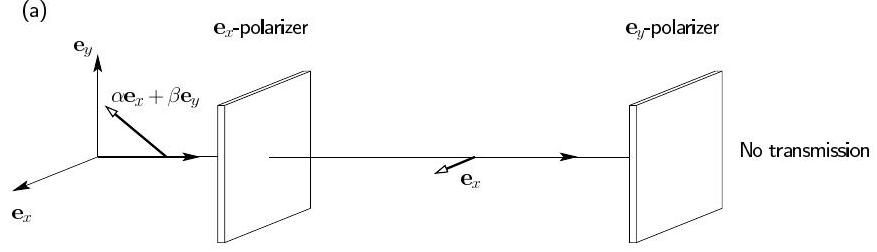
\includegraphics[width=12cm]{2023_12_20_5d48e1c38160b1e32b28g-03}
\end{center}

(b) $\quad \frac{1}{\sqrt{2}}\left(\mathbf{e}_{x}+\mathbf{e}_{y}\right)$-polarizer

\begin{center}
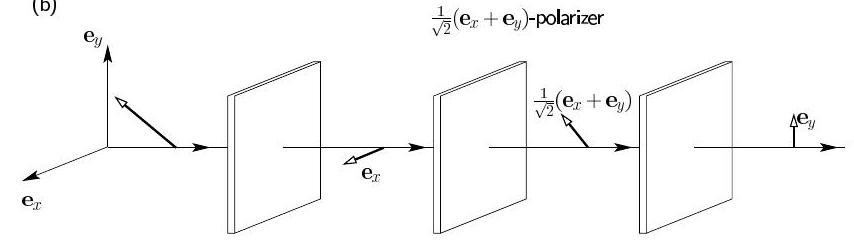
\includegraphics[width=12cm]{2023_12_20_5d48e1c38160b1e32b28g-03(1)}
\end{center}

Figure 14.1 Photon polarization experiment

A-polarized photon. It is a complex number having no obvious physical interpretation of itself, but its magnitude square $|\alpha|^{2}$ is the probability of transmission by an $\mathbf{e}_{x}$-polarizer. Similarly $\beta=\left\langle\mathbf{e}_{y} \mid \mathbf{A}\right\rangle$ is the amplitude for $\mathbf{e}_{y}$-transmission, and $|\beta|^{2}$ the probability of transmission by an $\mathbf{e}_{y}$-polarizer. What is the polarization $A^{\perp}$ such that a polarizer of this type allows for no transmission, $\left\langle\mathbf{A}^{\perp} \mid \mathbf{A}\right\rangle=0$ ? For linearly polarized waves with $\alpha$ and $\beta$ both real we expect it to be geometrically orthogonal, $\mathbf{A}^{\perp}=\beta \mathbf{e}_{x}-\alpha \mathbf{e}_{y}$. For circularly polarized waves, the orthogonal 'direction' is the opposite circular sense. Hence

$$
\frac{1}{\sqrt{2}}\left(\mathbf{e}_{x} \pm i \mathbf{e}_{y}\right)^{\perp}=\frac{1}{\sqrt{2}}\left(\mathbf{e}_{x} \mp i \mathbf{e}_{y}\right) \equiv \mp \frac{1}{\sqrt{2}}\left(i \mathbf{e}_{x}-\mathbf{e}_{y}\right)
$$

since phase factors such as $\pm i$ are irrelevant. In the general elliptical case we might guess that $\mathbf{A}^{\perp}=\bar{\beta} \mathbf{e}_{x}-\bar{\alpha} \mathbf{e}_{y}$, since it reduces to the correct answer for linear and circular polarization. Solving for $\mathbf{e}_{x}$ and $\mathbf{e}_{y}$ we have

$$
\mathbf{e}_{x}=\bar{\alpha} \mathbf{A}+\beta \mathbf{A}^{\perp}, \quad \mathbf{e}_{y}=\bar{\beta} \mathbf{A}-\alpha \mathbf{A}^{\perp}
$$

Let $\mathbf{B}=\gamma \mathbf{e}_{x}+\delta \mathbf{e}_{y}$ be any other polarization, then substituting for $\mathbf{e}_{x}$ and $\mathbf{e}_{y}$ gives

$$
\mathbf{B}=(\gamma \bar{\alpha}+\delta \bar{\beta}) \mathbf{A}+(\gamma \beta-\alpha \delta) \mathbf{A}^{\perp}
$$

Setting $\mathbf{B}=\mathbf{A}$ gives the normalization condition $|\alpha|^{2}+|\beta|^{2}=1$. Hence, since $\langle\mathbf{A} \mid \mathbf{A}\rangle=1$ (transmission probability of 1),

$$
\langle\mathbf{B} \mid \mathbf{A}\rangle=(\gamma \bar{\alpha}+\delta \bar{\beta})=\overline{\langle\mathbf{A} \mid \mathbf{B}\rangle}
$$

Other systems such as the Stern-Gerlach experiment, in which an electron of magnetic moment $\boldsymbol{\mu}$ is always deflected in a magnetic field $\mathbf{H}$ in just two directions, exhibit a completely analogous formalism. The conclusion is that the quantum mechanical states of a system form a complex vector space with inner product $\langle\phi \mid \psi\rangle$ satisfying the usual conditions

$$
\left\langle\phi \mid \alpha \psi_{1}+\beta \psi_{2}\right\rangle=\alpha\left\langle\phi \mid \psi_{1}\right\rangle+\beta\left\langle\phi \mid \psi_{2}\right\rangle \quad \text { and } \quad\langle\phi \mid \psi\rangle=\overline{\langle\psi \mid \phi\rangle} \text {. }
$$

The probability of obtaining a value corresponding to $\phi$ in a measurement is

$$
P(\phi, \psi)=|\langle\phi \mid \psi\rangle|^{2}
$$

As will be seen, states are in fact normalized to $\langle\psi \mid \psi\rangle=1$, so that only linear combinations $\alpha \psi_{1}+\beta \psi_{2}$ with $|\alpha|^{2}+|\beta|^{2}=1$ are permitted.

\subsection{态的希尔伯特空间}(填充)
\subsection{可观测量}(填充)
\subsection{量子力学中的无界算符}(填充)
\section{量子动力学}(填充)
\subsection{海森堡图景}(填充)
\subsection{经典力学和波动力学的对应关系}(填充)
\subsection{谐振子}(填充)
\subsection{角动量}(填充)
\section{对称变换}(填充)
\subsection{无穷小生成元}(填充)
\subsection{粒子数守恒}(填充)
\subsection{离散对称性}(填充)
\subsection{全同粒子}(填充)
\section{量子统计力学}(填充)
\subsection{密度算符}(填充)
\subsection{系综}(填充)
\subsection{全同粒子体系}(填充)
\chapter{微分几何}(填充)
\section{可微流形}(填充)
\section{可微映射和曲线}(填充)
\section{切空间,余切空间和张量空间}(填充)
\subsection{切矢量}(填充)
\subsection{余切空间和张量空间}(填充)
\subsection{向量和张量场}(填充)
\subsection{坐标变换}(填充)
\subsection{张量丛}(填充)
\section{切映射和子流形}(填充)
\subsection{切映射和映射的拉回}(填充)
\subsection{子流形}(填充)
\section{对易子,流和李导数}(填充)
\subsection{对易子}(填充)
\subsection{积分曲线和流}(填充)
\section{分布和Frobenius定理}(填充)
\chapter{可微形式}(填充)
\section{微分形式和外导数}(填充)
\section{外导数的性质}(填充)
\section{Frobenius定理:对偶形式}(填充)
\section{热力学}(填充)
\subsection{热力学第二定律}(填充)
\subsection{绝对熵和温度}(填充)
\section{经典力学}(填充)
\subsection{变分学}(填充)
\subsection{拉格朗日力学}(填充)
\subsection{哈密顿力学}(填充)
\subsection{拉格朗日力学和哈密顿力学之间的联系}(填充)
\chapter{流形上的积分}(填充)
\section{单位分解}(填充)
\section{n-形式的积分}(填充)
\section{stokes定理}(填充)
\subsection{常规定义域}(填充)
\section{同调和上同调}(填充)
\subsection{有序单纯形和欧氏空间中的链}(填充)
\subsection{流形上的单纯同调}(填充)
\subsection{De Rham上同调群和对偶性}(填充)
\section{庞加莱引理}(填充)
\subsection{电动力学}(填充)
\chapter{联络和曲率}(填充)
\section{线性联络和测地线}(填充)
\subsection{坐标变换}(填充)
\section{张量场的协变导数}(填充)
\section{曲率和挠率}(填充)
\subsection{挠率张量}(填充)
\subsection{曲率张量}(填充)
\section{伪黎曼流形}(填充)
\subsection{黎曼联络}(填充)
\subsection{测地坐标}(填充)
\section{测地偏离方程}(填充)
\section{黎曼张量及其对称性}(填充)
\subsection{比安基恒等式}(填充)
\section{嘉当标准形}(填充)
\subsection{嘉当标准形中的伪黎曼空间}(填充)
\subsection{局域平直空间}(填充)
\section{广义相对论}(填充)
\subsection{等效原理}(填充)
\subsection{广义相对论的基本假设}(填充)
\subsection{曲率张量的测量}(填充)
\subsection{线性近似}(填充)
\subsection{史瓦西解}(填充)
\section{宇宙学}(填充)
\section{时空的变分原理}(填充)
\subsection{希尔伯特作用量}(填充)
\subsection{场的能动张量}(填充)
\chapter{李群和李代数}(填充)
\section{李群}(填充)
\subsection{左不变向量场}(填充)
\subsection{李群的李代数}(填充)
\subsection{Maurer-Cartan关系}(填充)
\section{指数映射}(填充)
\subsection{指数映射}(填充)
\section{李子群}(填充)
\subsection{矩阵李群}(填充)
\section{李群的变换}(填充)
\subsection{正规子群}(填充)
\section{保度规群}(填充)
\subsection{球对称}(填充)


\end{document}